% figures/latex_includes.tex
% 由 _tmp/gen_latex_includes.py 生成：题注中每个数字均在生成时从
% figures/*.json 现读，未从报告或正文手抄。请勿手工编辑本文件。
% 图序与 PROBLEM_ANALYSIS.md 的 FIGURE_MANIFEST 数据图段落一致，共 32 张。

\begin{figure}[H]
  \centering
  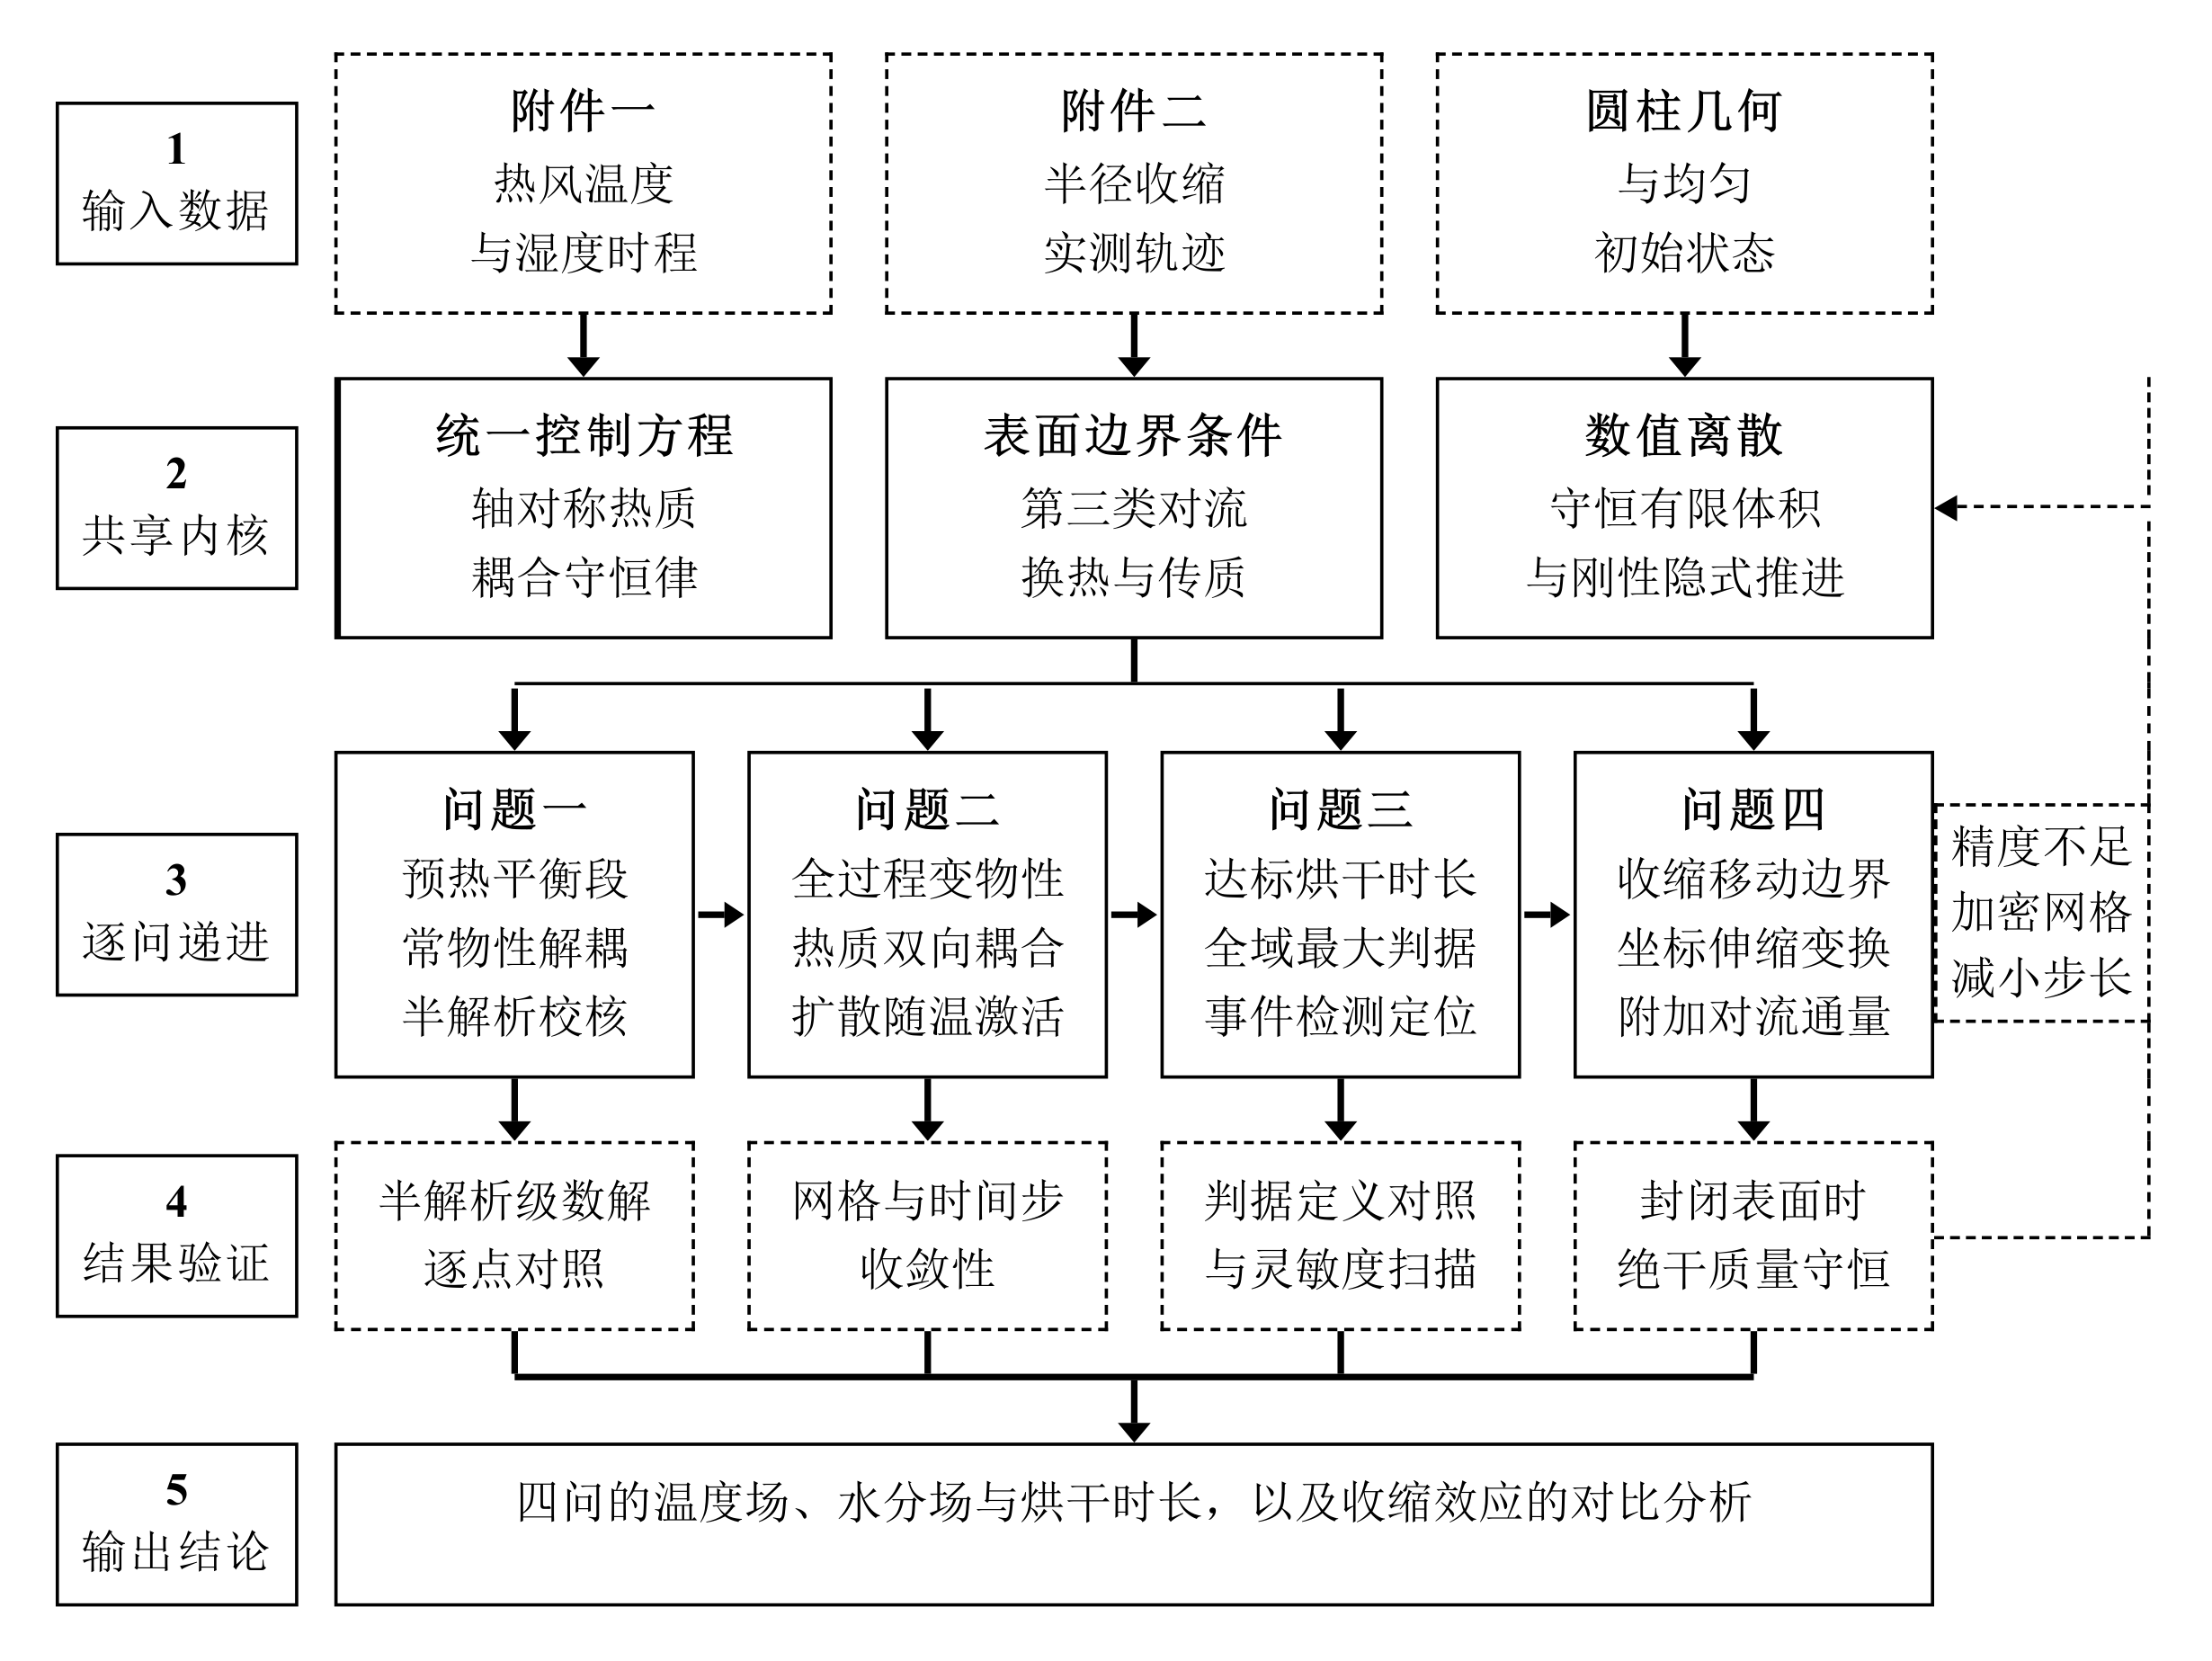
\includegraphics[width=0.98\textwidth]{figures/fig_roadmap.png}
  \caption[全文建模与求解路线]{全文建模与求解路线。自附件 1 的热风工况与附件 2 的半径轨迹出发，经"轴对称热质耦合控制方程—径向有限体积离散—四级模型阶梯校核"三层，分支到四个问题：问题一预热段温度场、问题二三小时热质耦合场、问题三达标烘干时长与敏感度、问题四收缩几何下的复算与对照。虚线回路表示由校核结果回到离散与参数标定的迭代；各问共用同一套物性与同一份网格判据，故结果可横向比较。}
  \label{fig:roadmap}
\end{figure}

\begin{figure}[H]
  \centering
  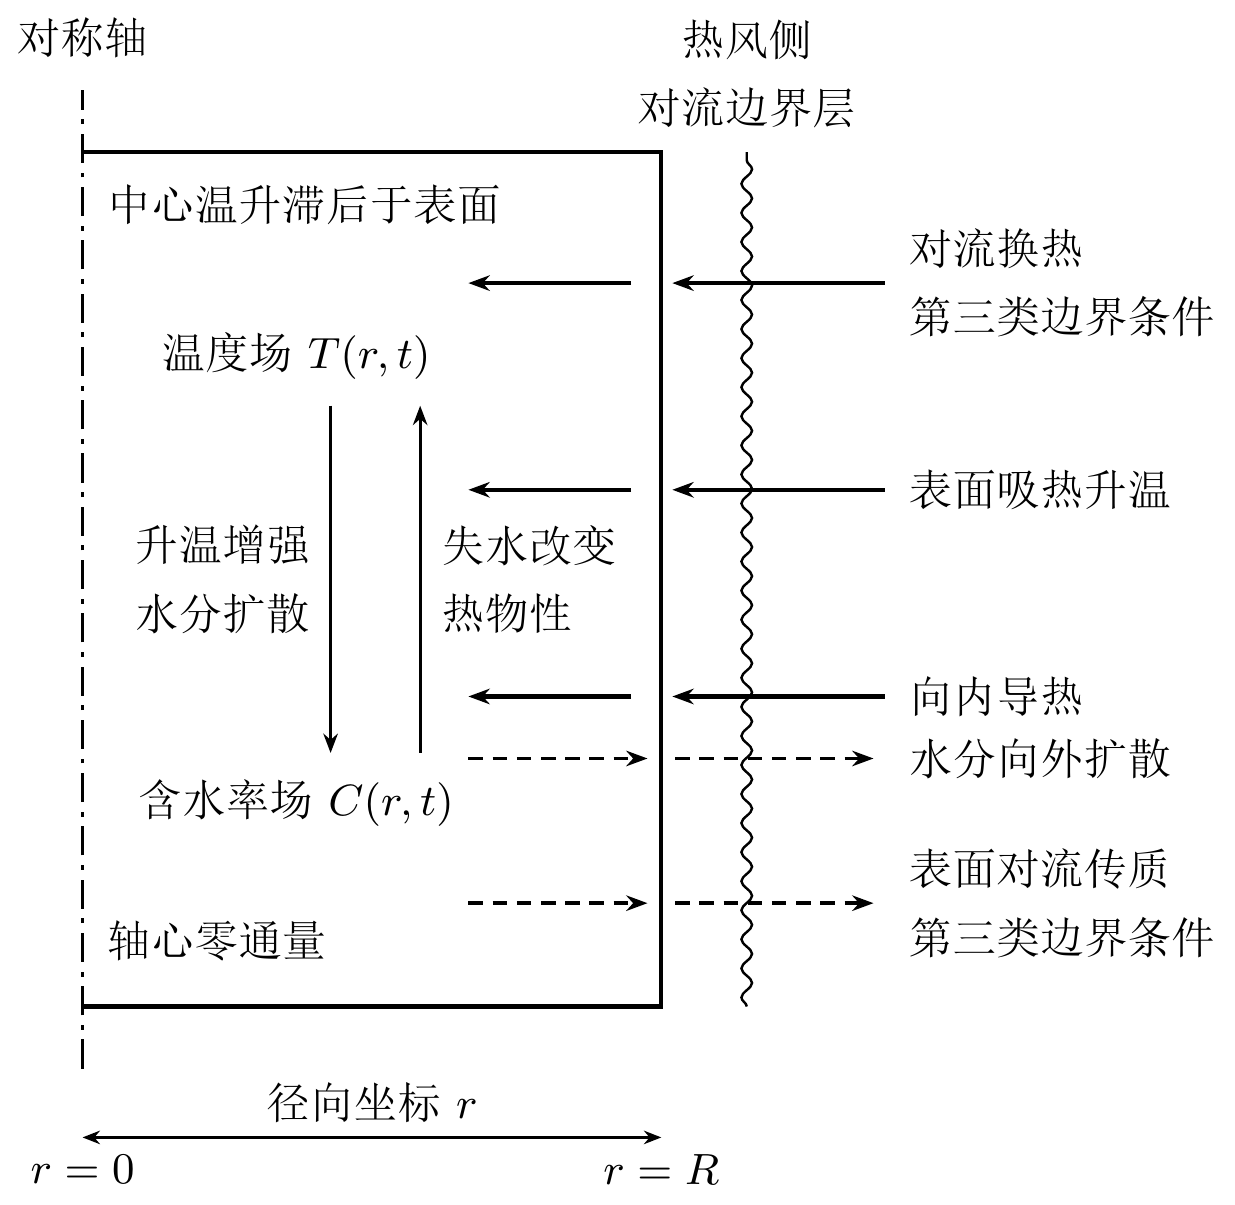
\includegraphics[width=0.72\textwidth]{figures/tikz_mechanism_heatmass.png}
  \caption[热质耦合传递机理]{热质耦合传递机理示意。药材按无限长圆柱处理，只保留径向，左缘为对称轴、右缘为受热与传质表面。表面同时承受对流换热（第三类边界条件）与对流传质，两者通过两条竖直箭头表示的双向耦合联系：升温增强水分扩散，蒸发吸热又抑制升温。轴心处两个场的通量均为零，该条件在守恒离散下自动满足而无需另行施加。}
  \label{fig:tikz_mechanism_heatmass}
\end{figure}

\begin{figure}[H]
  \centering
  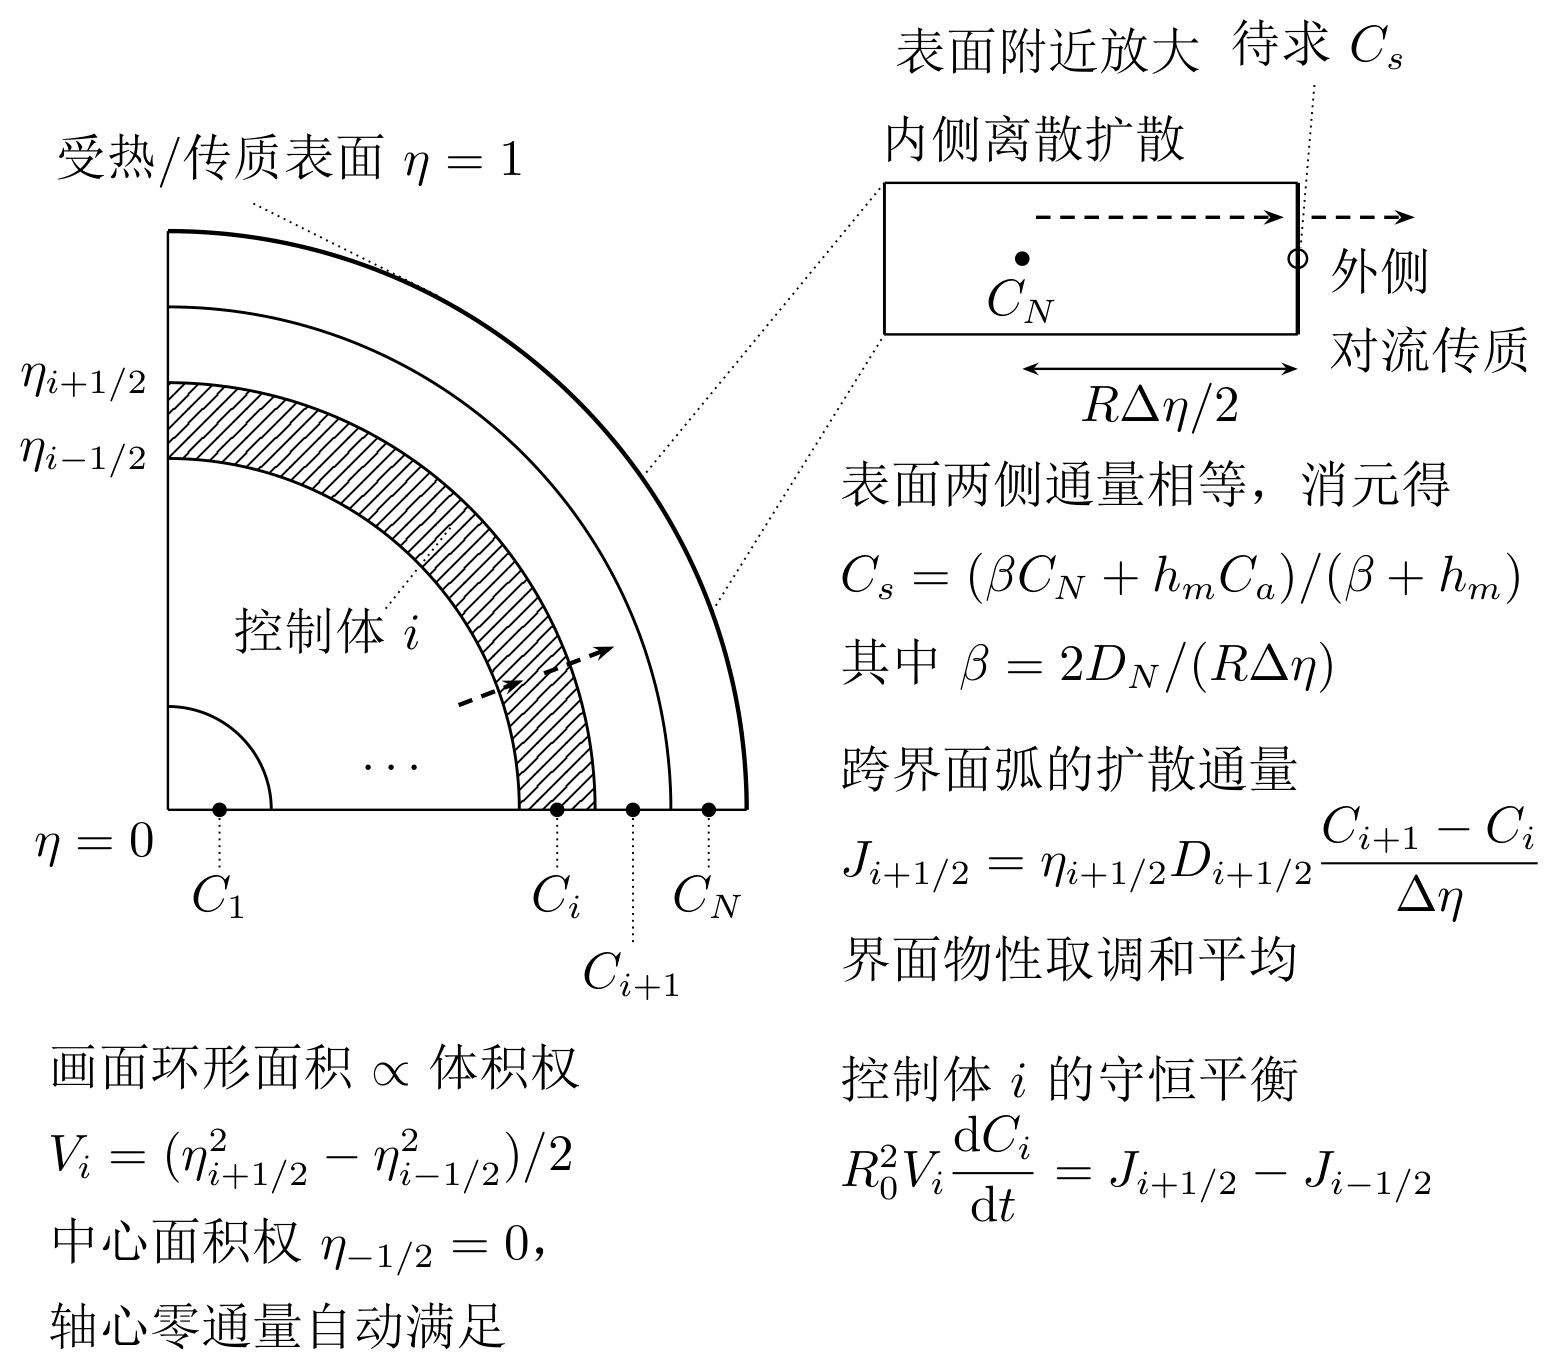
\includegraphics[width=1.00\textwidth]{figures/tikz_derive_fvm.png}
  \caption[径向有限体积离散与表面值反解]{径向有限体积离散与表面值反解。左侧四分之一截面示意环形控制体的划分：图上环形面积即体积权 $V_i=(\eta_{i+1/2}^{2}-\eta_{i-1/2}^{2})/2$，中心控制体的面积权退化为零，故轴心零通量自动成立。跨界面弧的扩散通量按界面物性的调和平均取值，控制体的变化率仅由两个界面通量之差给出，逐格求和后总量守恒。右上放大图给出本题的关键：格心不落在表面上，相距半个网格 $R\Delta\eta/2$；内侧离散扩散与外侧对流传质写的是同一个表面通量，消元即得表面值 $C_s$，无须把边界条件降阶为一阶差分。}
  \label{fig:tikz_derive_fvm}
\end{figure}

\begin{figure}[H]
  \centering
  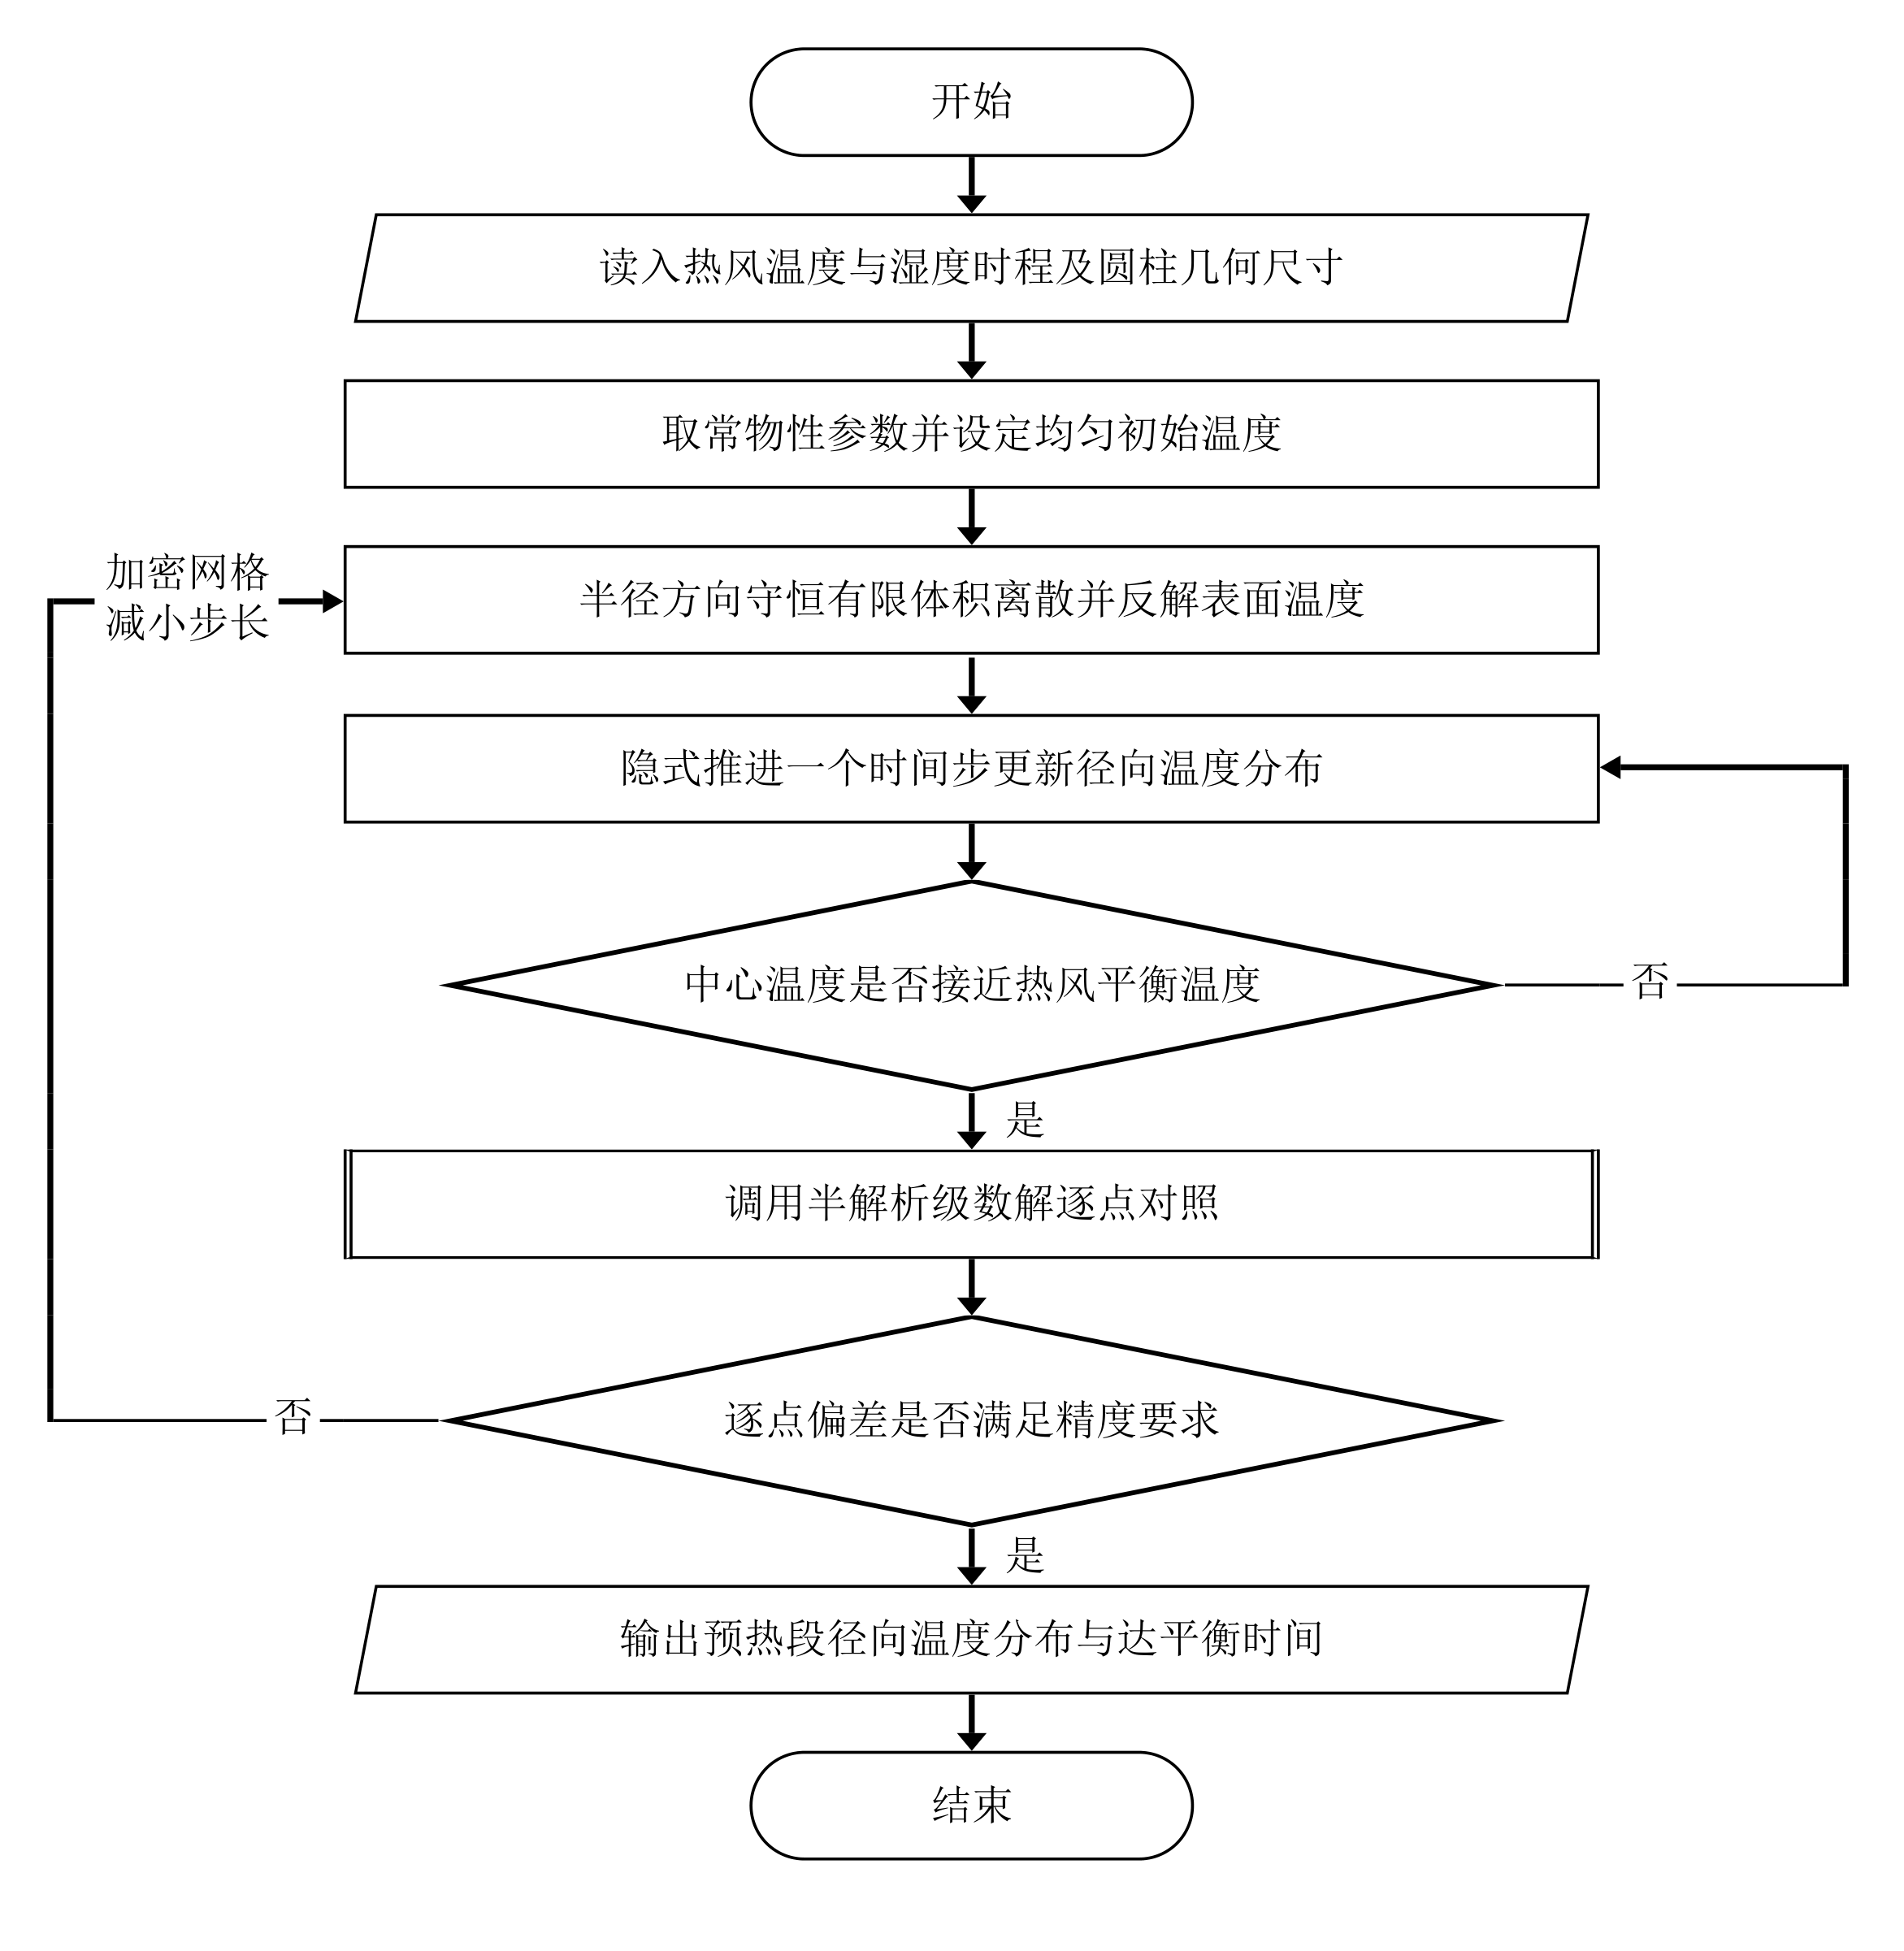
\includegraphics[width=0.95\textwidth]{figures/fig_flow_q1.png}
  \caption[问题一求解流程]{问题一求解流程。输入为附件 1 前 1800\,s 的 31 个热风实测点，经插值驱动、纯导热方程的径向有限体积离散、隐式时间推进，输出温度场并以两条独立判据收口：半解析级数解逐点比对与 5 档网格无关性检验，任一判据不达容差即退回加密网格或缩短时间步。}
  \label{fig:flow_q1}
\end{figure}

\begin{figure}[H]
  \centering
  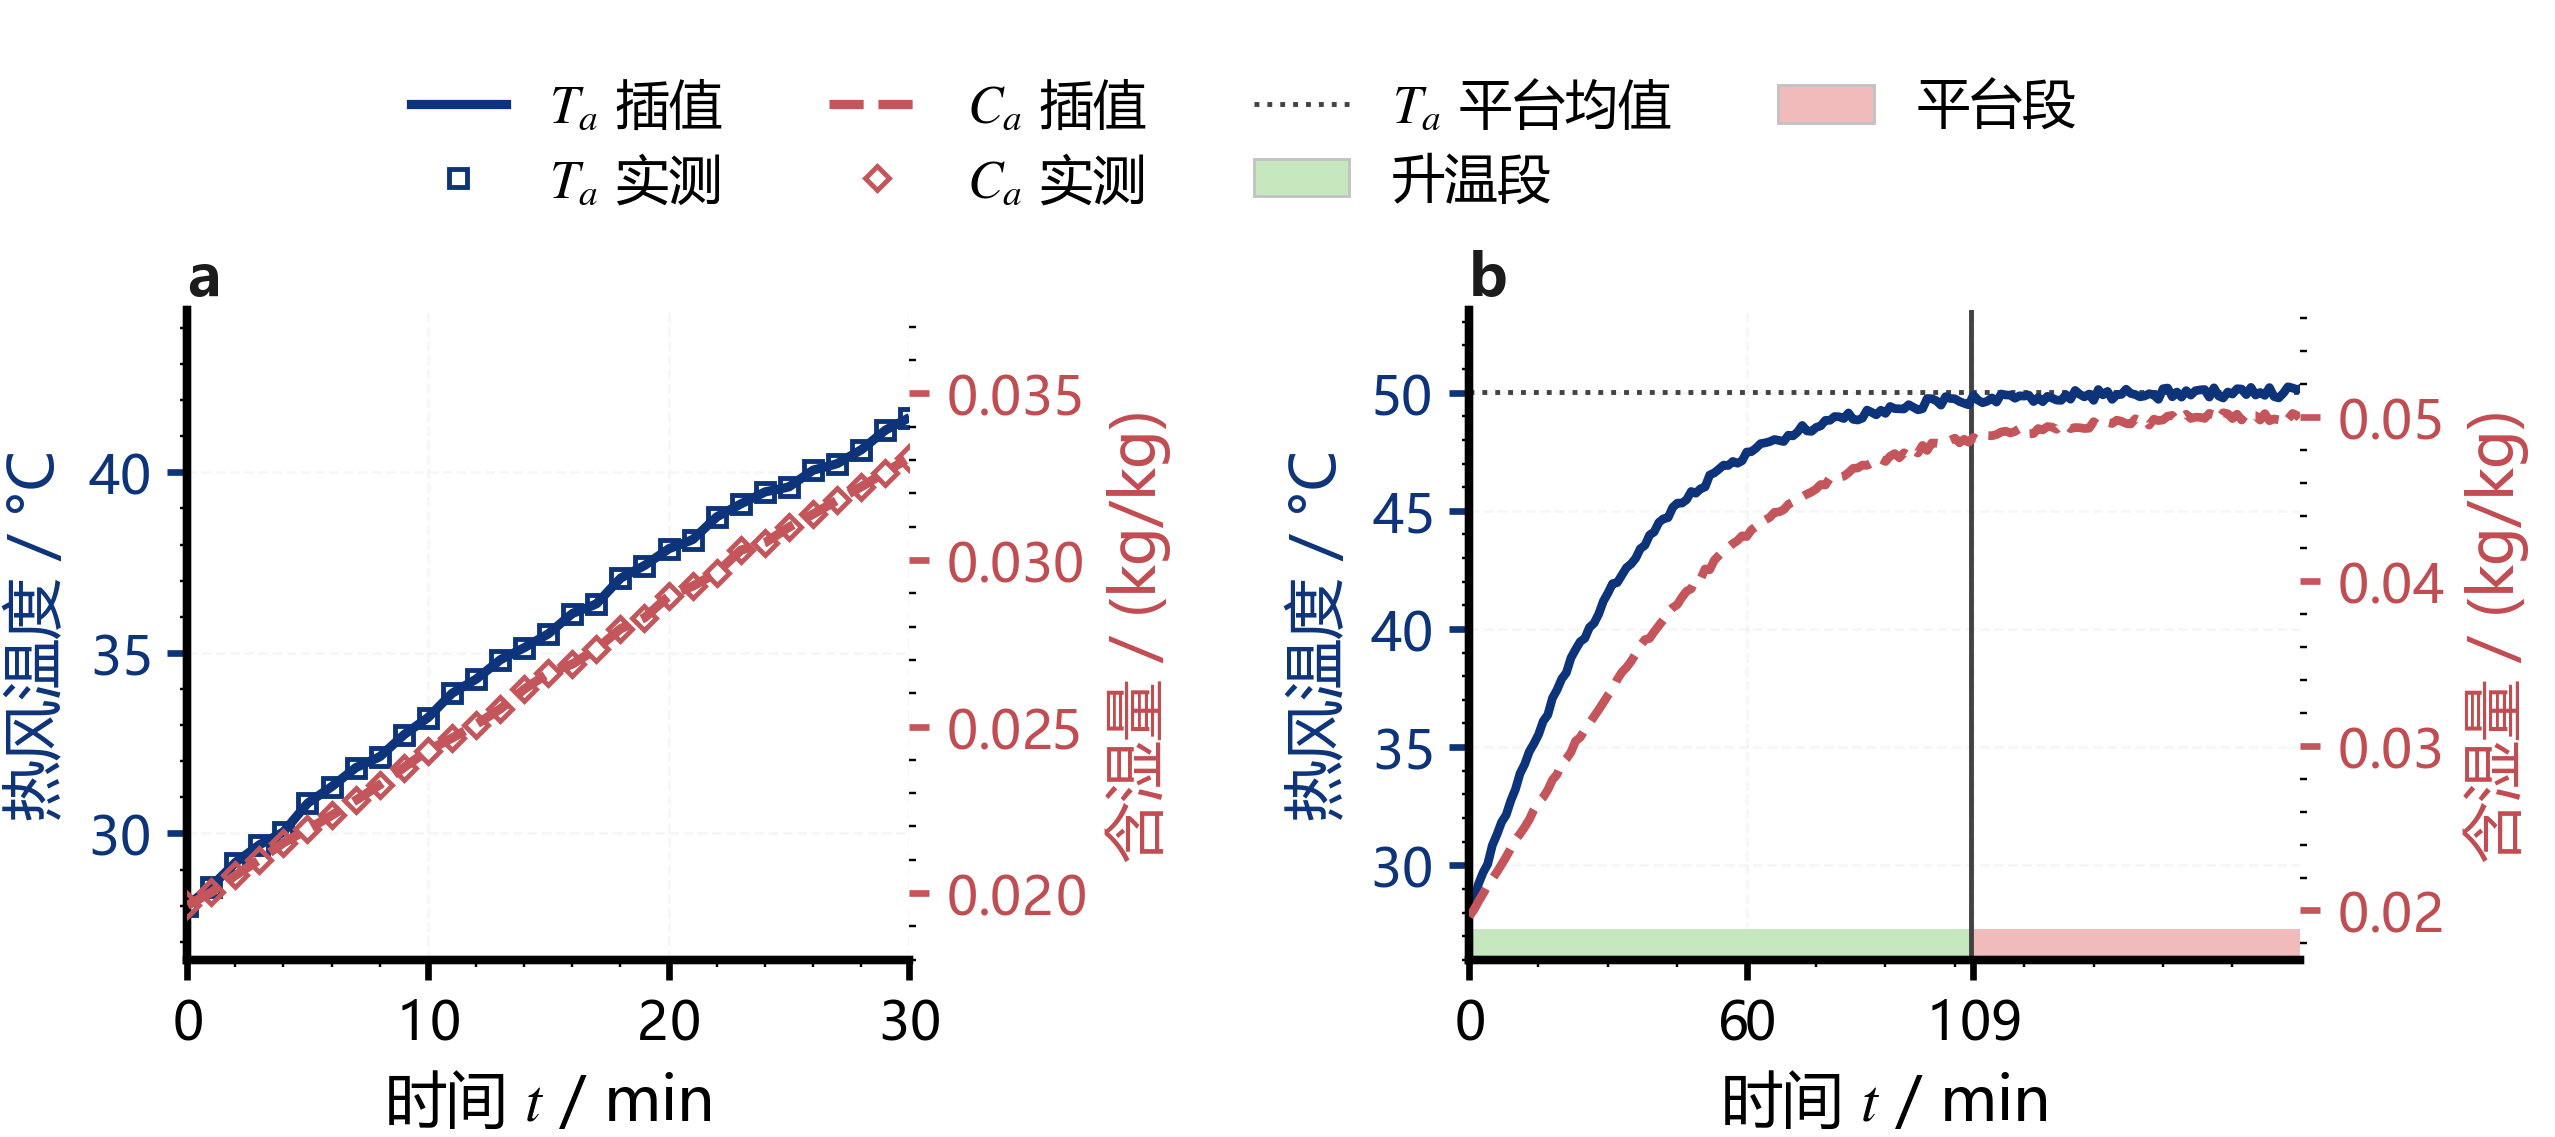
\includegraphics[width=1.00\textwidth]{figures/fig_q1_air_input.png}
  \caption[附件 1 热风温度与空气含湿量时程]{附件 1 热风温度与空气含湿量的双轴时程。面板 a 为问题一预热窗口（0--1800\,s，31 个实测点），热风温度自 28.00\,°C 单调升至 41.513\,°C，含湿量同步由 0.01963 升至 0.03307；面板 b 为问题二全 3\,h 窗口，竖线处（$t$=108.5\,min）温度进入 $\pm0.5$\,°C 邻域不再离开，平台均值 50.017\,°C、含湿量均值 0.05001。曲线为 PDE 实际调用的插值驱动，实测点复现相对误差 0（判据 $<10^{-9}$）。}
  \label{fig:q1_air_input}
\end{figure}

\begin{figure}[H]
  \centering
  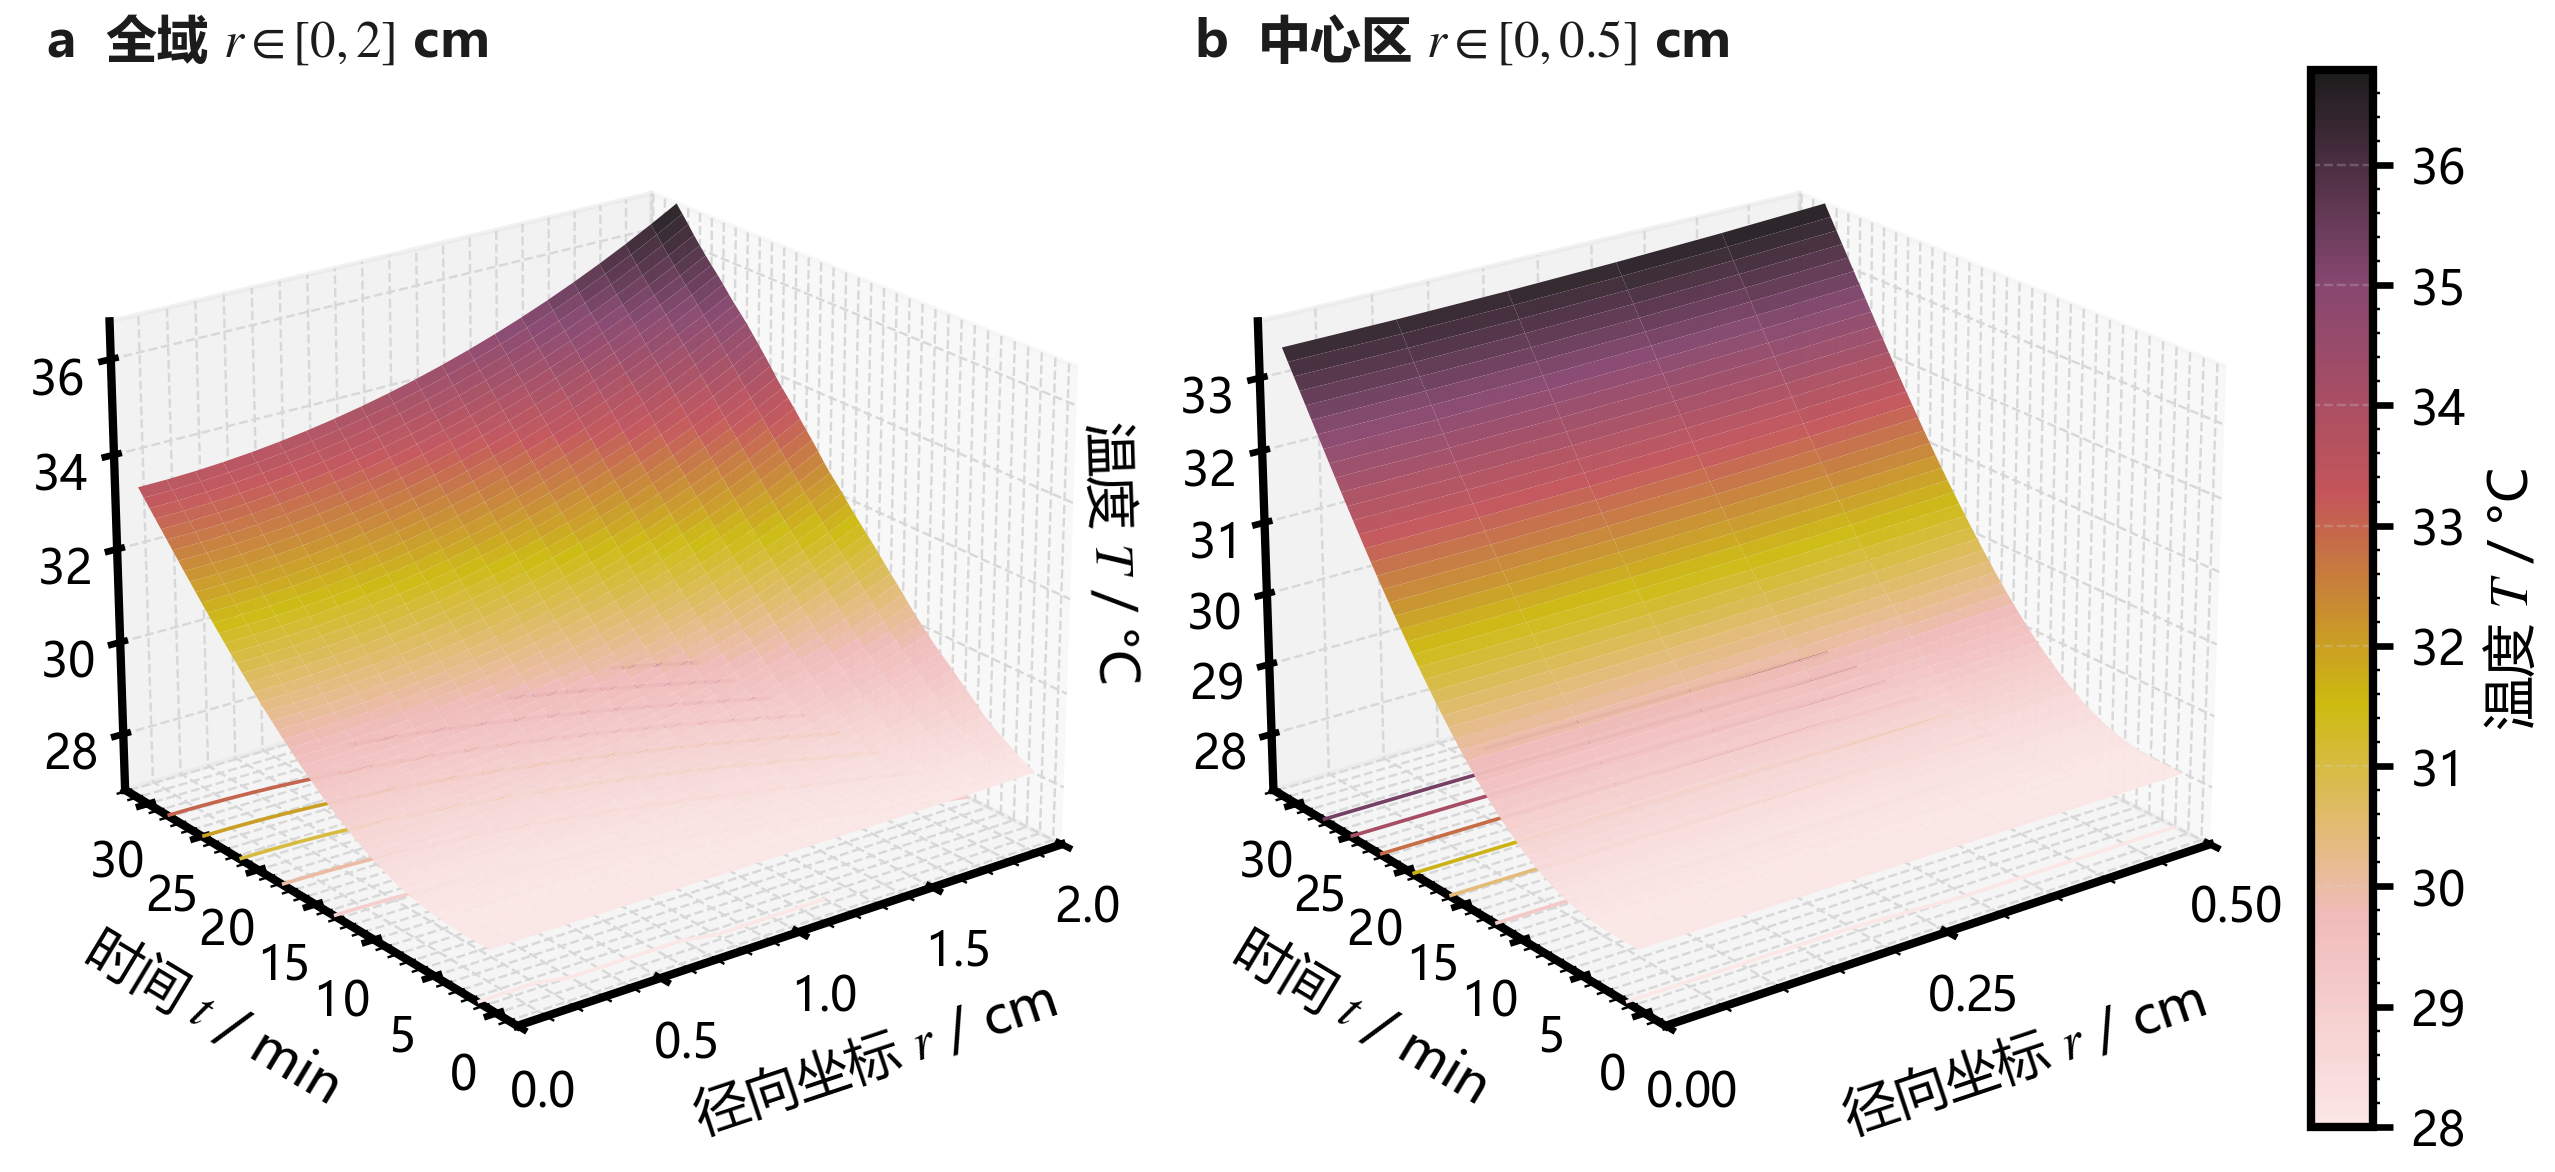
\includegraphics[width=1.00\textwidth]{figures/fig_q1_temp_field_3d.png}
  \caption[问题一预热段温度场三维曲面]{问题一预热段温度场 $T(r,t)$ 的三维曲面与底面等值线投影。面板 a 覆盖全域 $r\in[0,R_0]$，面板 b 放大中心区 $r\in[0,0.5]$\,cm。温度跨度 28.00--36.79\,°C；1800\,s 时表面 36.786\,°C、中心 33.575\,°C，中心—表面温差 3.210\,°C，热渗透深度 $\sqrt{\alpha t}$=0.2981\,cm。}
  \label{fig:q1_temp_field_3d}
\end{figure}

\begin{figure}[H]
  \centering
  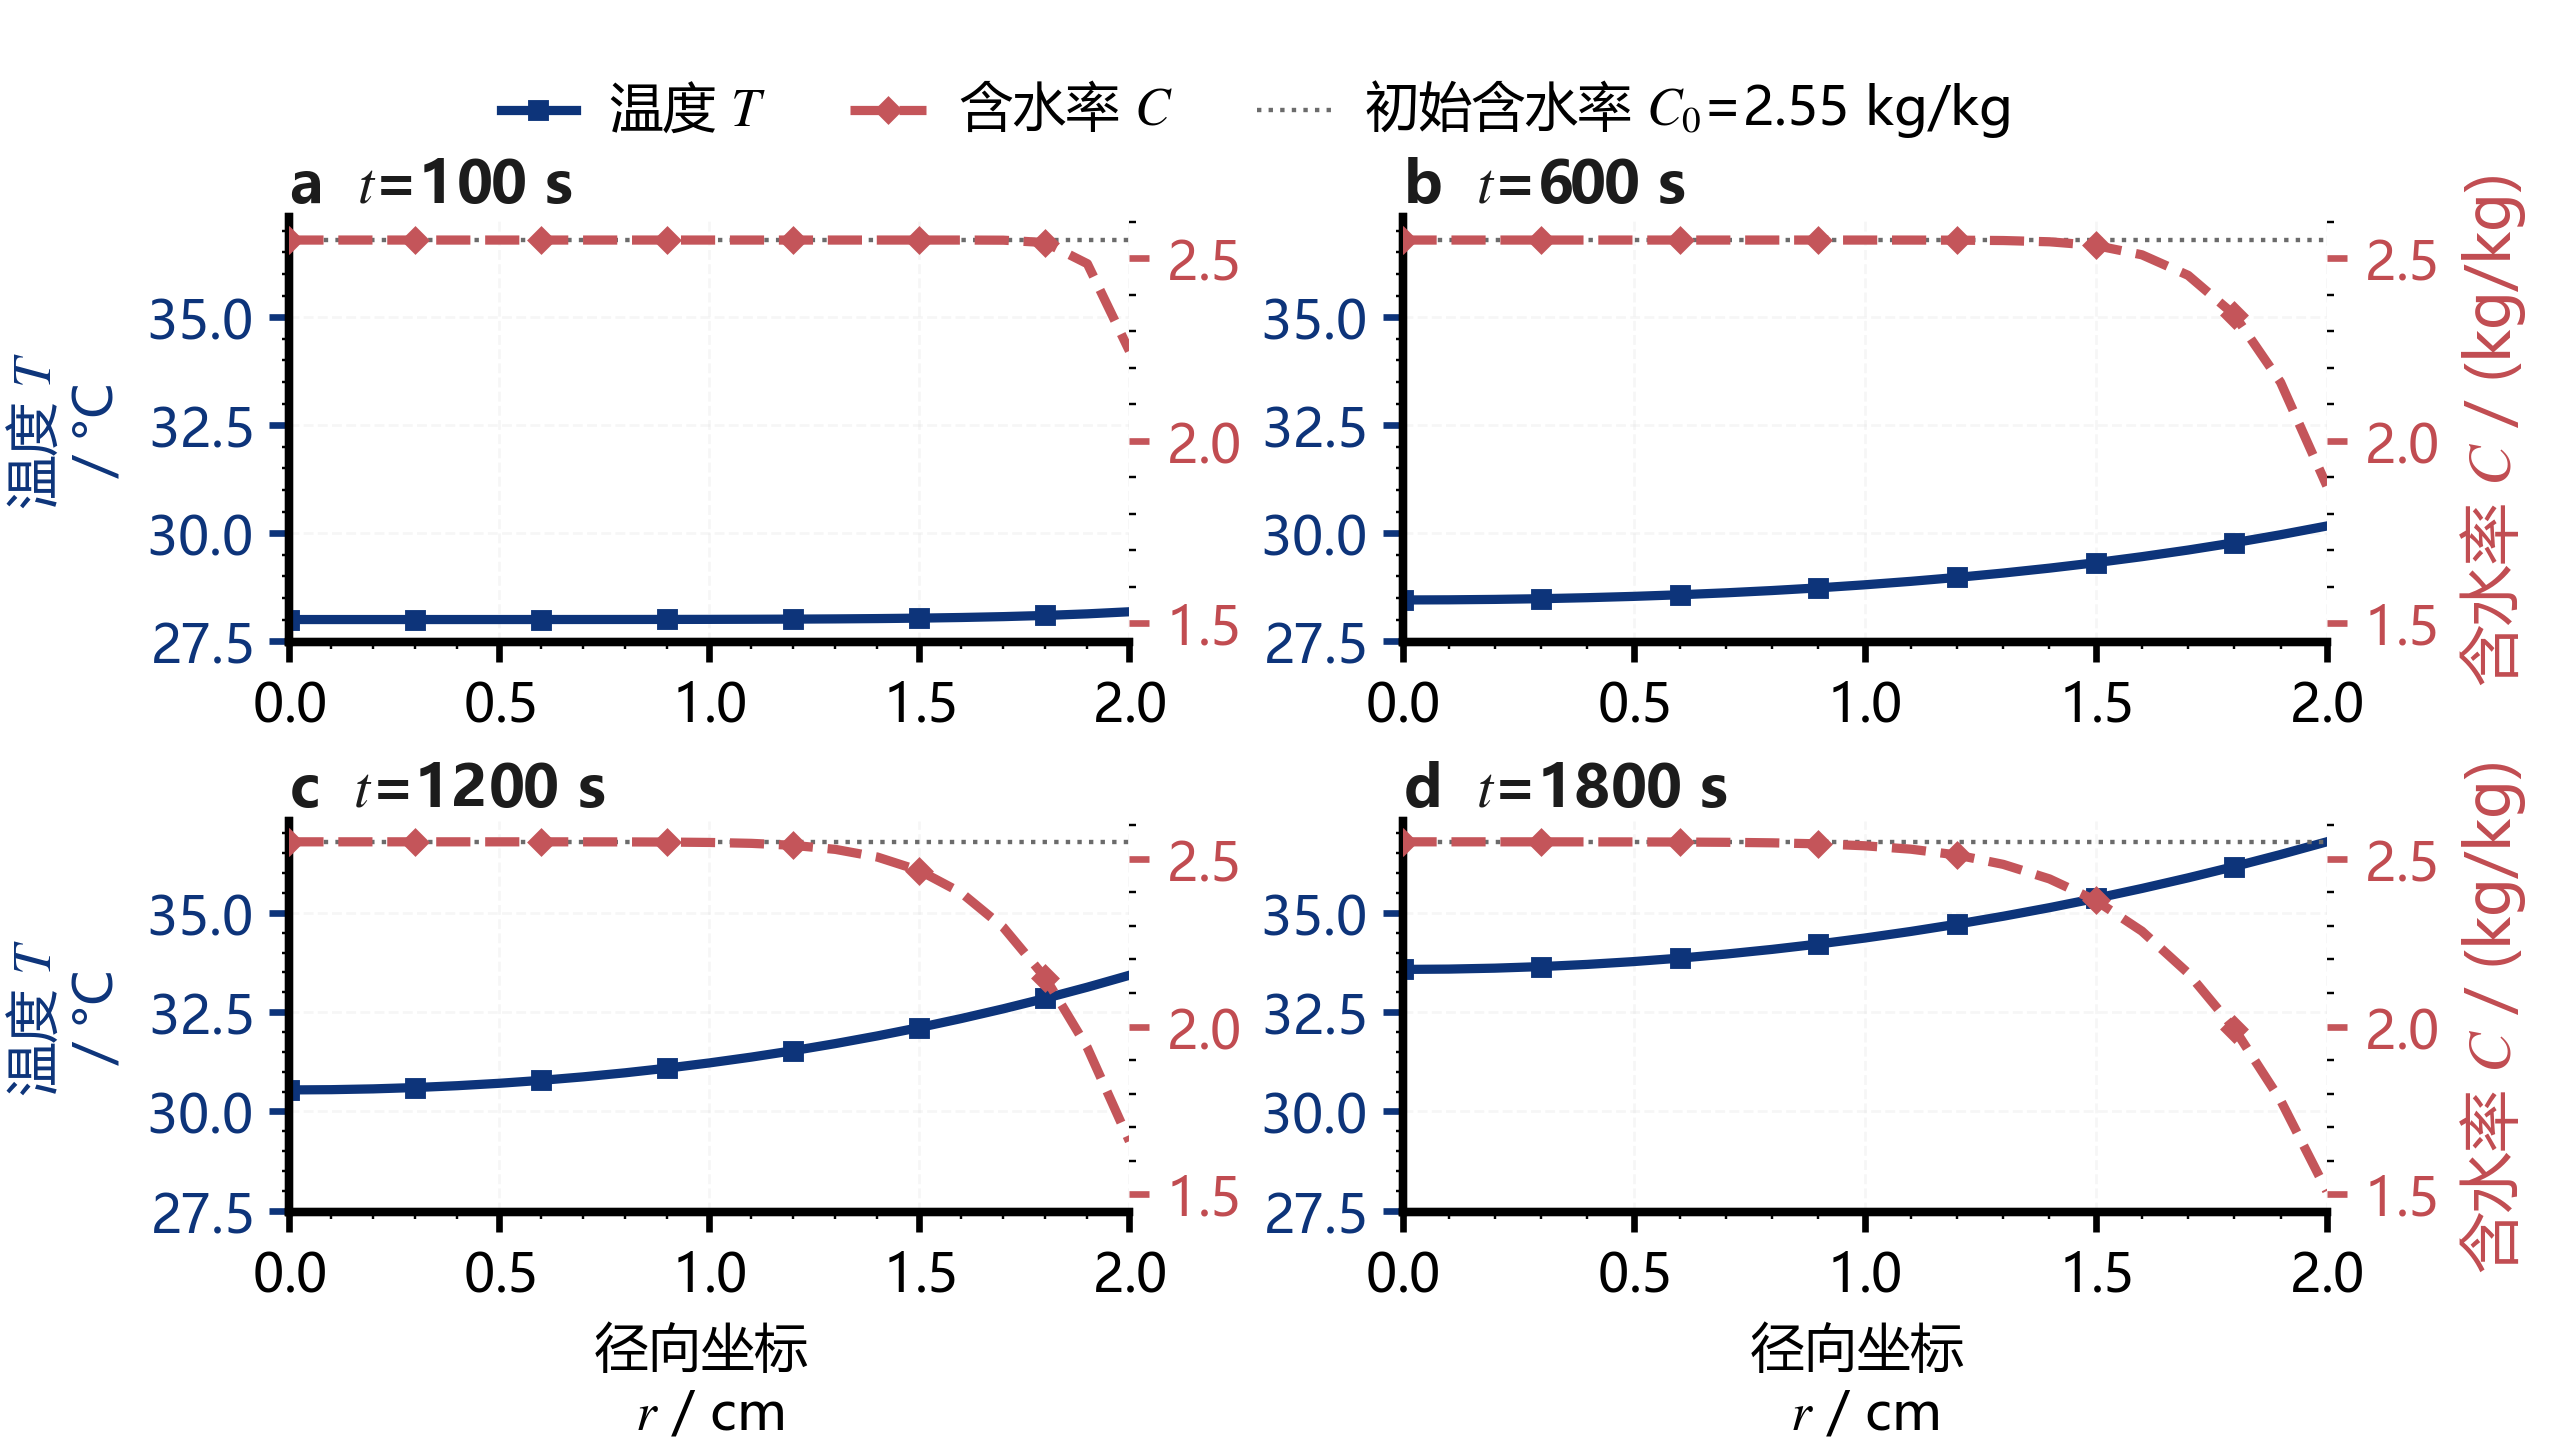
\includegraphics[width=1.00\textwidth]{figures/fig_q1_profiles_frames.png}
  \caption[问题一四时刻径向剖面]{问题一四个时刻（100/600/1200/1800\,s）的径向剖面小多图，温度与含水率同框双轴。含水率在 1800\,s 仍呈边界层形态：表面 1.5102\,kg/kg，中心 2.5500\,kg/kg（相对 $C_0$=2.55 仅降 $7.86\times10^{-6}$），体积平均 2.2936\,kg/kg。热扰动已贯穿全域而质扰动尚未到达中心，对应 $Bi_T$=1.3889 与 $Bi_m$=3.2404 的量级差。}
  \label{fig:q1_profiles_frames}
\end{figure}

\begin{figure}[H]
  \centering
  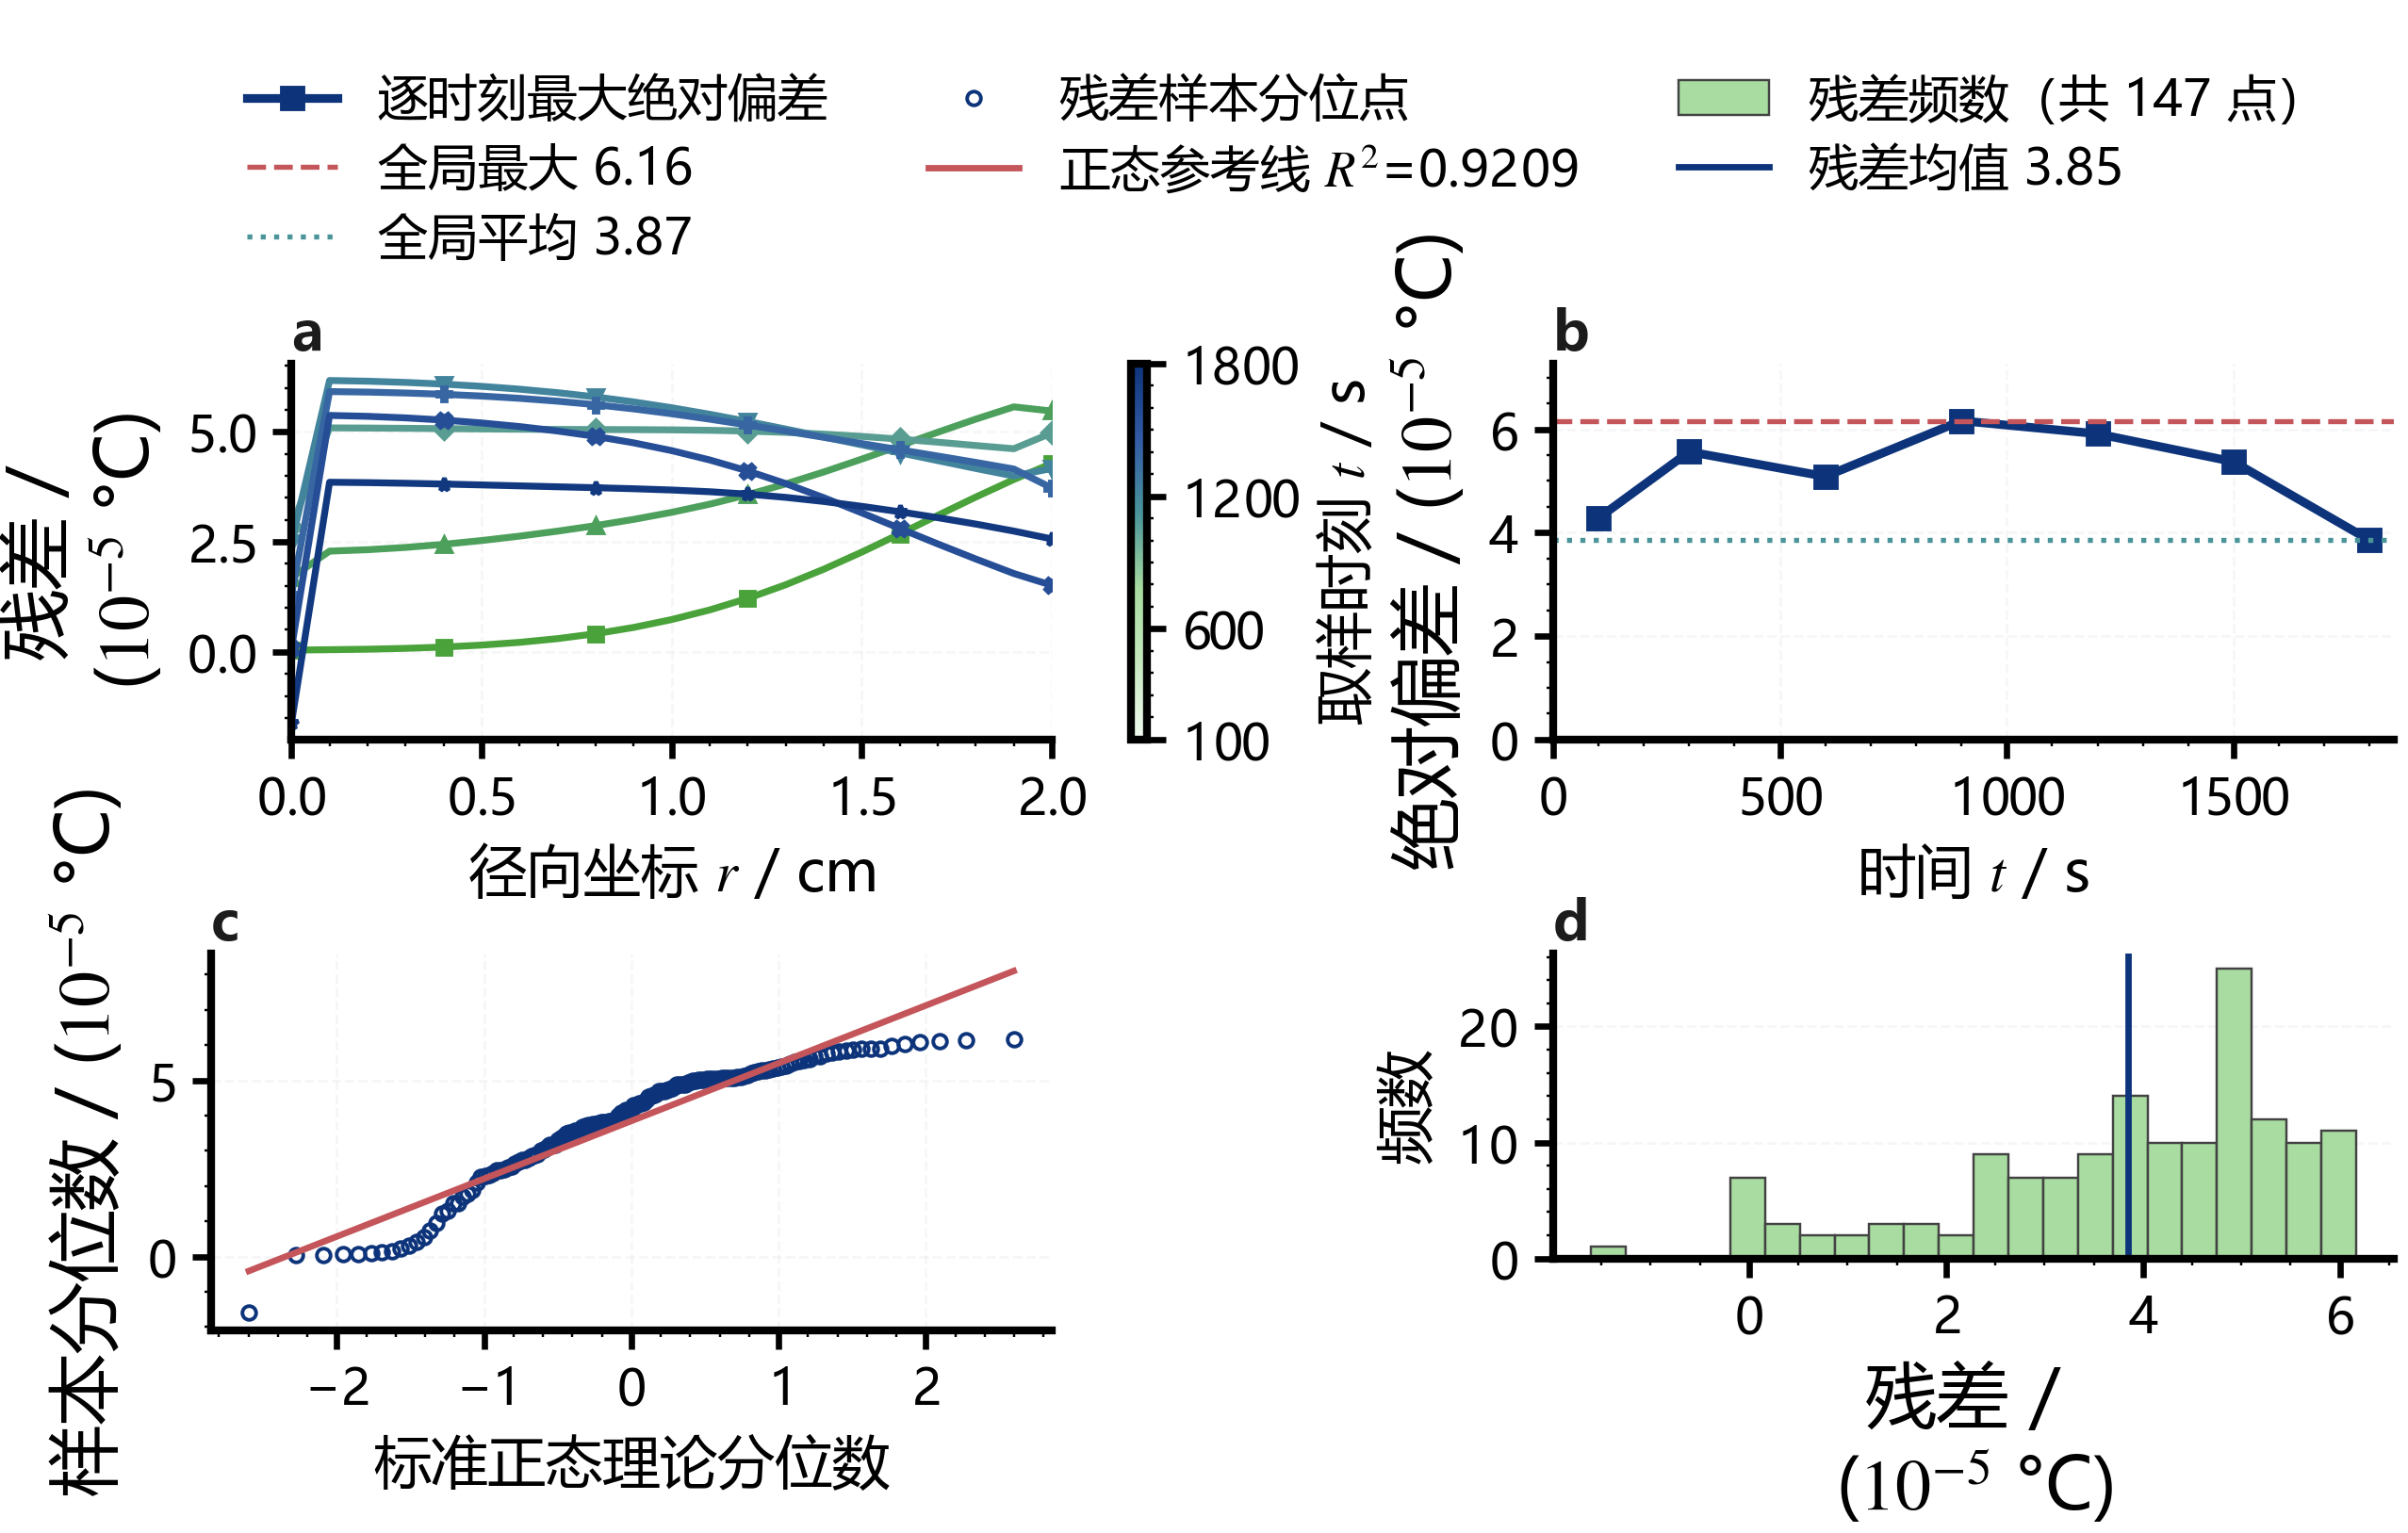
\includegraphics[width=1.00\textwidth]{figures/fig_q1_validate_analytic.png}
  \caption[半解析级数解与有限体积解的残差诊断]{Duhamel--Bessel 半解析级数解与守恒型有限体积解的四联残差诊断。面板 a 为两解的剖面叠合，b 为逐点残差，c 为残差随时间的极值包络，d 为残差直方图。147 个时空点上最大绝对偏差 $6.16\times10^{-5}$\,°C、平均 $3.87\times10^{-5}$\,°C，远低于 $10^{-2}$\,°C 判据；级数取前 6 阶，首三个特征根 $\beta_n$=1.4185/4.1665/7.2085，对应时间常数 1177.3/136.5/45.6\,s。}
  \label{fig:q1_validate_analytic}
\end{figure}

\begin{figure}[H]
  \centering
  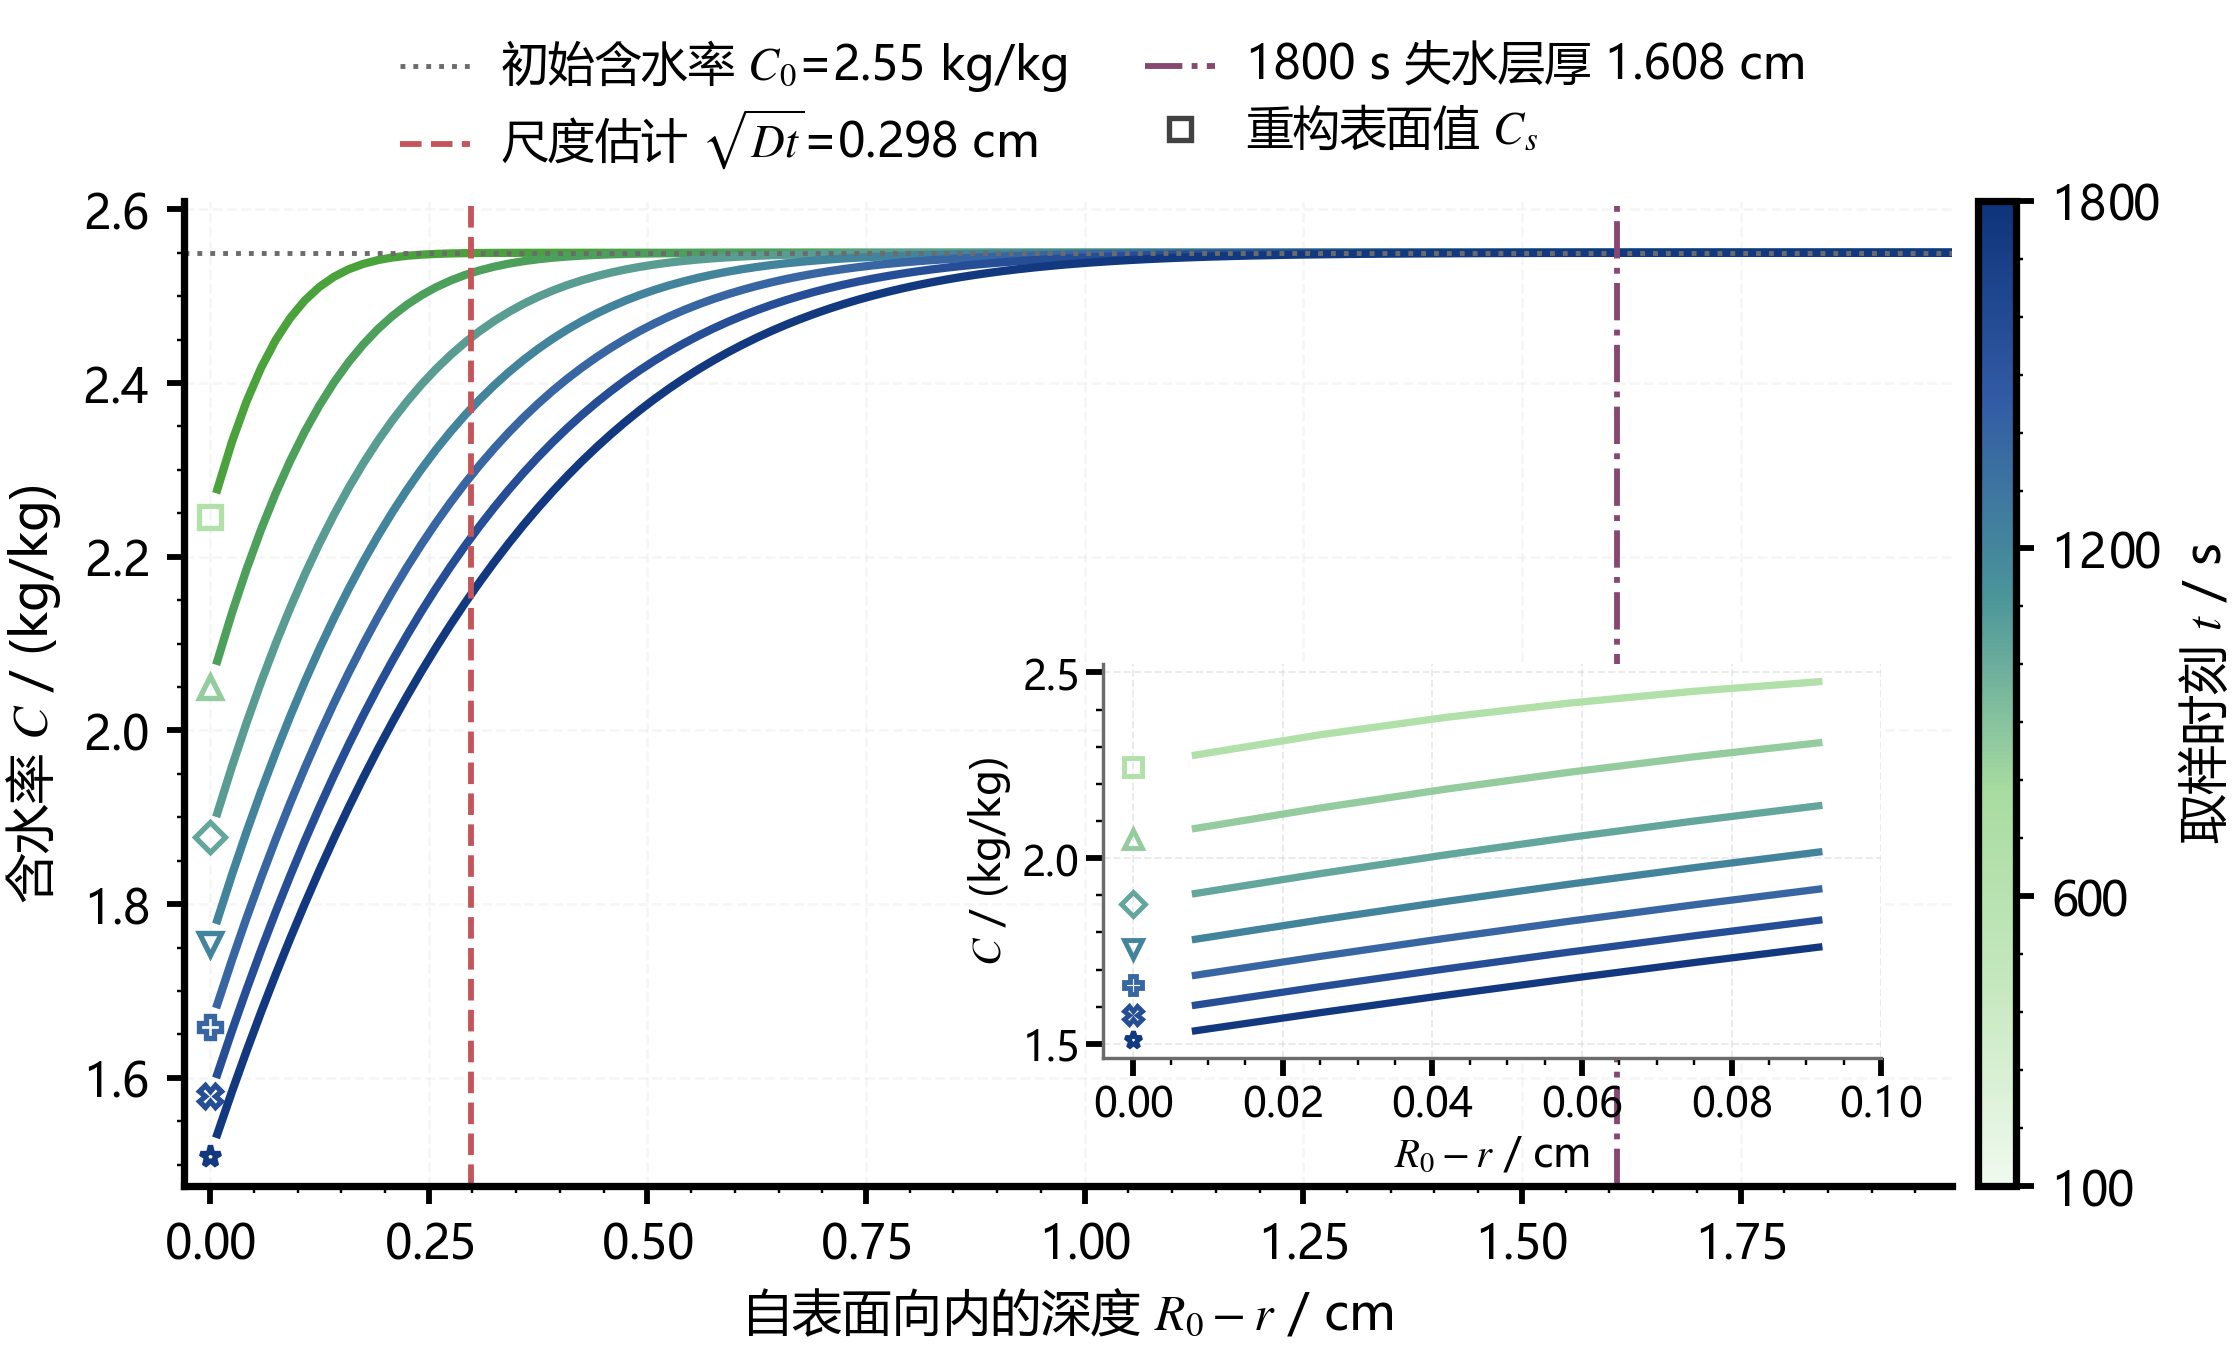
\includegraphics[width=0.92\textwidth]{figures/fig_q1_moisture_bl.png}
  \caption[问题一表面失水边界层]{问题一表面失水边界层：含水率沿自表面度量的深度分布，插图放大近表面 0.1\,cm。以 $C_0-C>10^{-4}$ 为判据，失水层厚度自 100\,s 的 0.3250\,cm 增至 1800\,s 的 1.6083\,cm，与尺度估计 $\sqrt{D t}$=0.2981\,cm 同量级；中心含水率全程保持 2.5500\,kg/kg，故问题一不可用集中参数近似替代 PDE。}
  \label{fig:q1_moisture_bl}
\end{figure}

\begin{figure}[H]
  \centering
  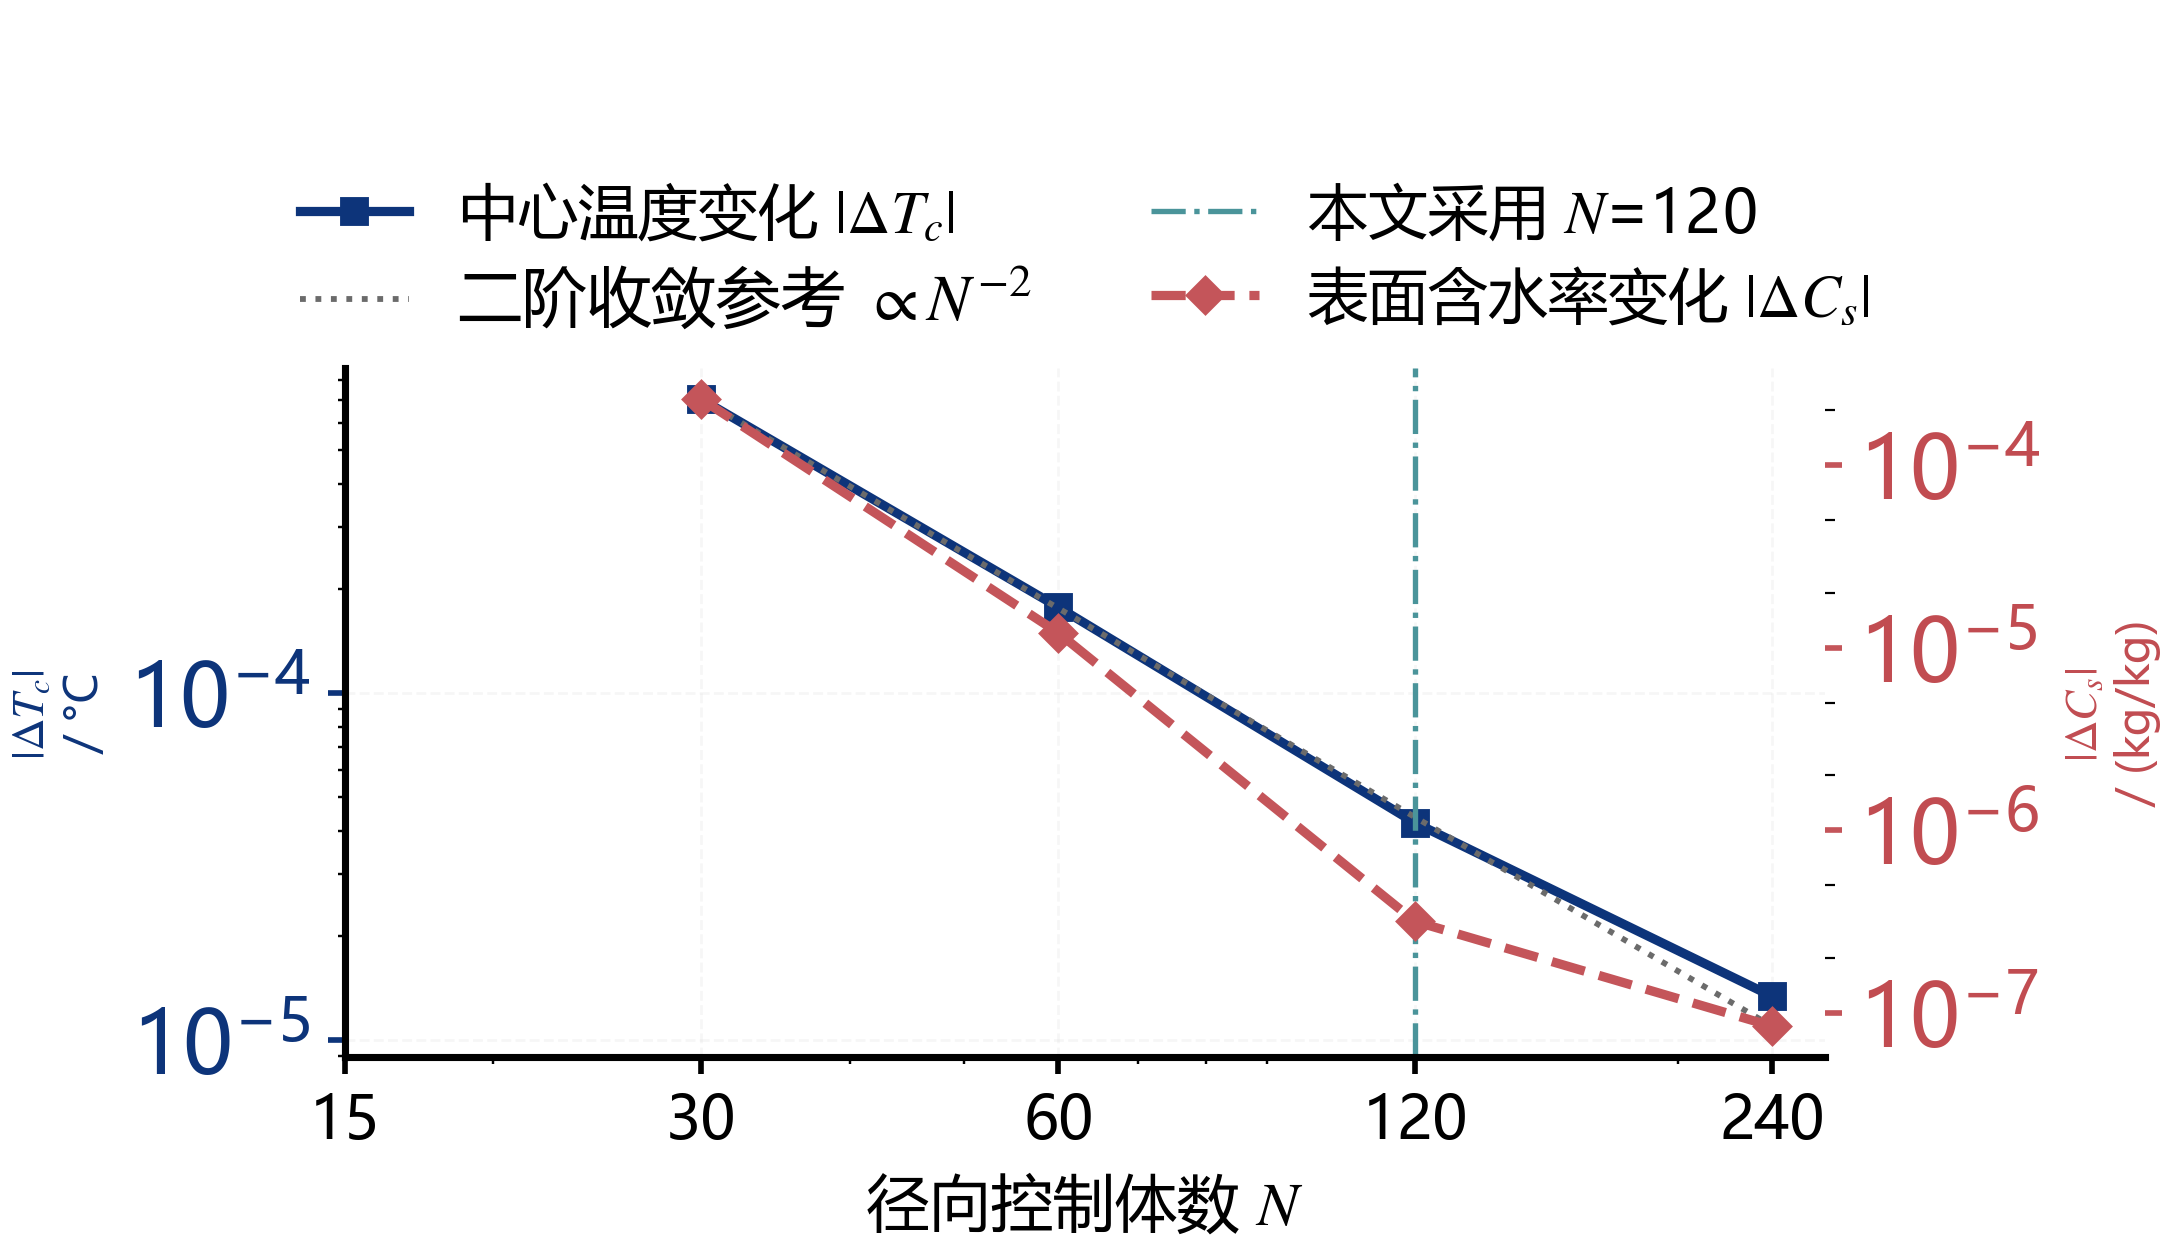
\includegraphics[width=0.86\textwidth]{figures/fig_q1_grid_conv.png}
  \caption[问题一网格无关性验证]{问题一网格无关性：逐次加密的解变化量随控制体数 $N$ 的衰减，灰色参考线为二阶斜率，竖线为本文采用的基准网格 $N$=120。五档网格 $N$=15/30/60/120/240，中心温度相邻档差依次为 $7.02\times10^{-4}/1.77\times10^{-4}/4.23\times10^{-5}/1.34\times10^{-5}$\,°C，最细一对 $1.34\times10^{-5}$\,°C，低于 $10^{-4}$\,°C 判据且单调递减。}
  \label{fig:q1_grid_conv}
\end{figure}

\begin{figure}[H]
  \centering
  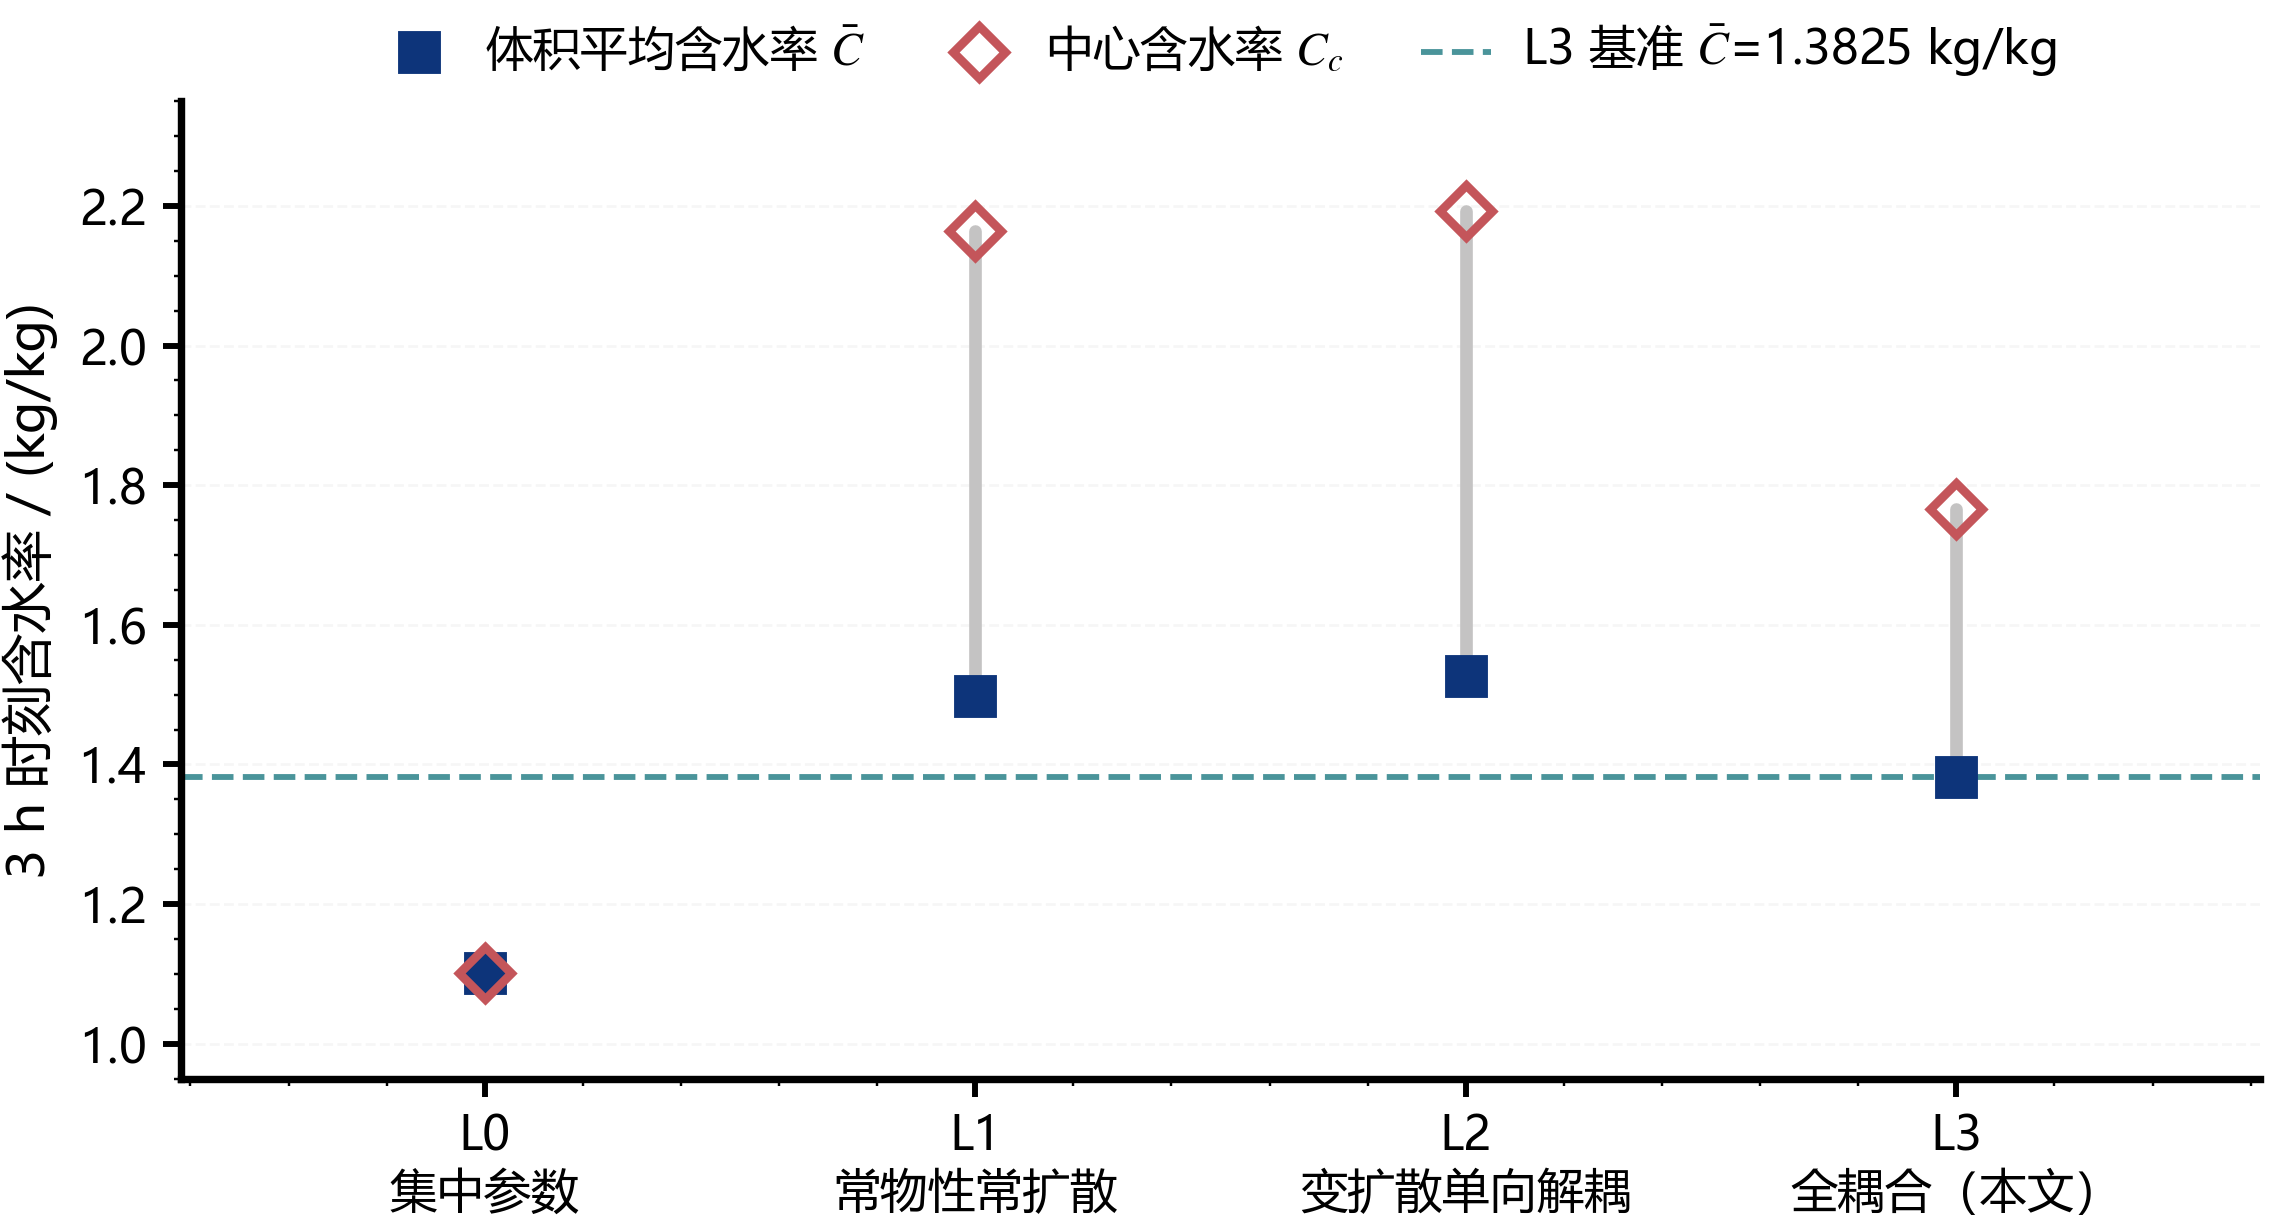
\includegraphics[width=0.90\textwidth]{figures/fig_q1_model_ladder.png}
  \caption[四级模型阶梯含水率指标对比]{四级模型阶梯在 3\,h 时刻的含水率指标棒棒糖对比：L0 集中参数、L1 常物性常扩散、L2 变扩散单向解耦、L3 全耦合（本文）。体积平均含水率依次为 1.1007/1.4986/1.5272/1.3825\,kg/kg，两两最小间隔 0.0286\,kg/kg（判据 $>10^{-6}$），确认四条路径为真实独立求解。L0 相对 L3 基准偏低 20.39\%，且其 $Bi_T$=1.3889、$Bi_m$=3.2404 均为 $O(1)$，故集中参数假设不成立，该路径仅作错误极限对照。}
  \label{fig:q1_model_ladder}
\end{figure}

\begin{figure}[H]
  \centering
  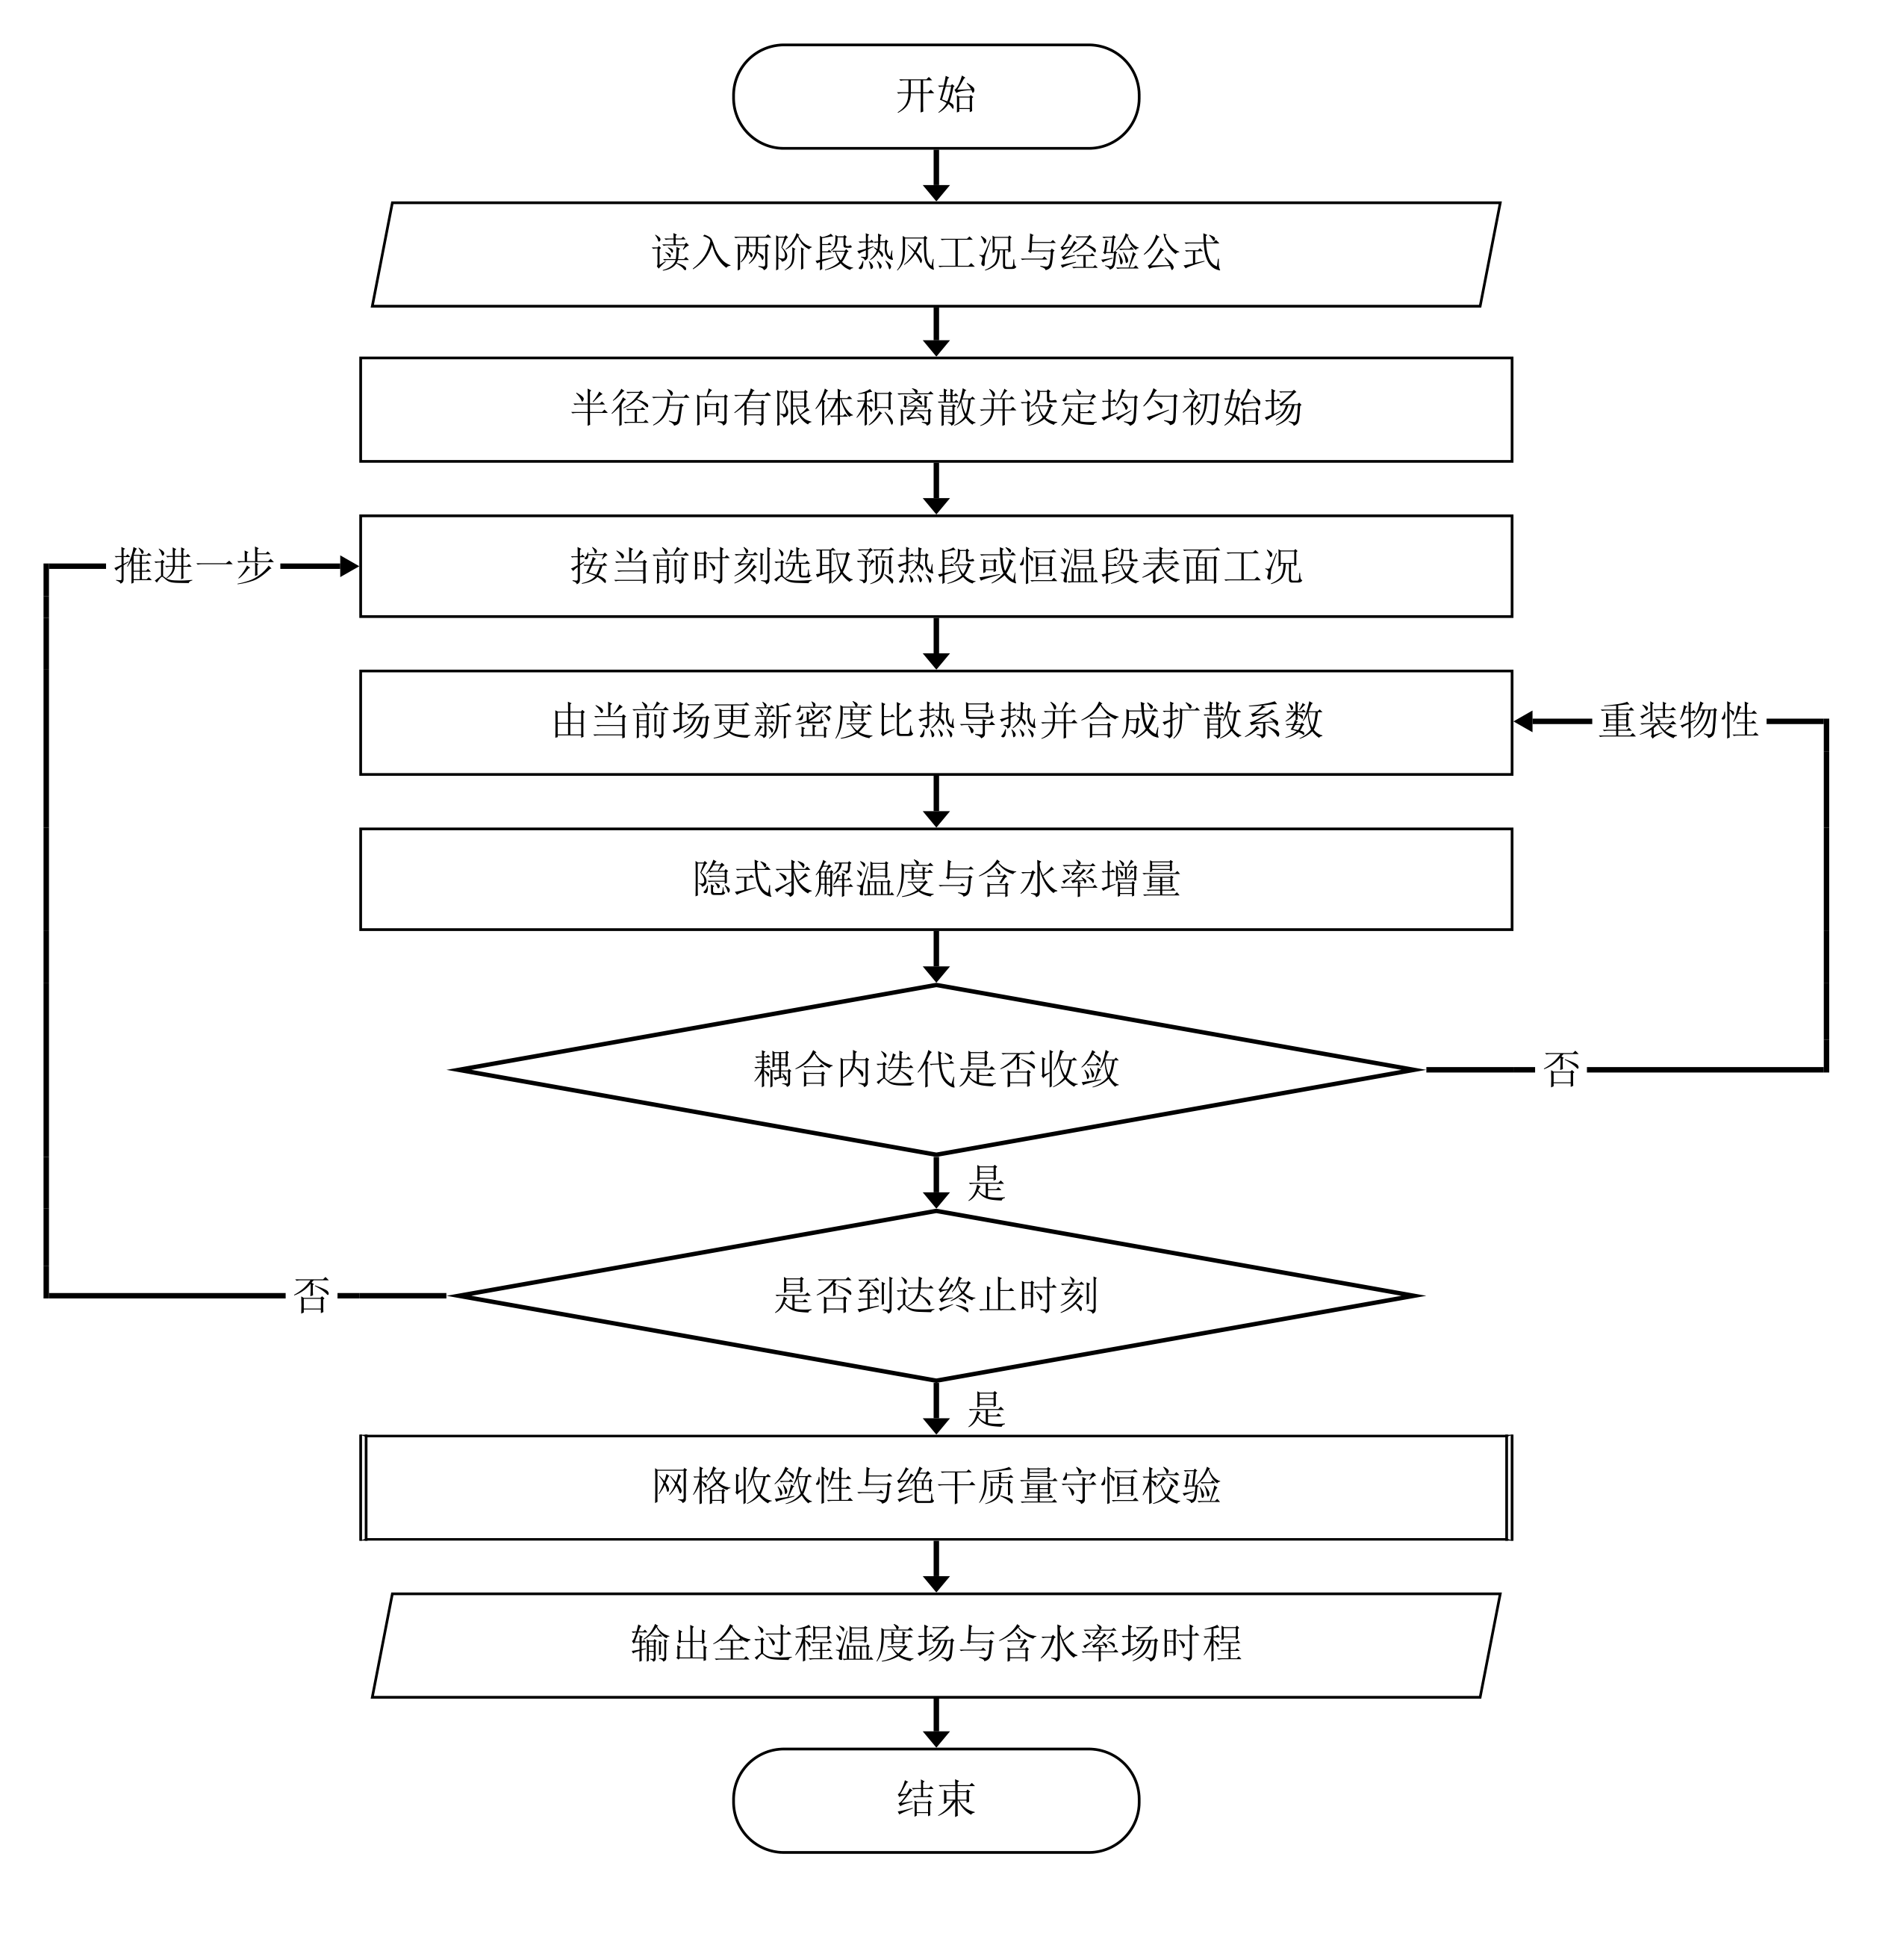
\includegraphics[width=0.95\textwidth]{figures/fig_flow_q2.png}
  \caption[问题二求解流程]{问题二求解流程。在问题一的温度场求解器上并联含水率方程，两场通过"温度抬升扩散系数"与"蒸发潜热回吸热量"双向耦合，每个时间步内交替求解并以耦合残差判断是否收敛；右侧回路为不收敛时的时间步细分。扩散系数取 $D(C,T)$ 的双因子形式，界面物性用调和平均以保证通量连续。}
  \label{fig:flow_q2}
\end{figure}

\begin{figure}[H]
  \centering
  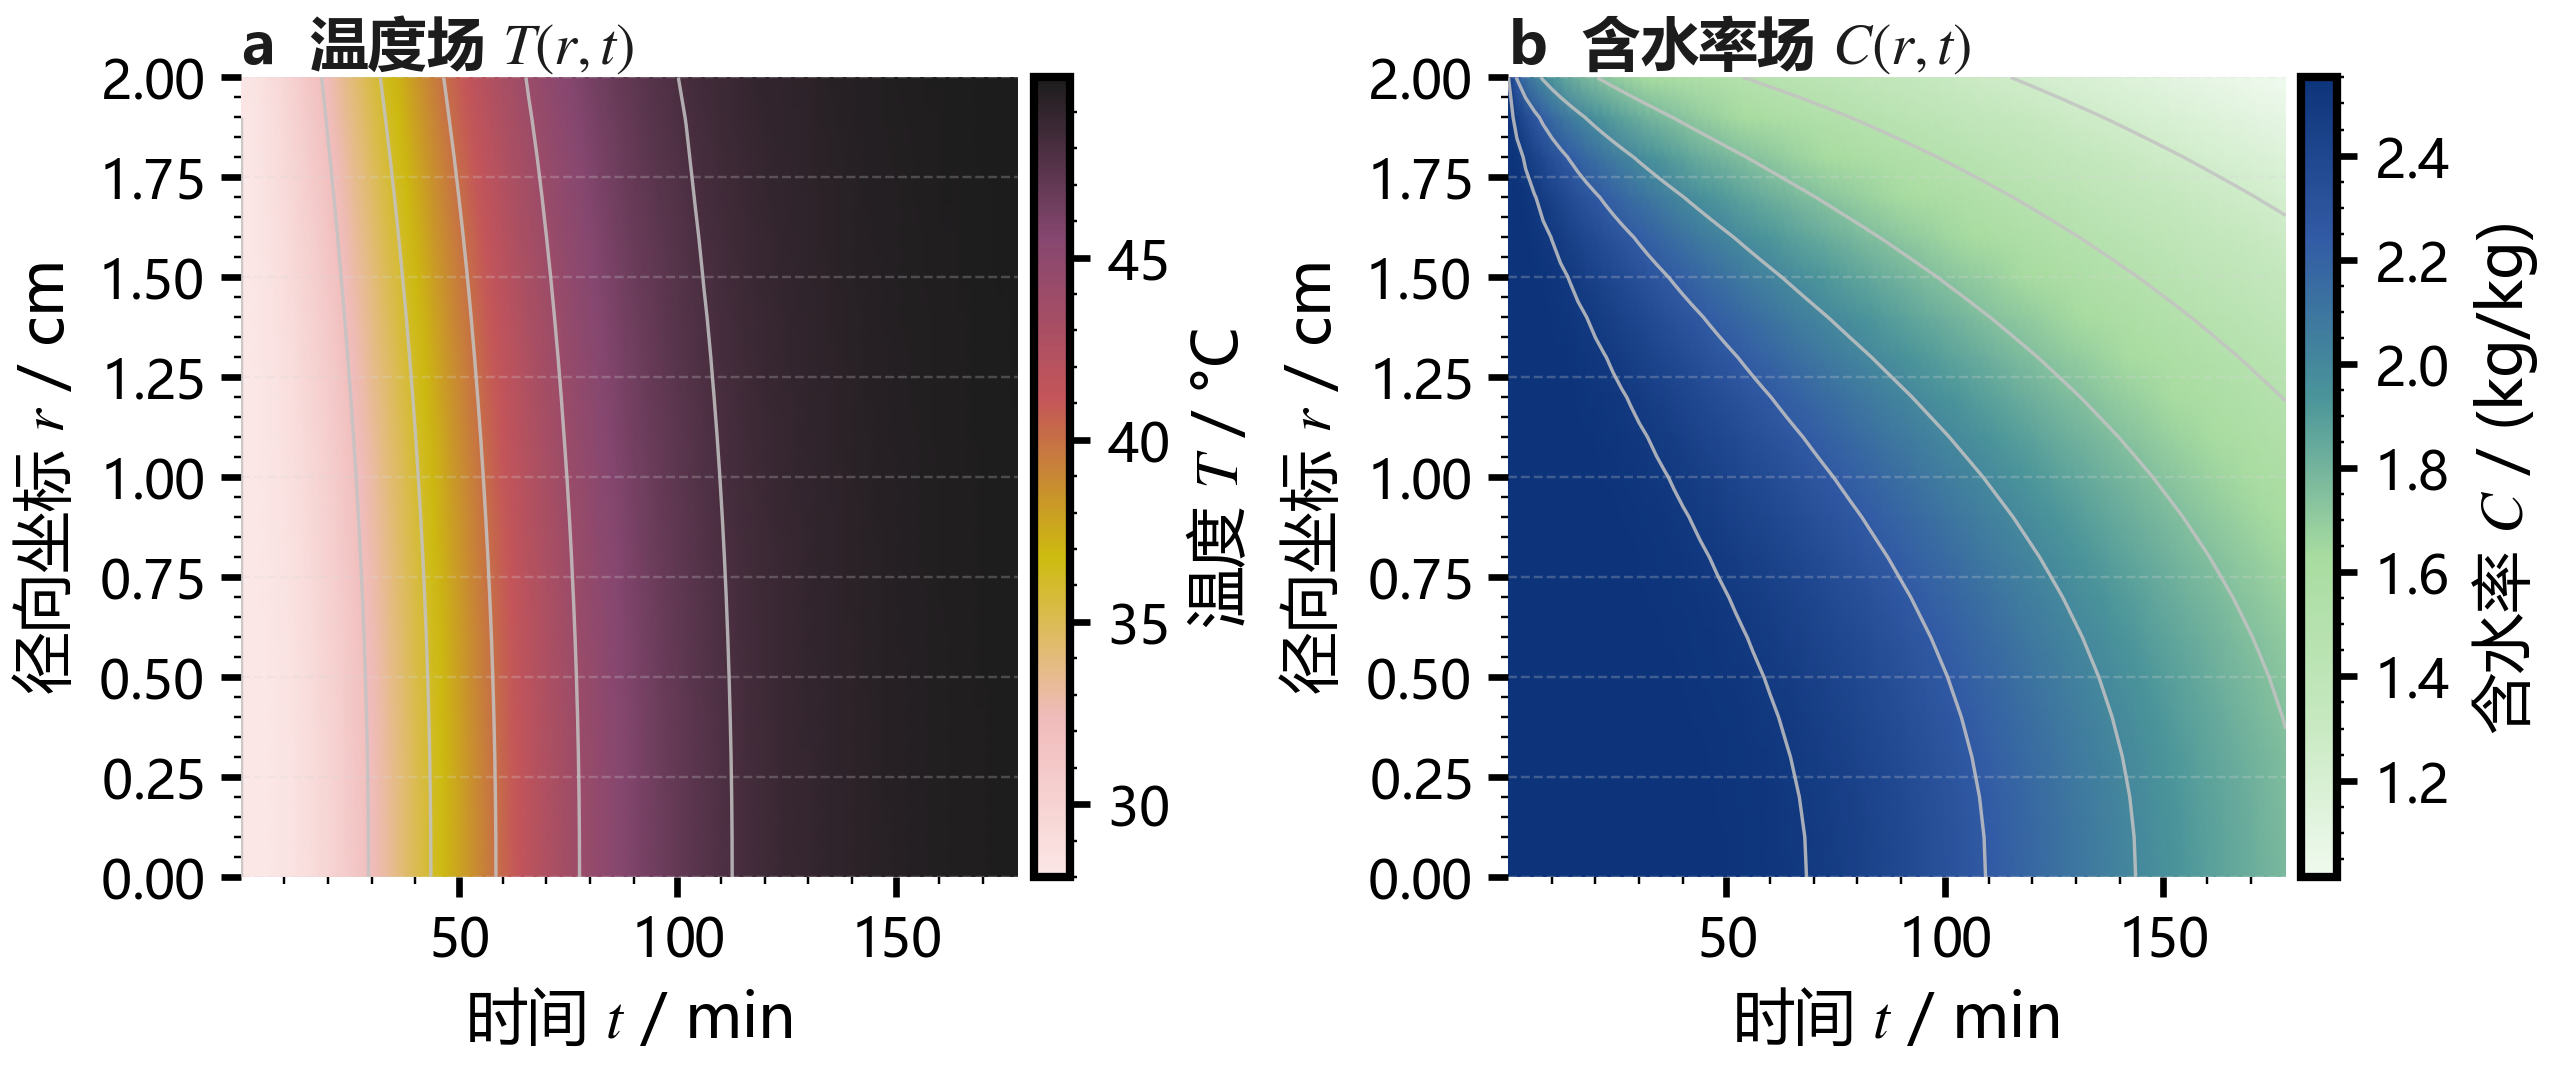
\includegraphics[width=1.00\textwidth]{figures/fig_q2_spacetime_heatmap.png}
  \caption[问题二温度场与含水率场时空热图]{问题二 3\,h 内温度场（面板 a）与含水率场（面板 b）的时空热图，纵轴为径向坐标、横轴为时间。温度在全域趋于一致，终态中心 49.849\,°C、表面 49.966\,°C，温差仅 0.117\,°C；含水率仍保持显著径向梯度，终态中心 1.7662、表面 1.0081\,kg/kg，体积平均 1.3825\,kg/kg。}
  \label{fig:q2_spacetime_heatmap}
\end{figure}

\begin{figure}[H]
  \centering
  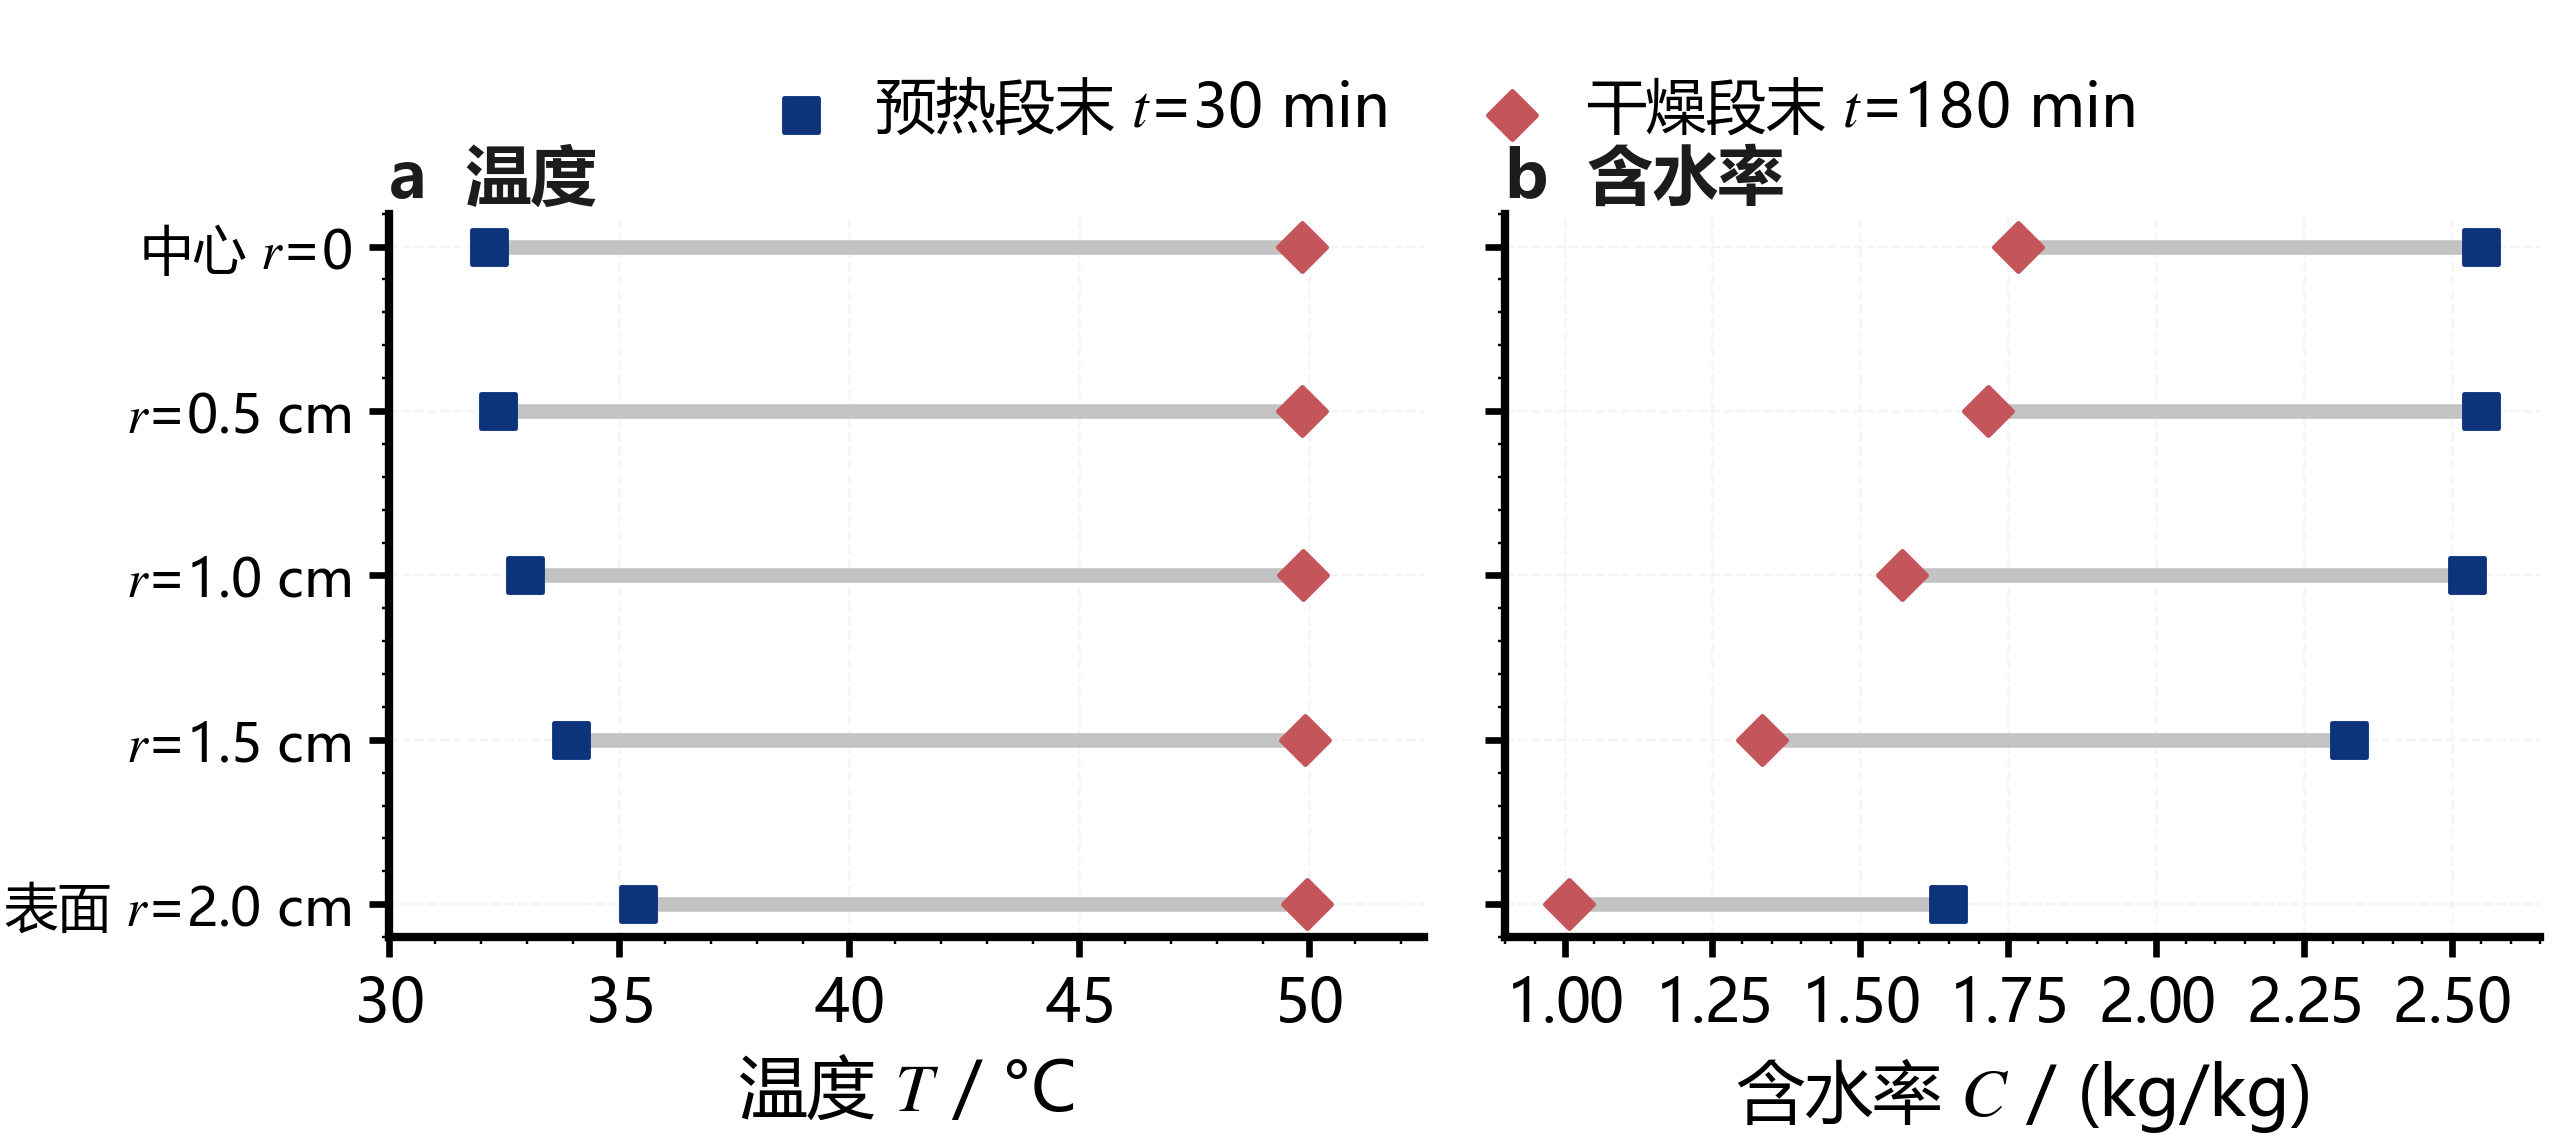
\includegraphics[width=1.00\textwidth]{figures/fig_q2_stage_compare.png}
  \caption[问题二预热段与恒温段哑铃对比]{问题二预热段与恒温干燥段的五测点哑铃对比，面板 a 为温度、b 为含水率。以 1800\,s 为分界：中心温度由 32.189\,°C 升至 49.849\,°C，中心含水率由 2.5499 降至 1.7662\,kg/kg，表面由 1.6486 降至 1.0081\,kg/kg。前段以升温为主、后段以失水为主，是恒温平台下驱动力切换的直接证据。}
  \label{fig:q2_stage_compare}
\end{figure}

\begin{figure}[H]
  \centering
  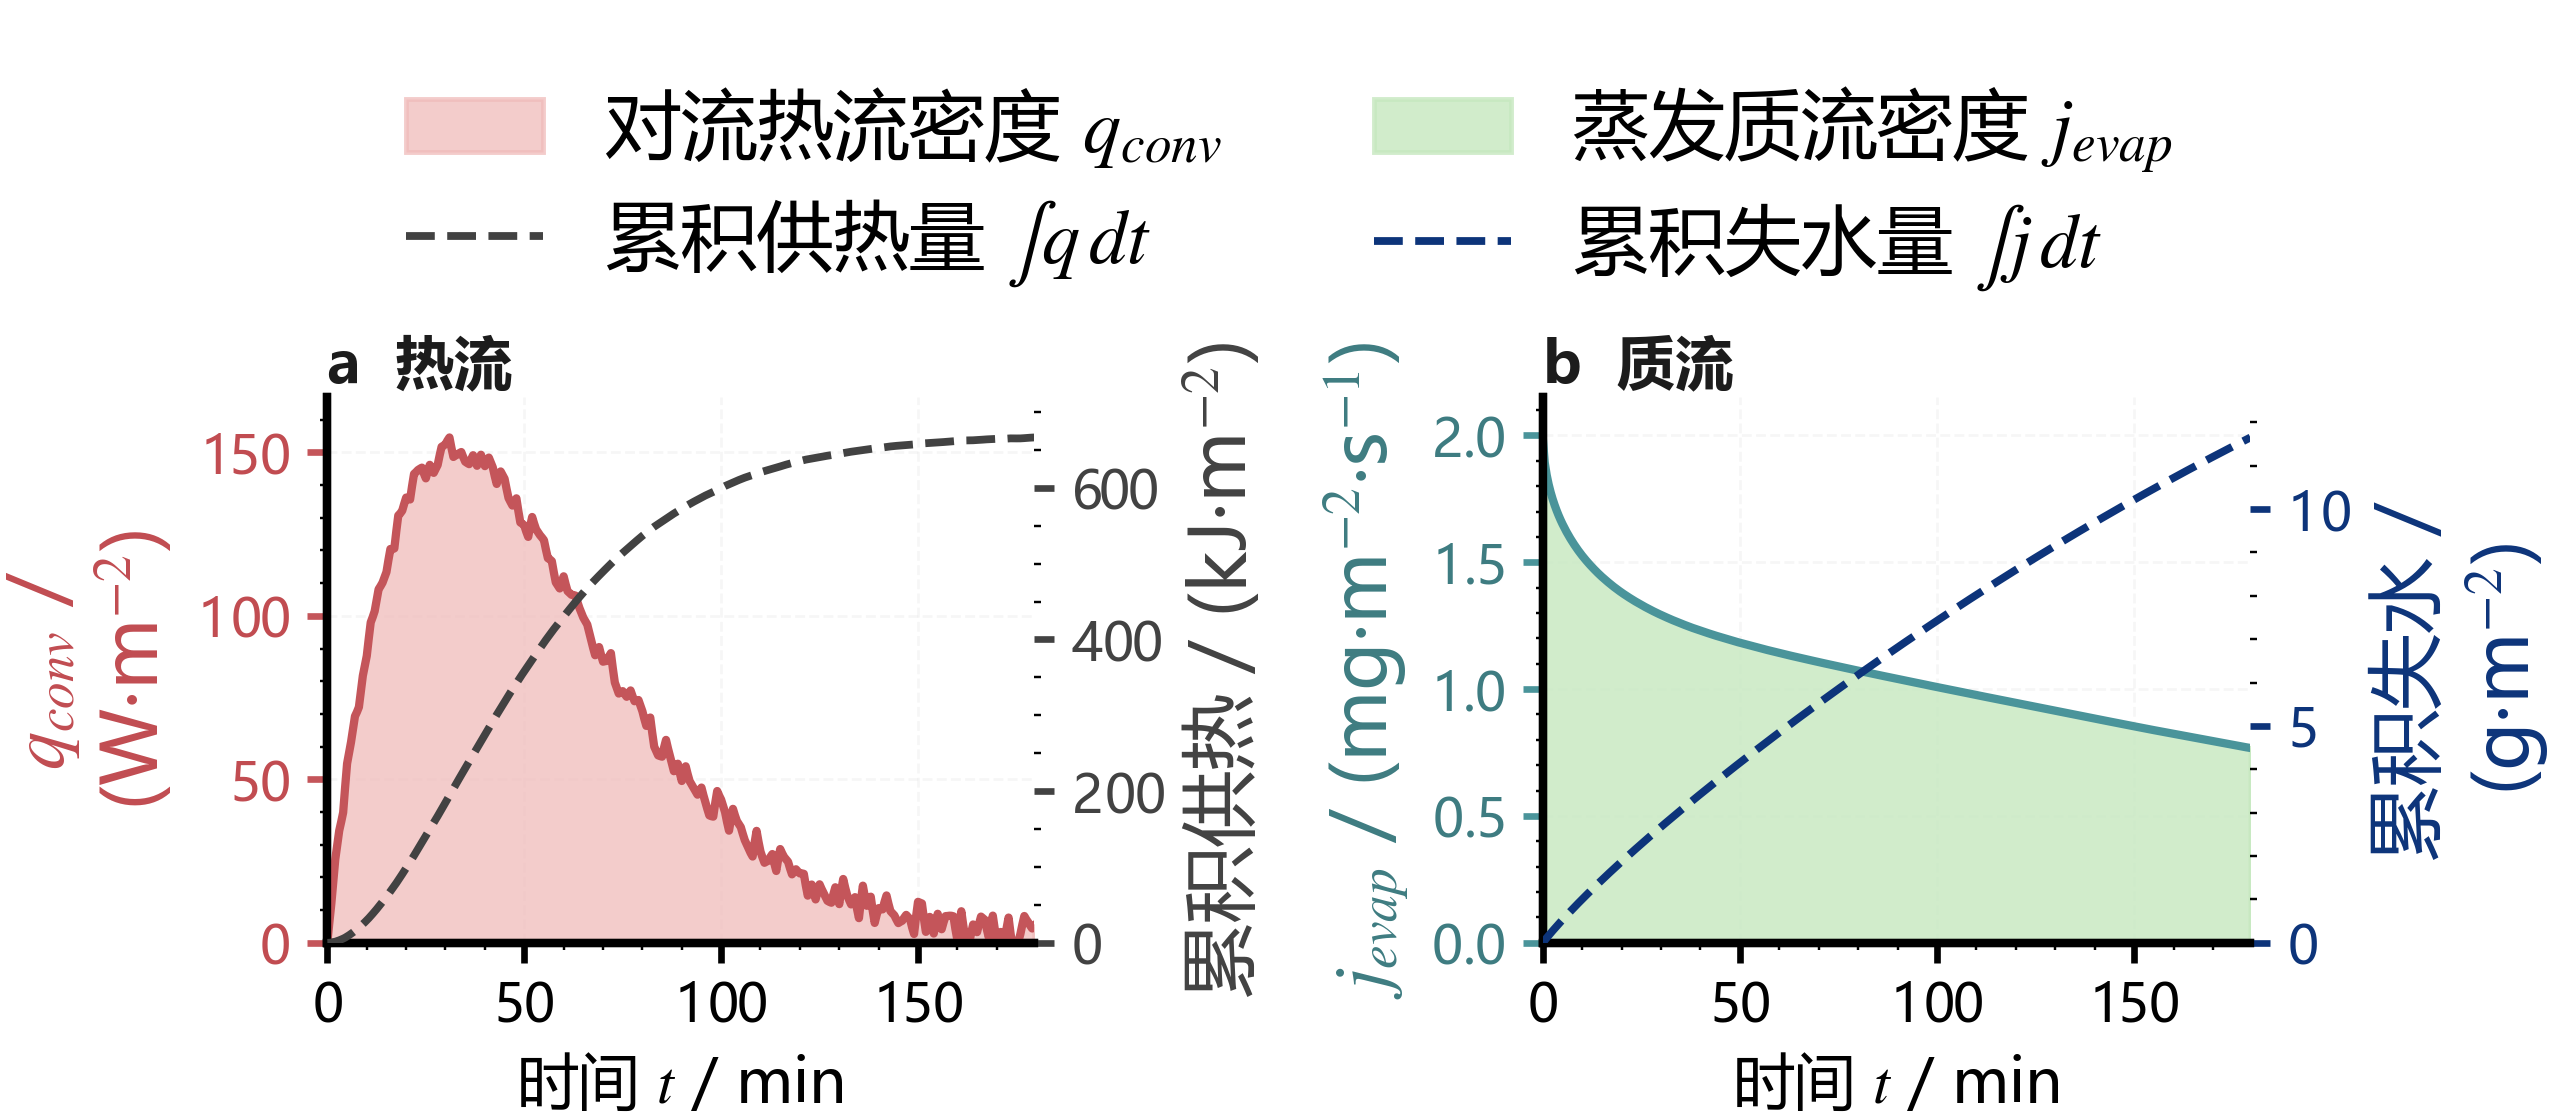
\includegraphics[width=1.00\textwidth]{figures/fig_q2_coupling_flux.png}
  \caption[问题二表面热流与蒸发质流时程]{问题二表面对流热流（面板 a）与蒸发质流（面板 b）的面积时程，量化热--质耦合强度。热流随表面温度接近热风温度而衰减，质流则受表面含水率下降与扩散系数上升共同支配；扩散系数由 $t$=0 的 $5.642\times10^{-9}$ 升至终态中心 $1.239\times10^{-8}$\,m$^2$/s（增至 2.20 倍）。}
  \label{fig:q2_coupling_flux}
\end{figure}

\begin{figure}[H]
  \centering
  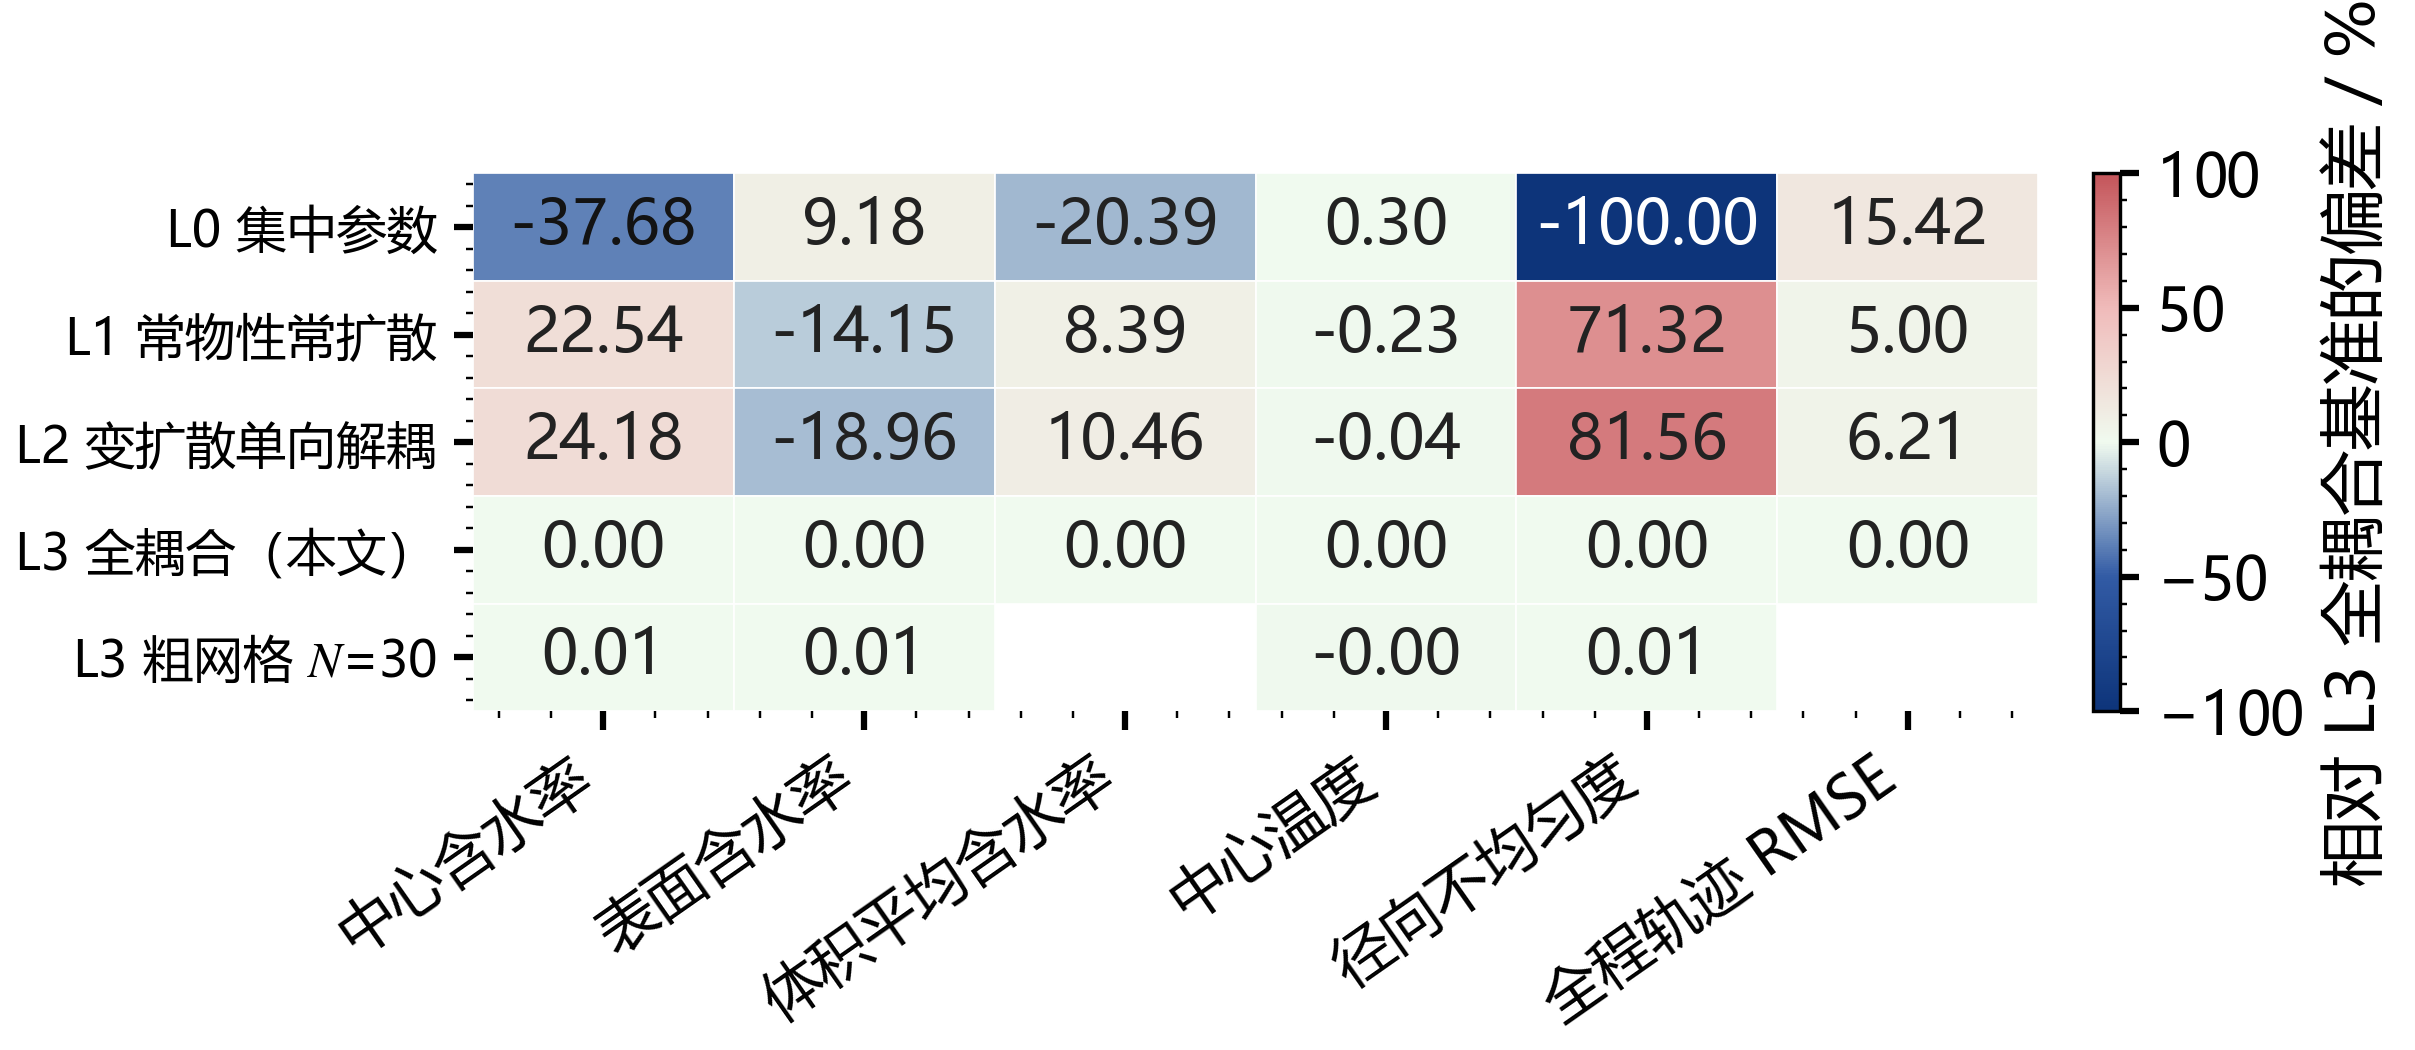
\includegraphics[width=0.98\textwidth]{figures/fig_q2_model_compare.png}
  \caption[四级模型阶梯方法对比热图]{四级模型阶梯与 L3 粗网格（$N$=30）共五行、六项指标的方法对比热图，色标为相对 L3 全耦合基准的相对偏差。建模误差远大于离散误差：L0 在中心含水率上偏离 -37.68\%、L1 偏离 22.54\%、L2 偏离 24.18\%，而 L3 粗网格仅偏离 0.0074\%。\emph{体积平均含水率} 与 \emph{全程轨迹 RMSE} 两列对粗网格行留空，因该档阶梯未输出对应量，按缺测处理而非以零填充。}
  \label{fig:q2_model_compare}
\end{figure}

\begin{figure}[H]
  \centering
  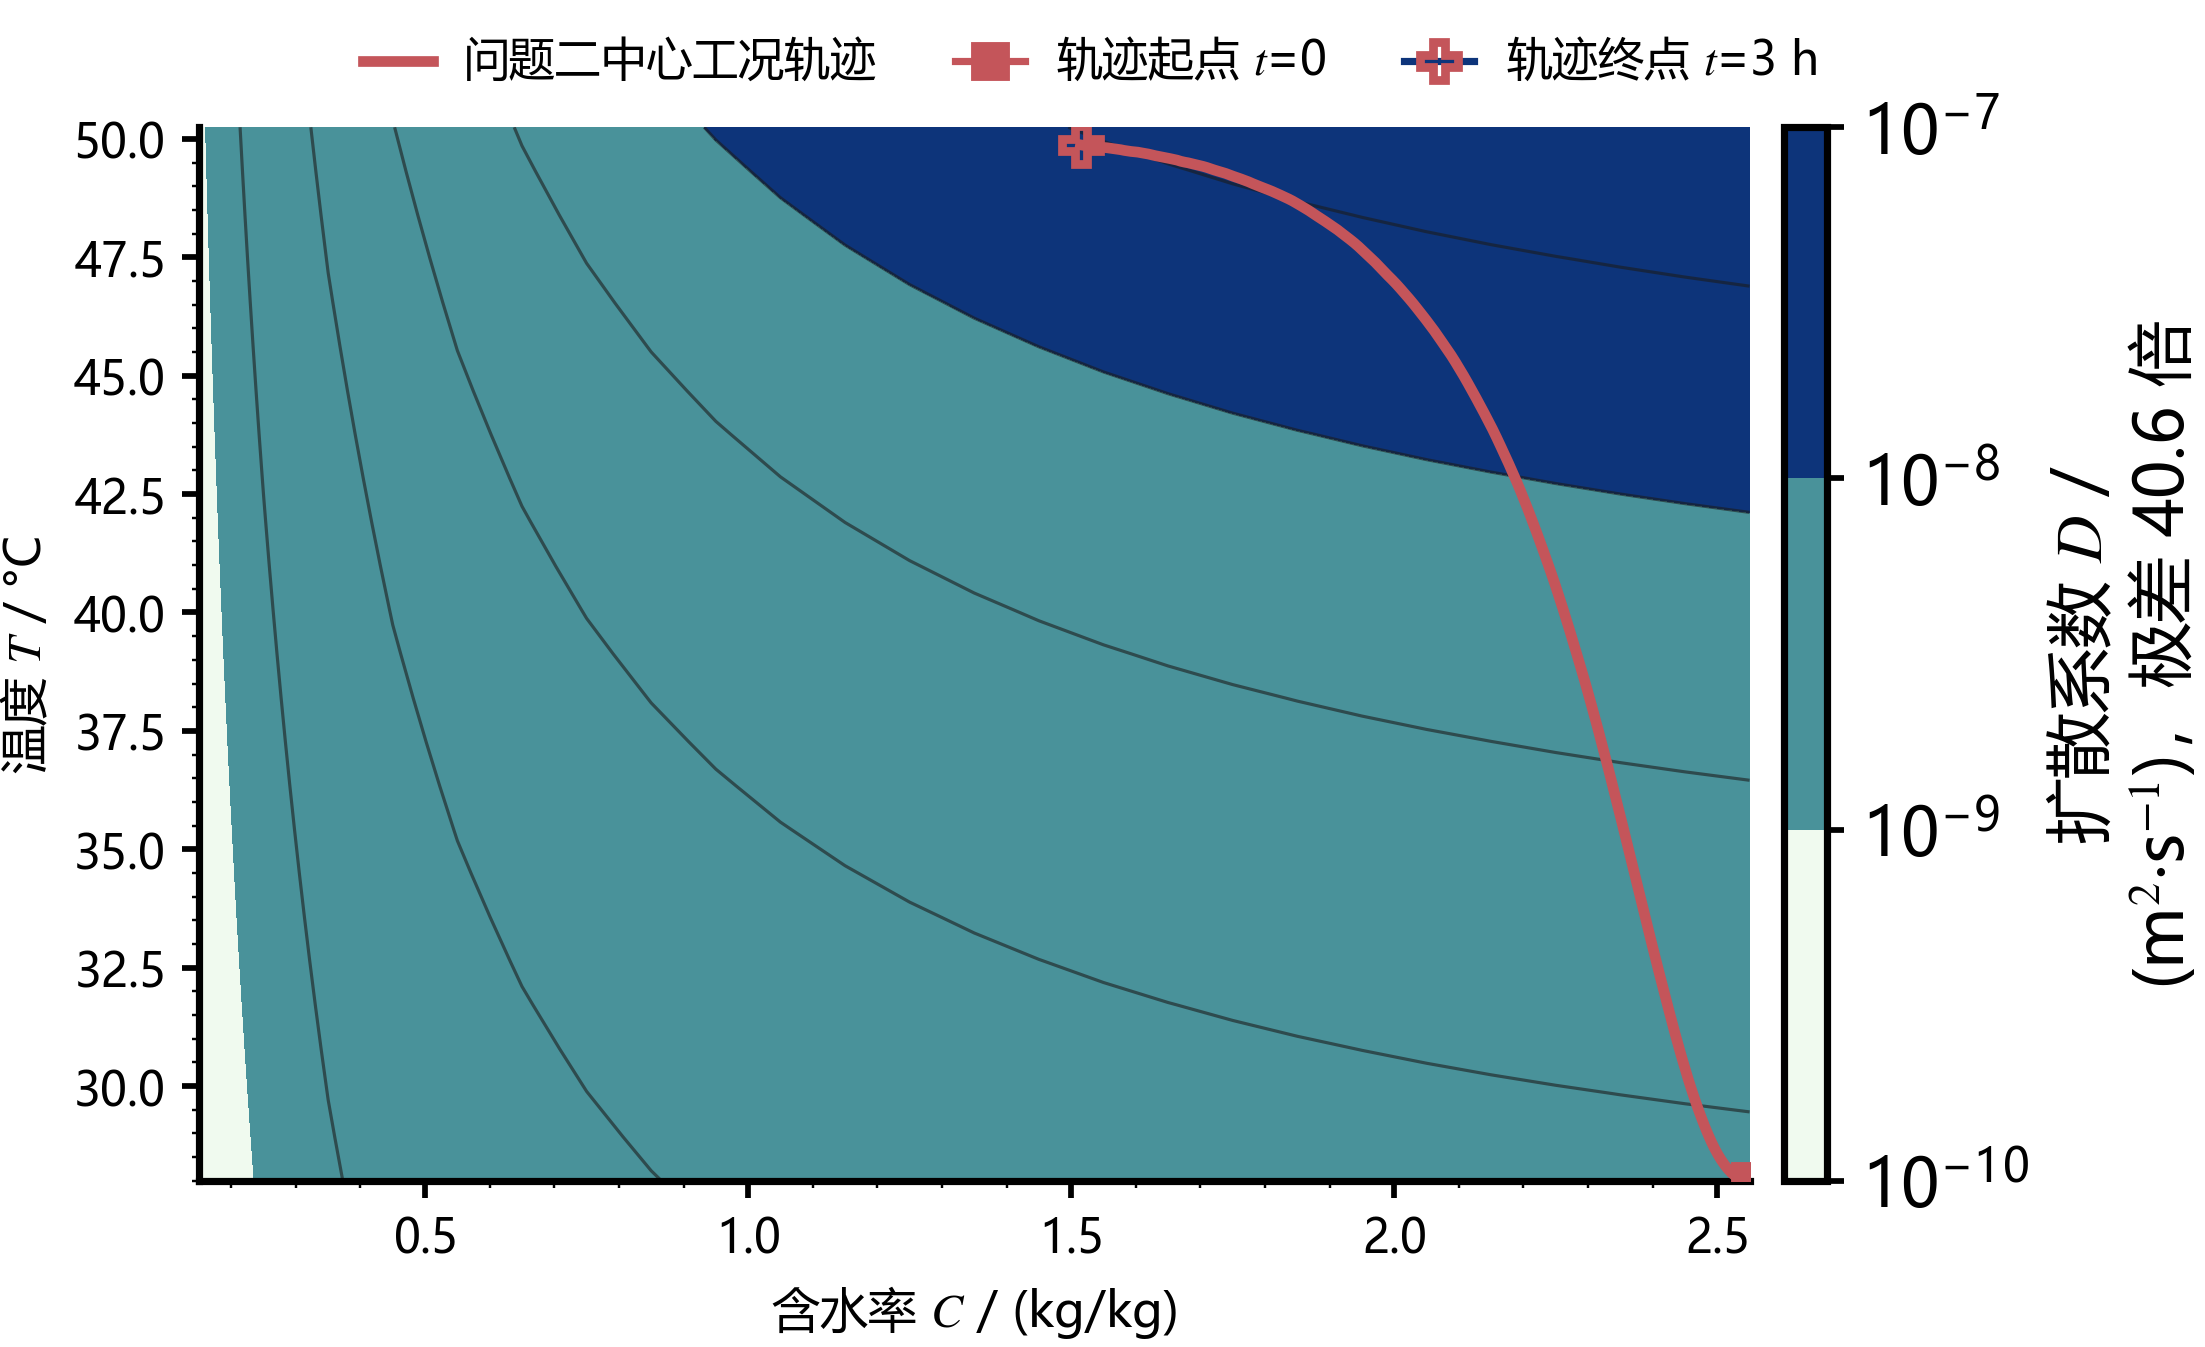
\includegraphics[width=0.90\textwidth]{figures/fig_q2_D_response_surface.png}
  \caption[扩散系数 $D(C,T)$ 等值线与工况轨迹]{扩散系数 $D(C,T)$ 的等值线填充图，白色轨迹为问题二实际工况在 $(C,T)$ 平面上的走向。网格范围内 $D$ 自 $3.351\times10^{-10}$ 变到 $1.359\times10^{-8}$\,m$^2$/s，极差达 40.6 倍。$D$ 随温度升高而增大、随含水率下降而减小，两者在烘干过程中反向抵消，故轨迹在色带间近似横穿而非顺色梯度下滑。}
  \label{fig:q2_D_response_surface}
\end{figure}

\begin{figure}[H]
  \centering
  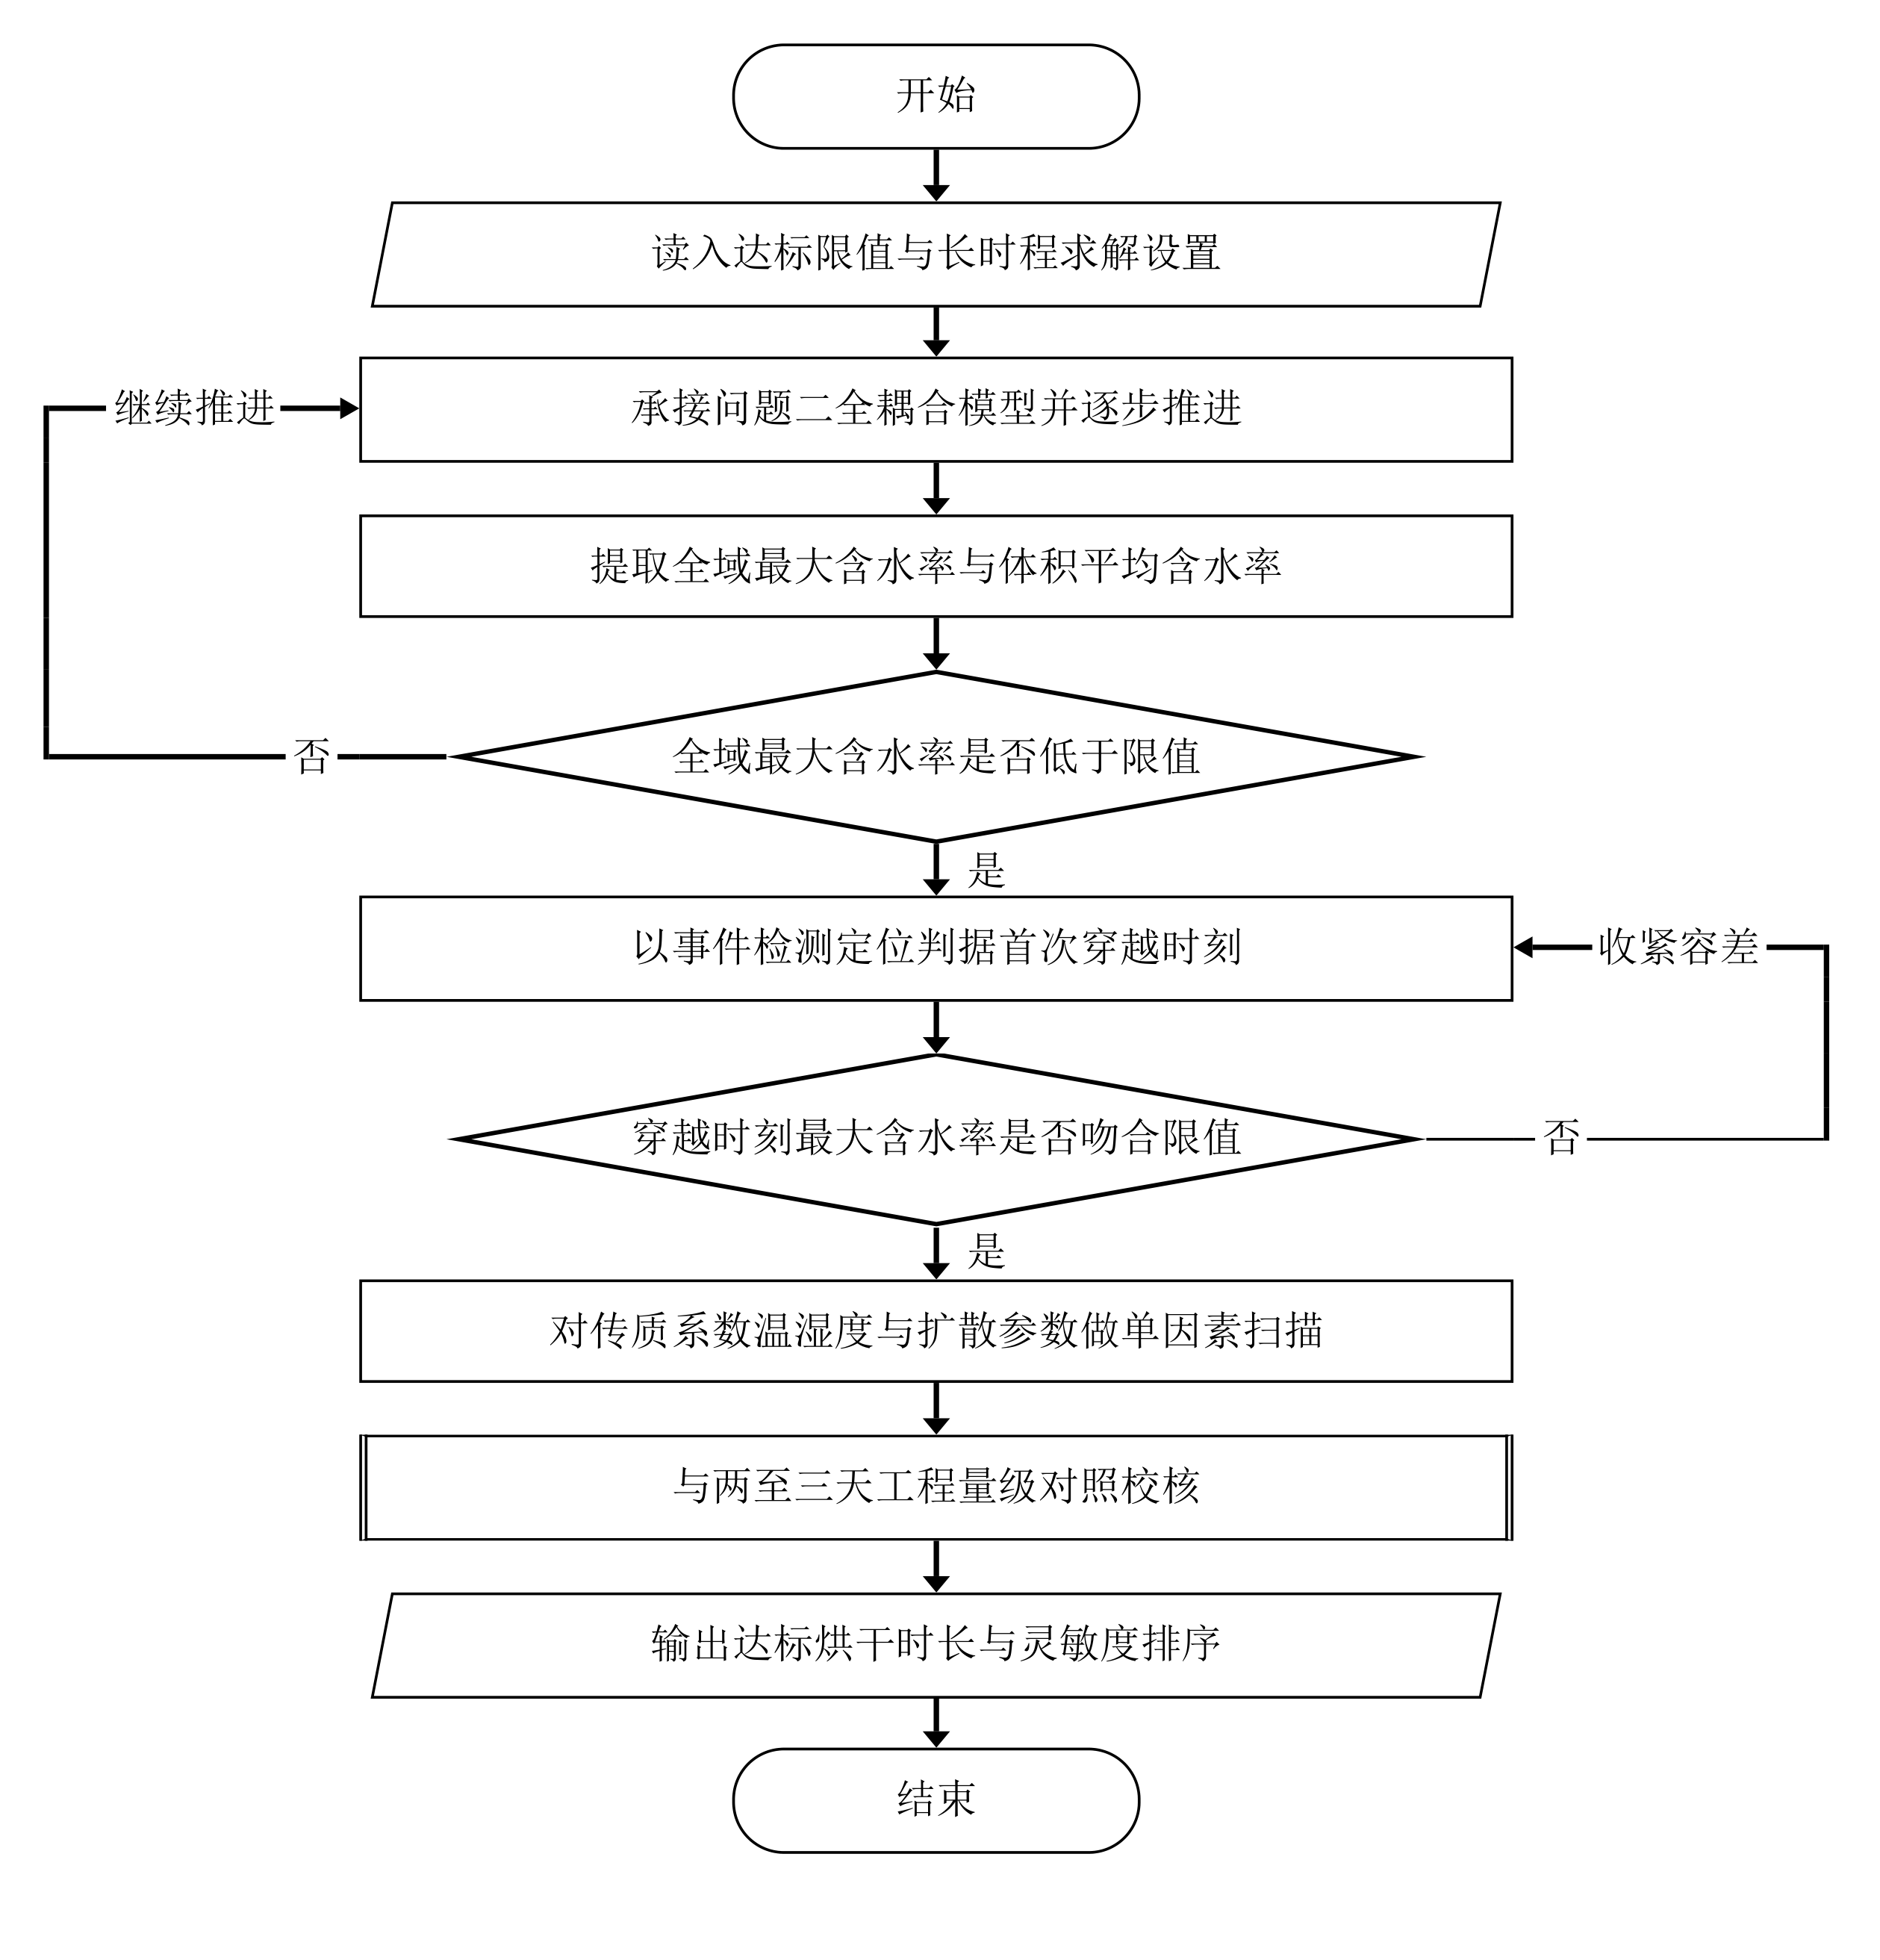
\includegraphics[width=0.95\textwidth]{figures/fig_flow_q3.png}
  \caption[问题三求解流程]{问题三求解流程。沿用问题二的耦合求解器推进到含水率判据满足，判据满足性在每步末检验，未达标则继续推进、达标则记录时刻；随后进入敏感度分支：单因子扰动给出排序，拉丁超立方抽样给出秩相关，两者一致方接受结论。左侧回路为容差收紧后的重算。}
  \label{fig:flow_q3}
\end{figure}

\begin{figure}[H]
  \centering
  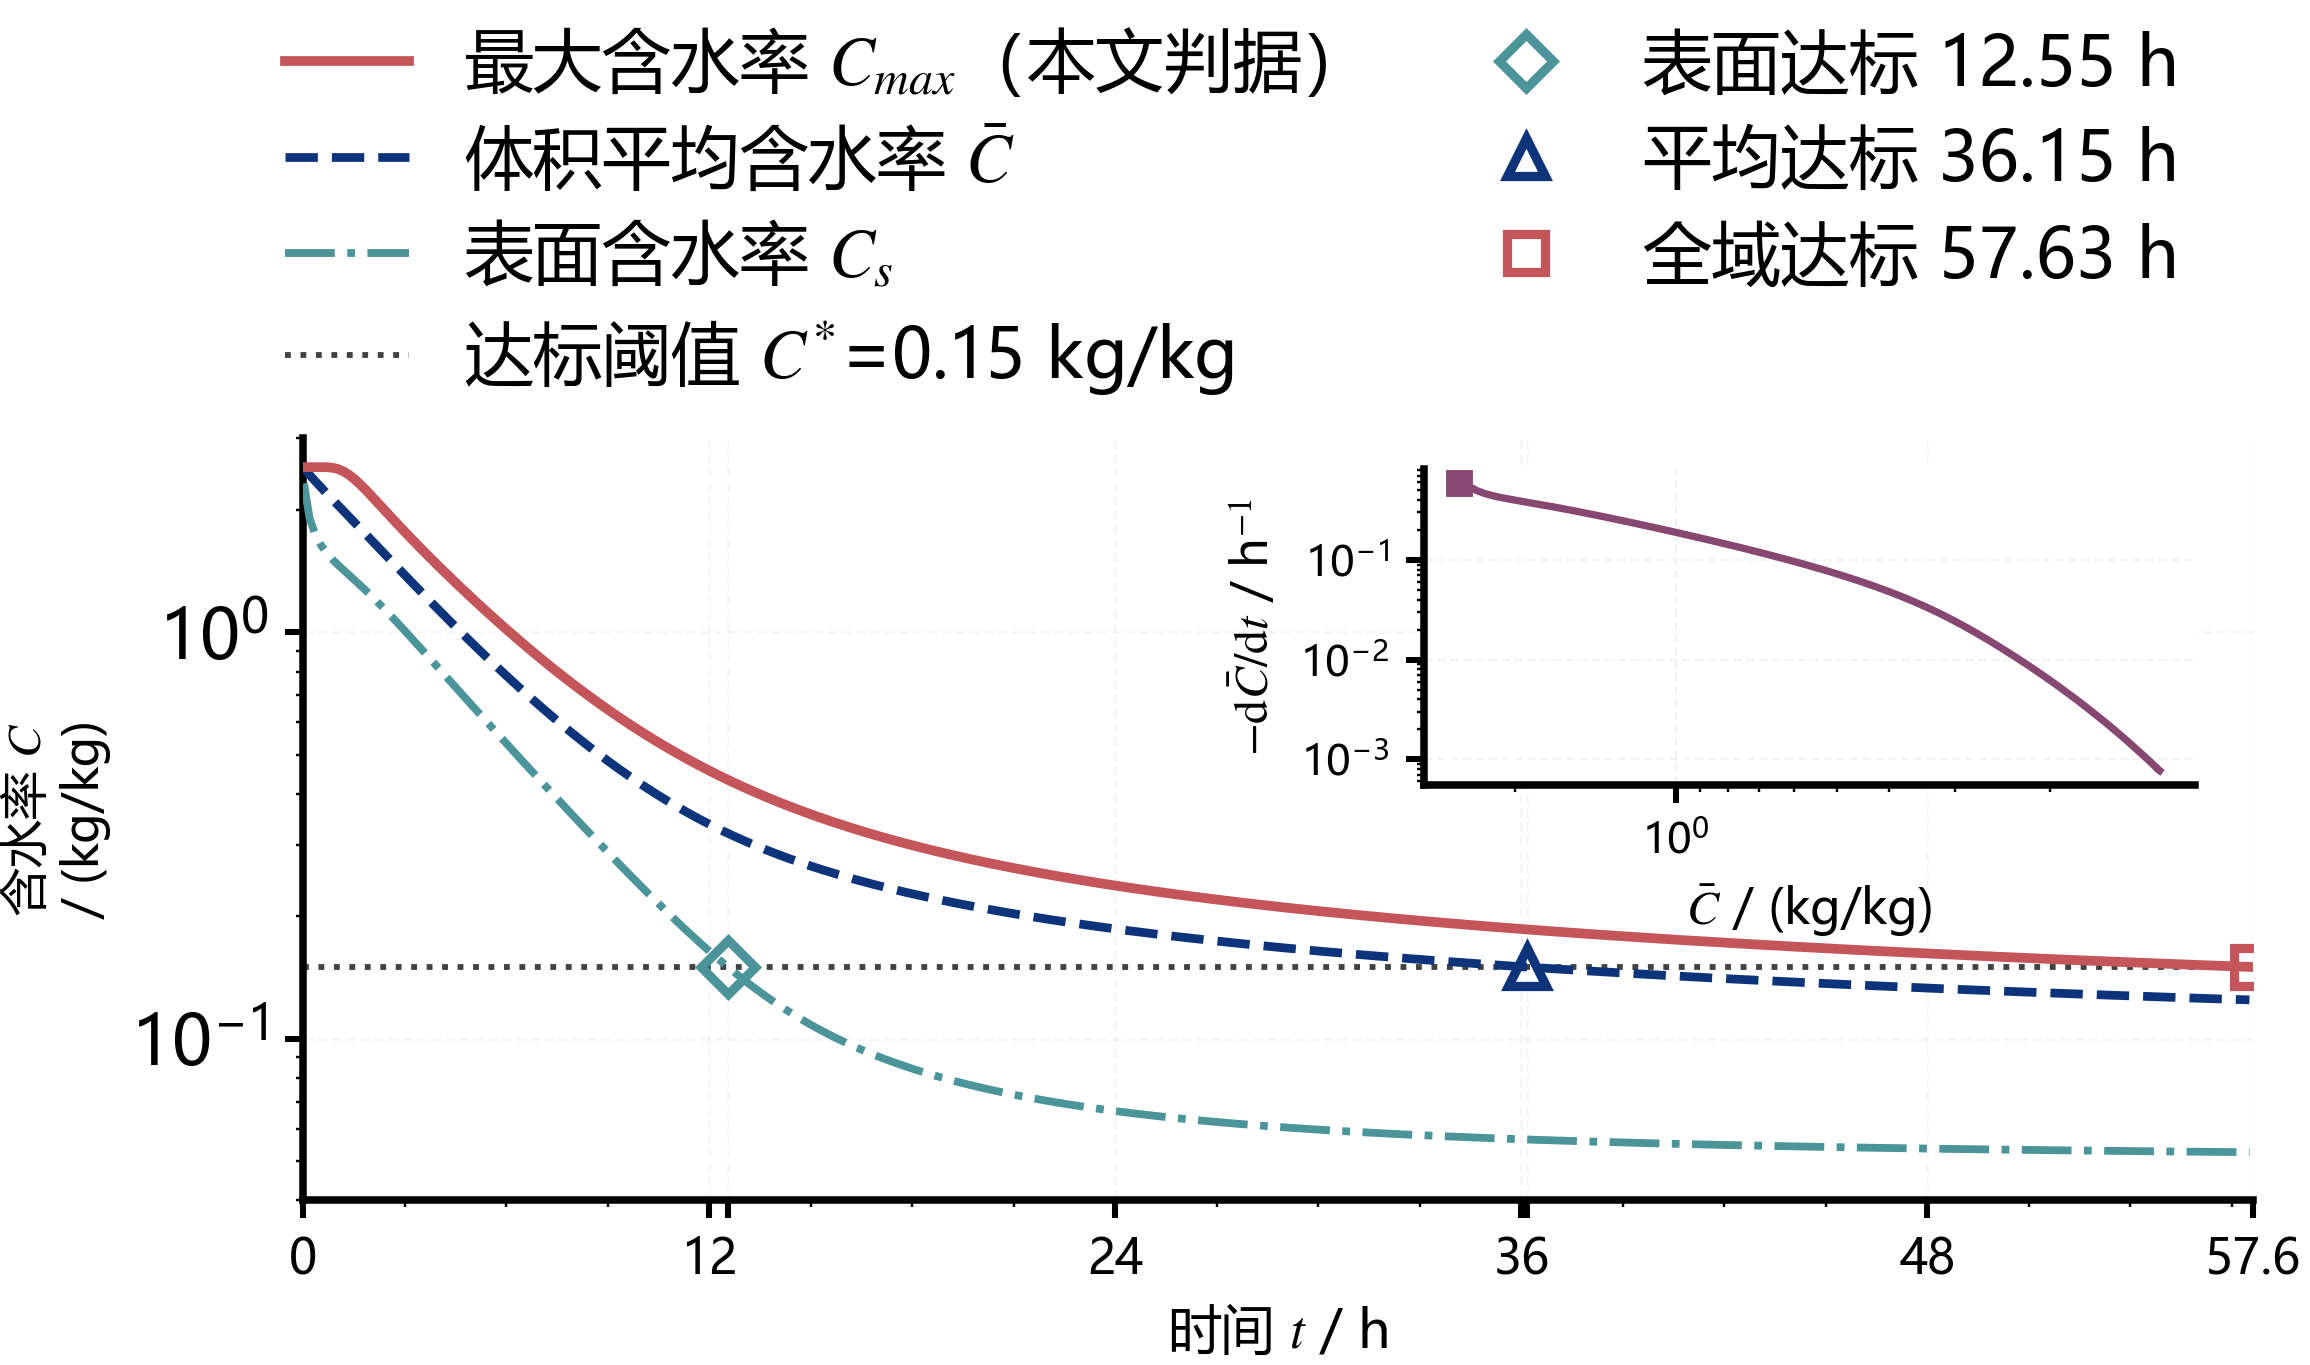
\includegraphics[width=0.92\textwidth]{figures/fig_q3_drying_curve.png}
  \caption[问题三全程干燥曲线与达标时刻]{问题三全程干燥曲线：最大值、体积平均、中心、表面四条含水率轨迹与 $C^{*}$=0.15\,kg/kg 阈值线，竖线为达标时刻。以最保守的场内最大值为判据，$t_{end}$=57.625\,h（2.401\,d）；此刻中心 0.1500、表面 0.0525、体积平均 0.1244\,kg/kg。终点处最大含水率与阈值的间隙 0（判据 $<10^{-5}$），确认事件检测精确命中。}
  \label{fig:q3_drying_curve}
\end{figure}

\begin{figure}[H]
  \centering
  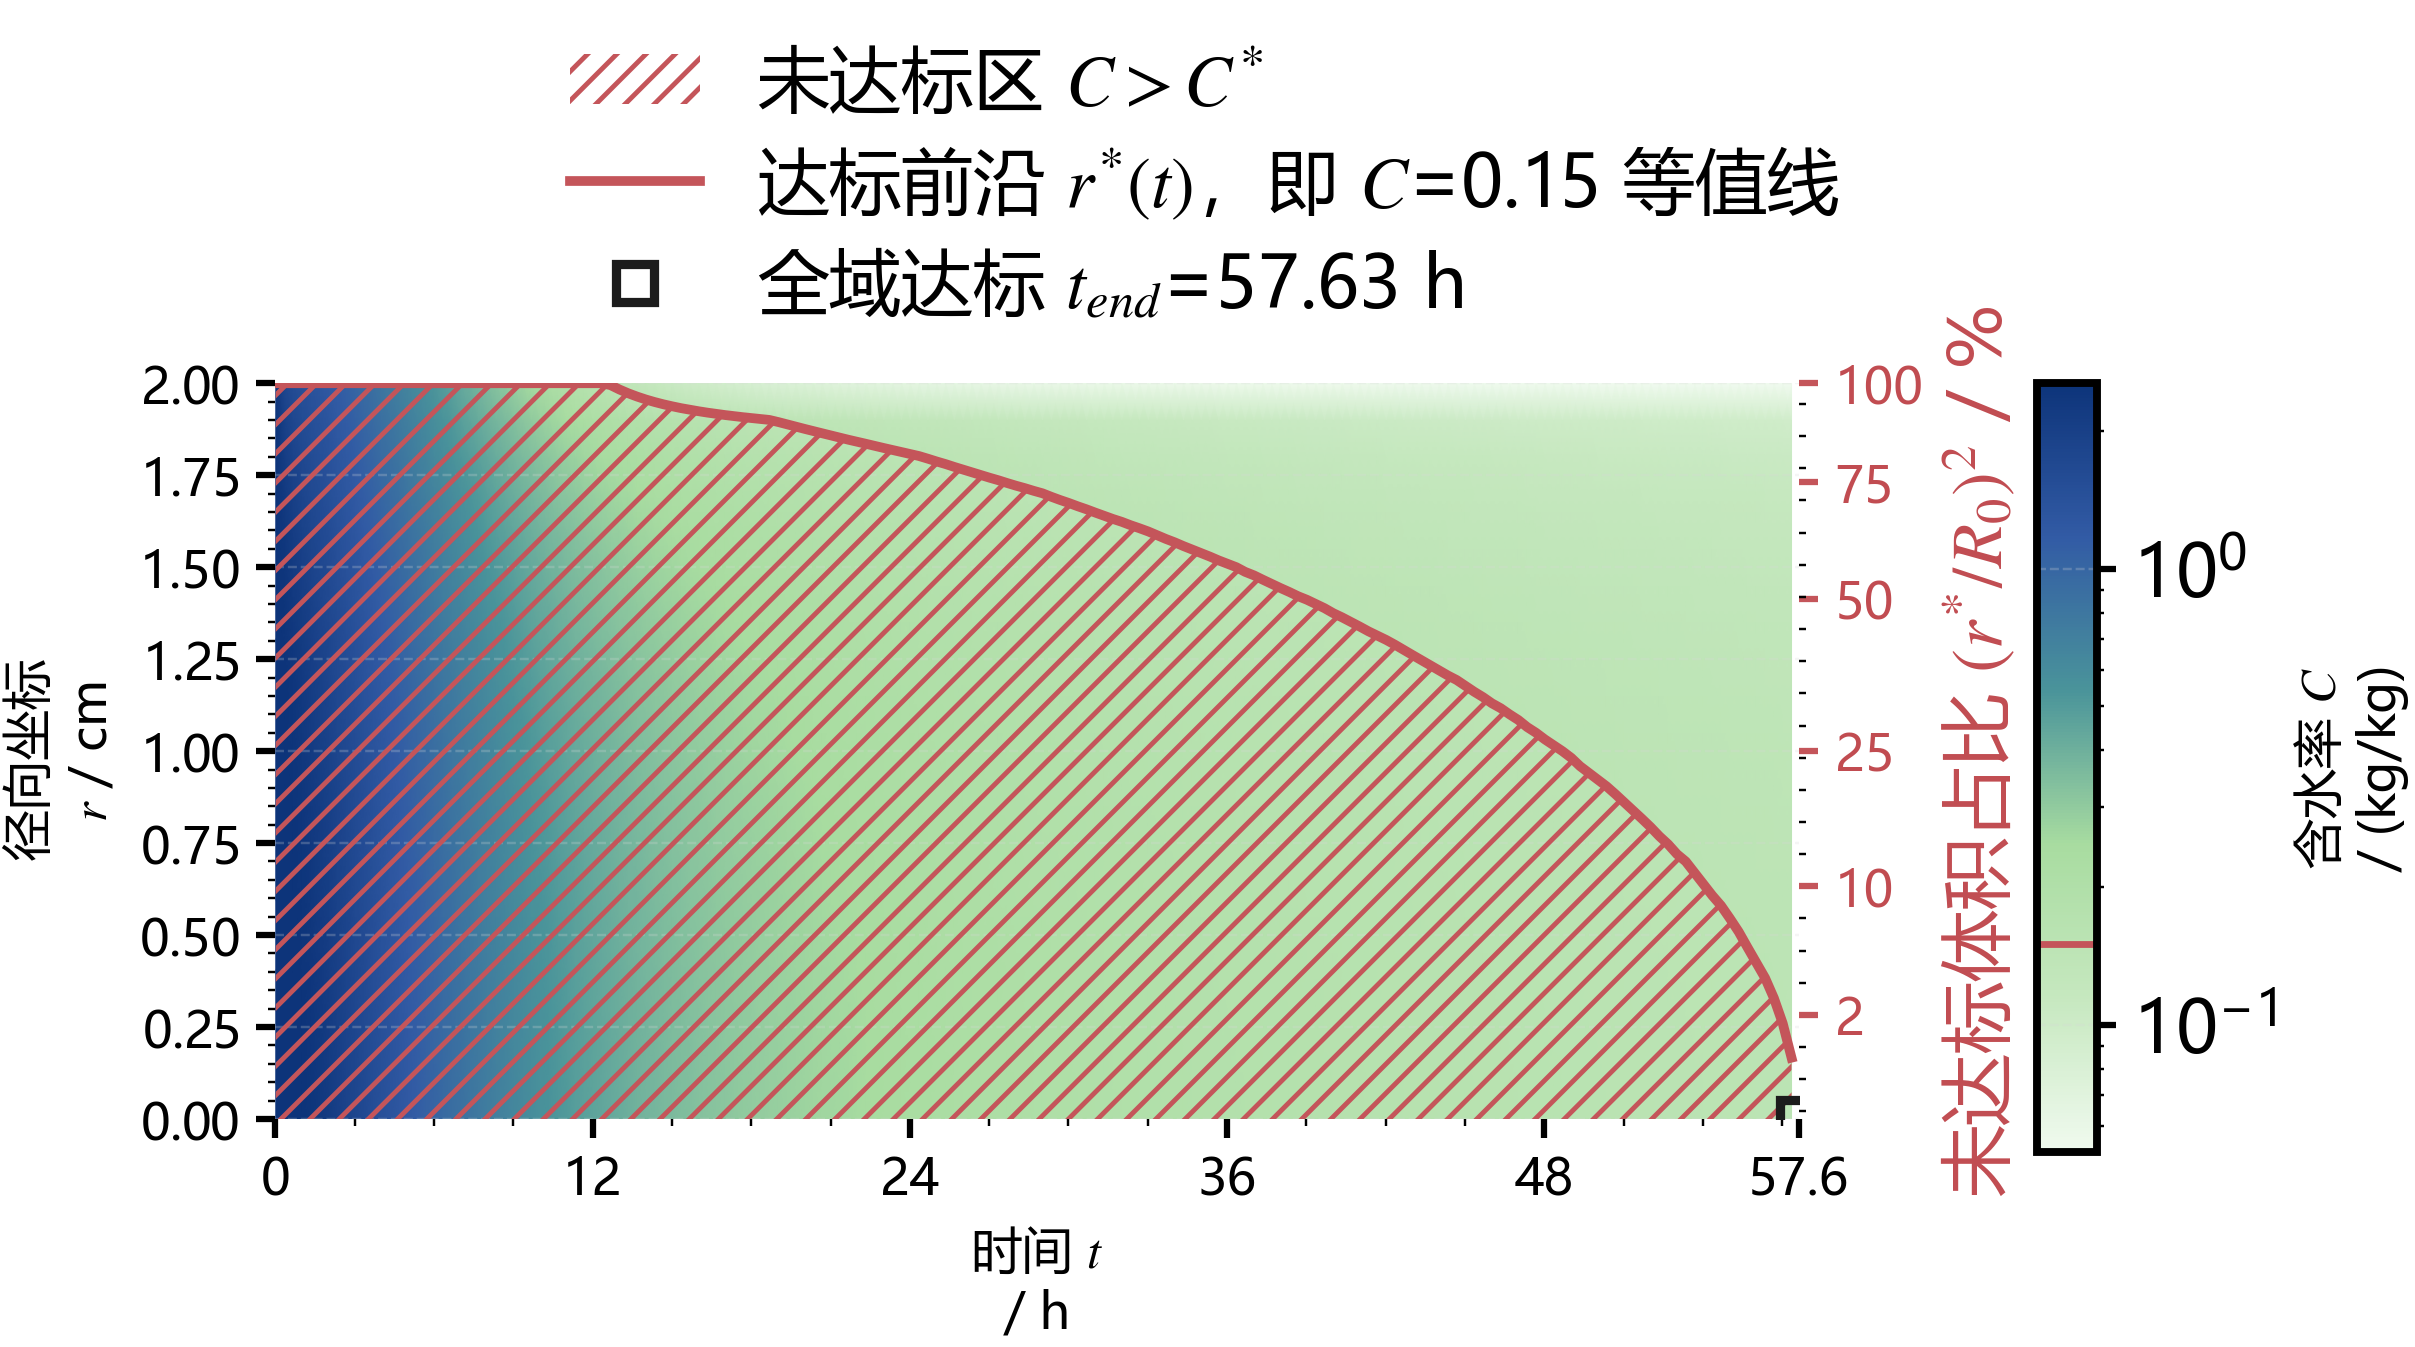
\includegraphics[width=0.94\textwidth]{figures/fig_q3_threshold_map.png}
  \caption[问题三达标时空图与未达标区收缩]{问题三达标时空图：$C(r,t)$ 云图叠加 $C^{*}$=0.15\,kg/kg 等值线，阴影为未达标区。达标前沿 $r^{*}(t)$ 自表面向中心推进，右轴同步给出未达标体积占比 $(r^{*}/R_0)^2$，圆柱几何下两者一一对应。中心为最后达标点（判据校验：最大含水率始终出现在中心单元），全域达标于 $t_{end}$=57.625\,h。}
  \label{fig:q3_threshold_map}
\end{figure}

\begin{figure}[H]
  \centering
  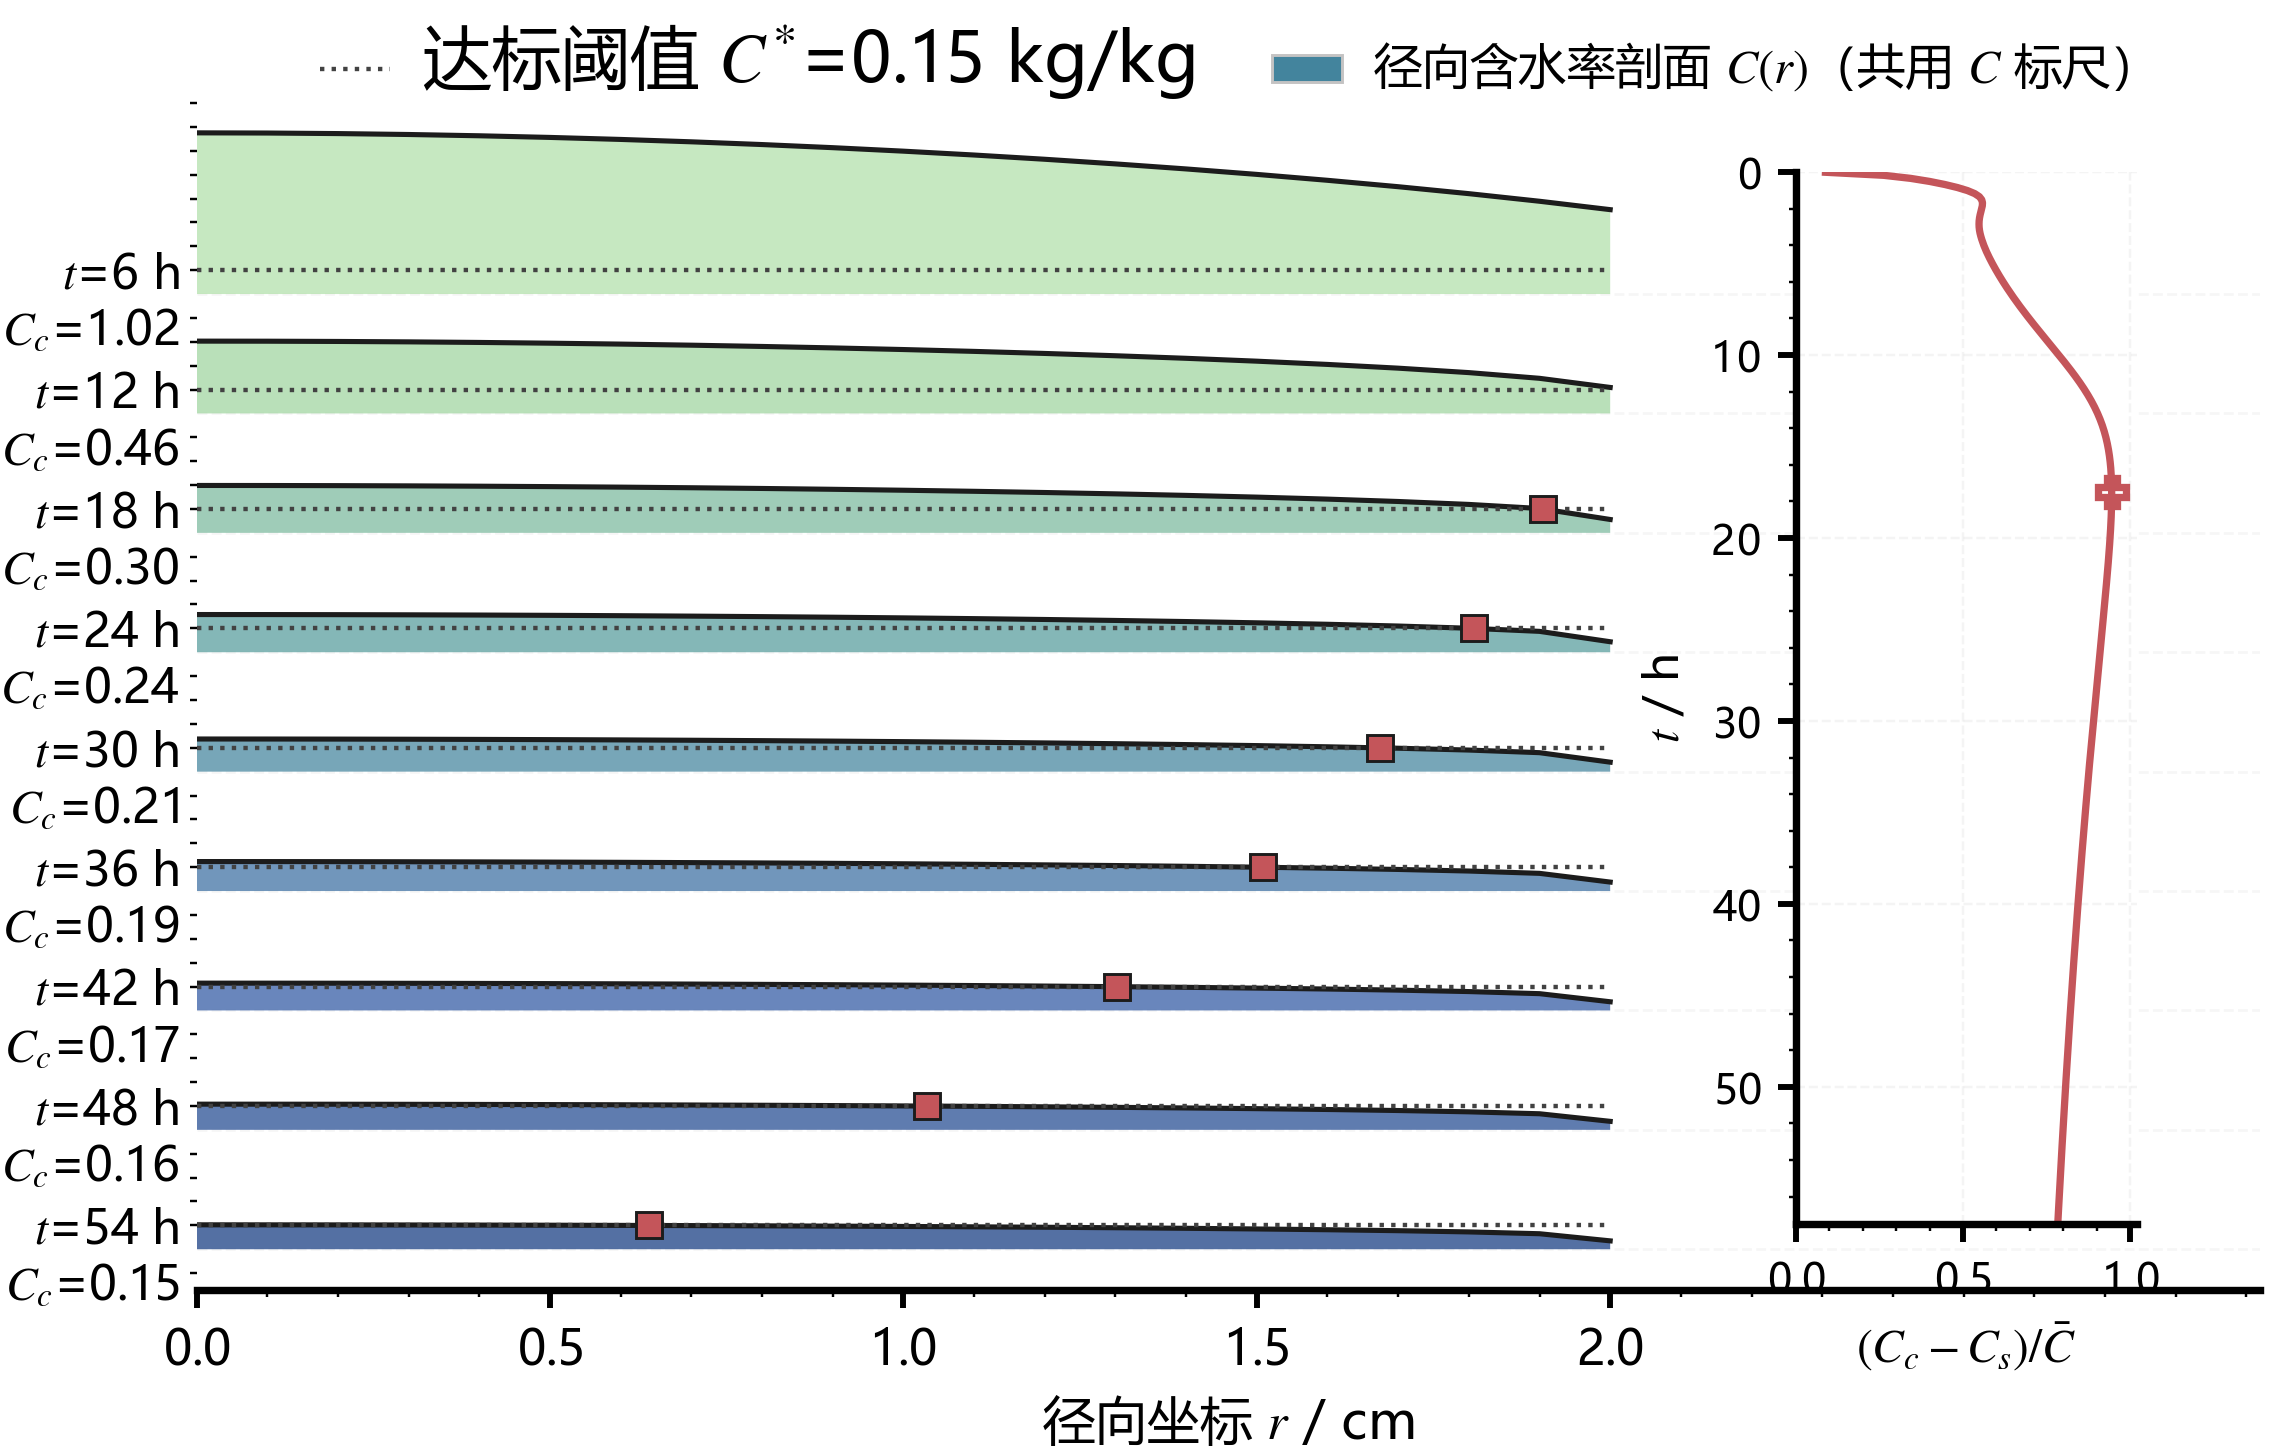
\includegraphics[width=0.92\textwidth]{figures/fig_q3_uniformity.png}
  \caption[问题三径向含水率剖面山脊线]{问题三 9 个时刻（6/12/18/24/30/36/42/48/54\,h）径向含水率剖面的山脊线图，各脊共用同一 $C$ 标尺，点线为 $C^{*}$=0.15\,kg/kg，红点为该时刻的达标前沿 $r^{*}$。中心含水率自 1.017 降至 0.154\,kg/kg，表面同期由 0.533 降至 0.053\,kg/kg。插图为相对不均匀度 $(C_c-C_s)/\bar{C}$ 的时间过程（时间轴向下、与脊序同向），在 $t$=17.52\,h 达峰值 0.945 后回落至 0.784，即径向不均匀先加剧后趋缓。}
  \label{fig:q3_uniformity}
\end{figure}

\begin{figure}[H]
  \centering
  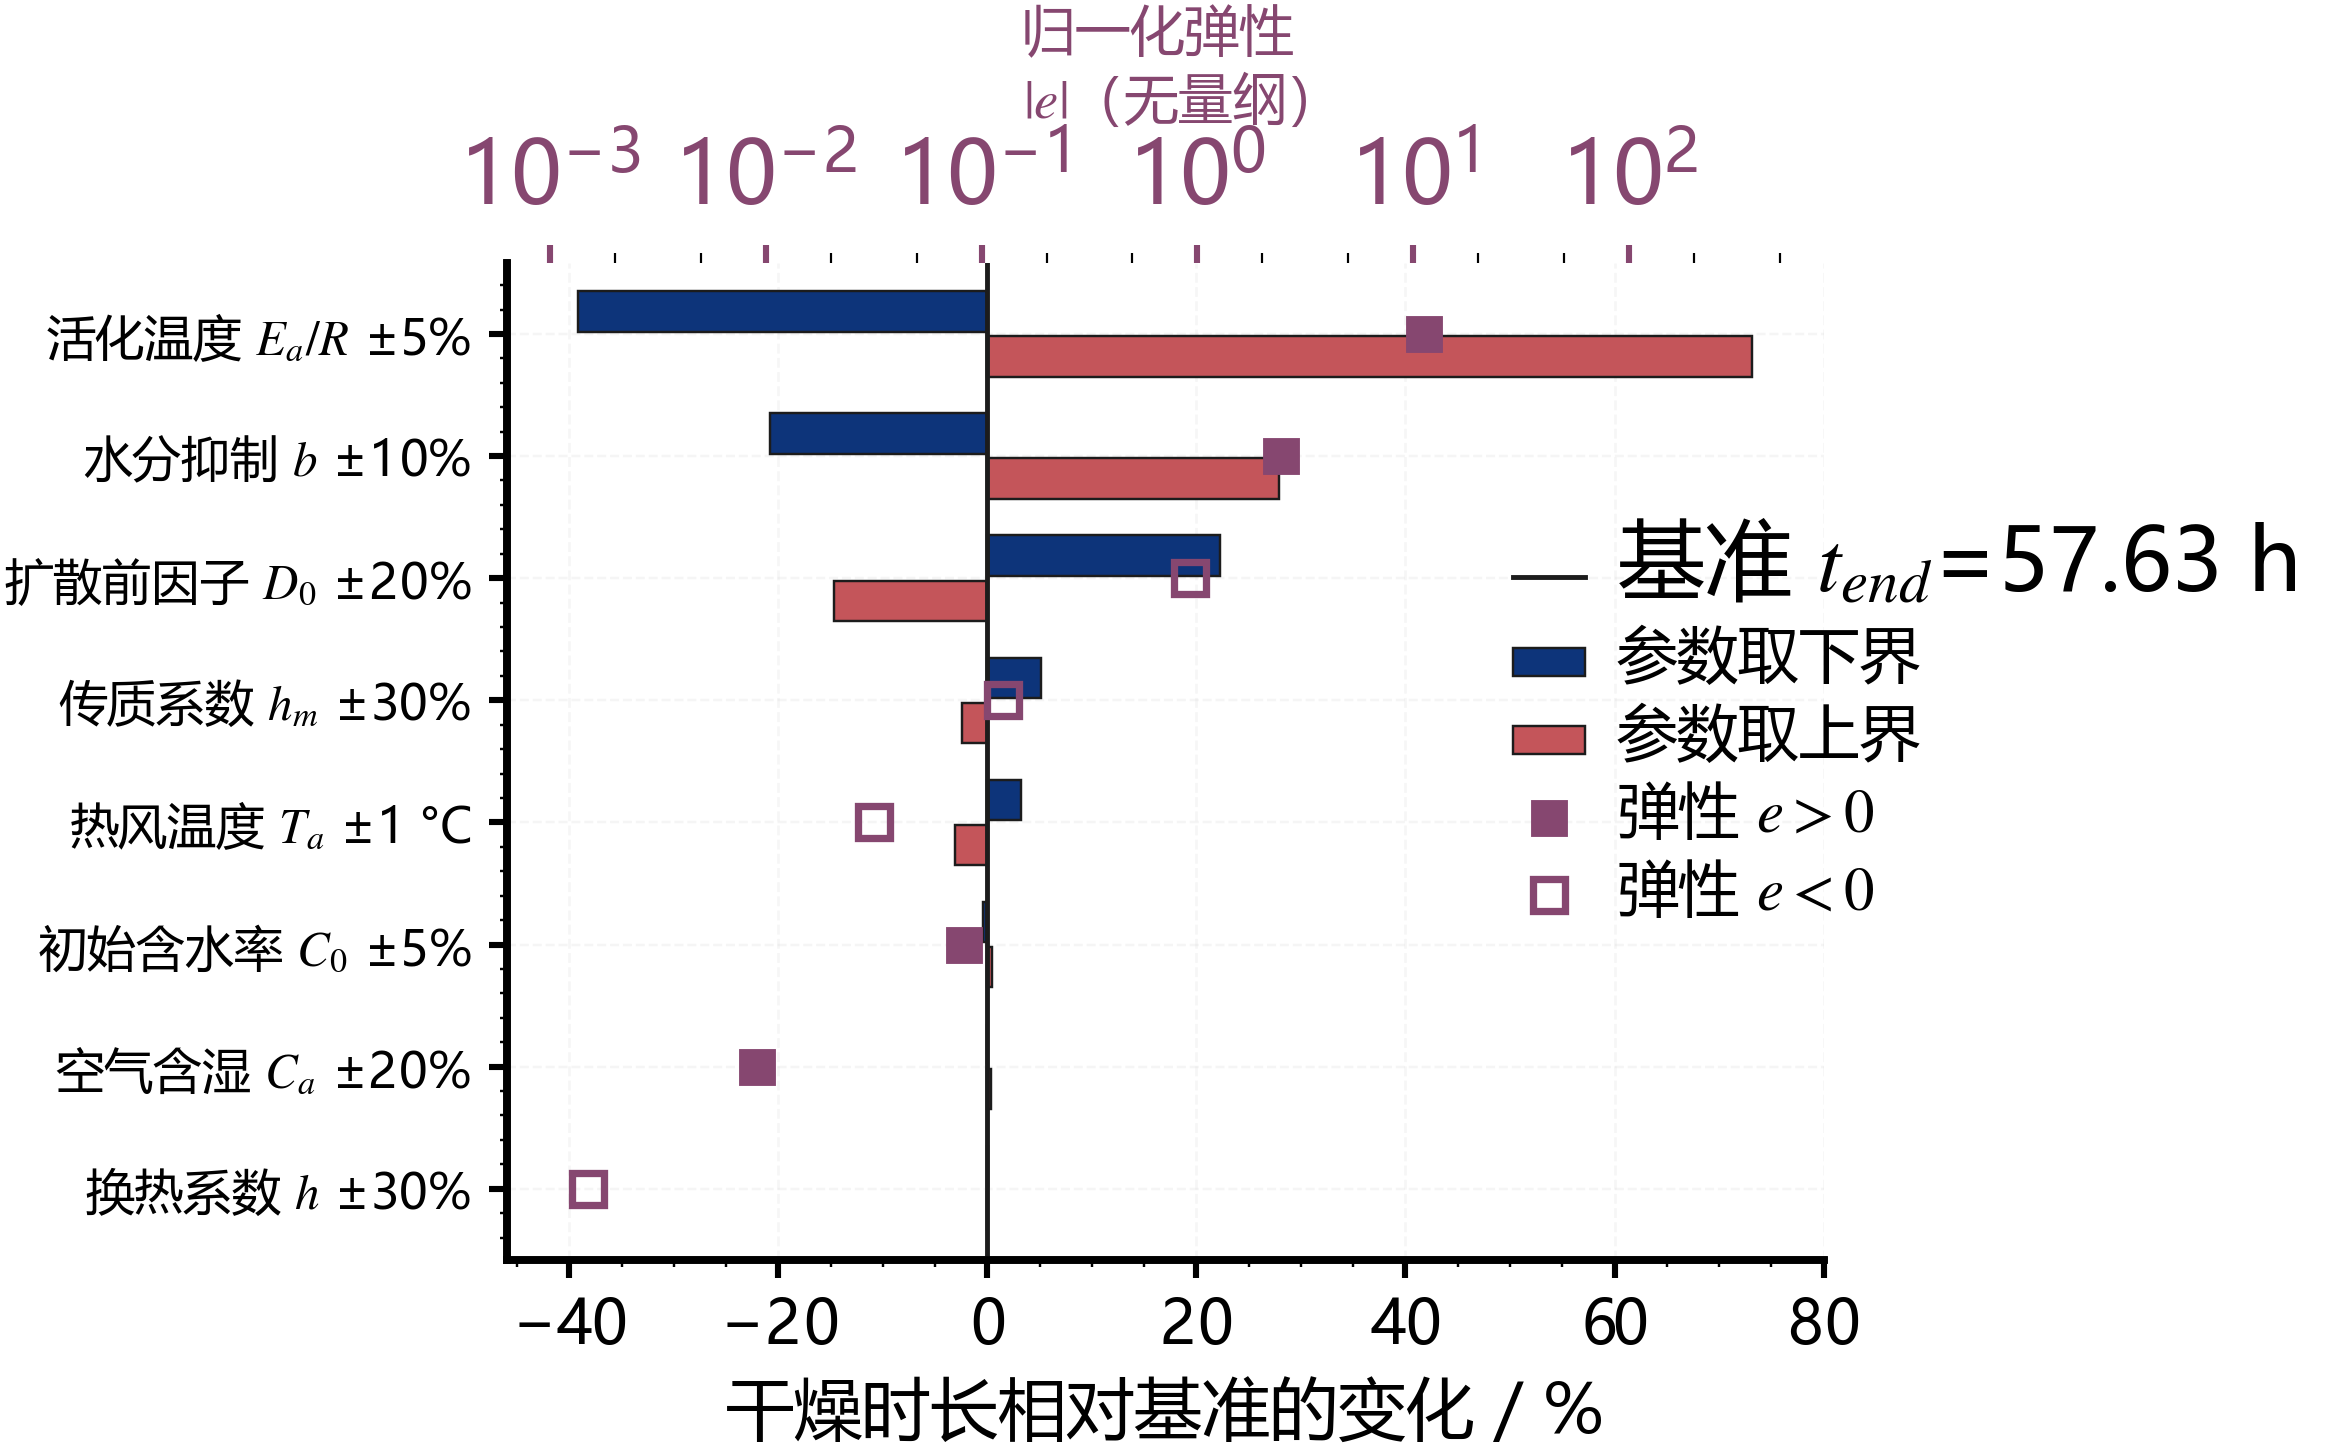
\includegraphics[width=0.94\textwidth]{figures/fig_q3_sensitivity_tornado.png}
  \caption[问题三八参数龙卷风敏感度]{问题三八参数龙卷风敏感度图：左半为各参数双向扰动引起的 $t_{end}$ 变化，右轴散点为归一化弹性。基准 $t_{end}$=57.625\,h。Arrhenius 活化温度 3850 K 的 $\pm5\%$ 扰动即产生 35.061--99.777\,h 的跨度（$-39.2\%/+73.1\%$），弹性 11.23，居首位；其 Spearman 秩相关 0.868 亦为八参数最高，两种排序一致。}
  \label{fig:q3_sensitivity_tornado}
\end{figure}

\begin{figure}[H]
  \centering
  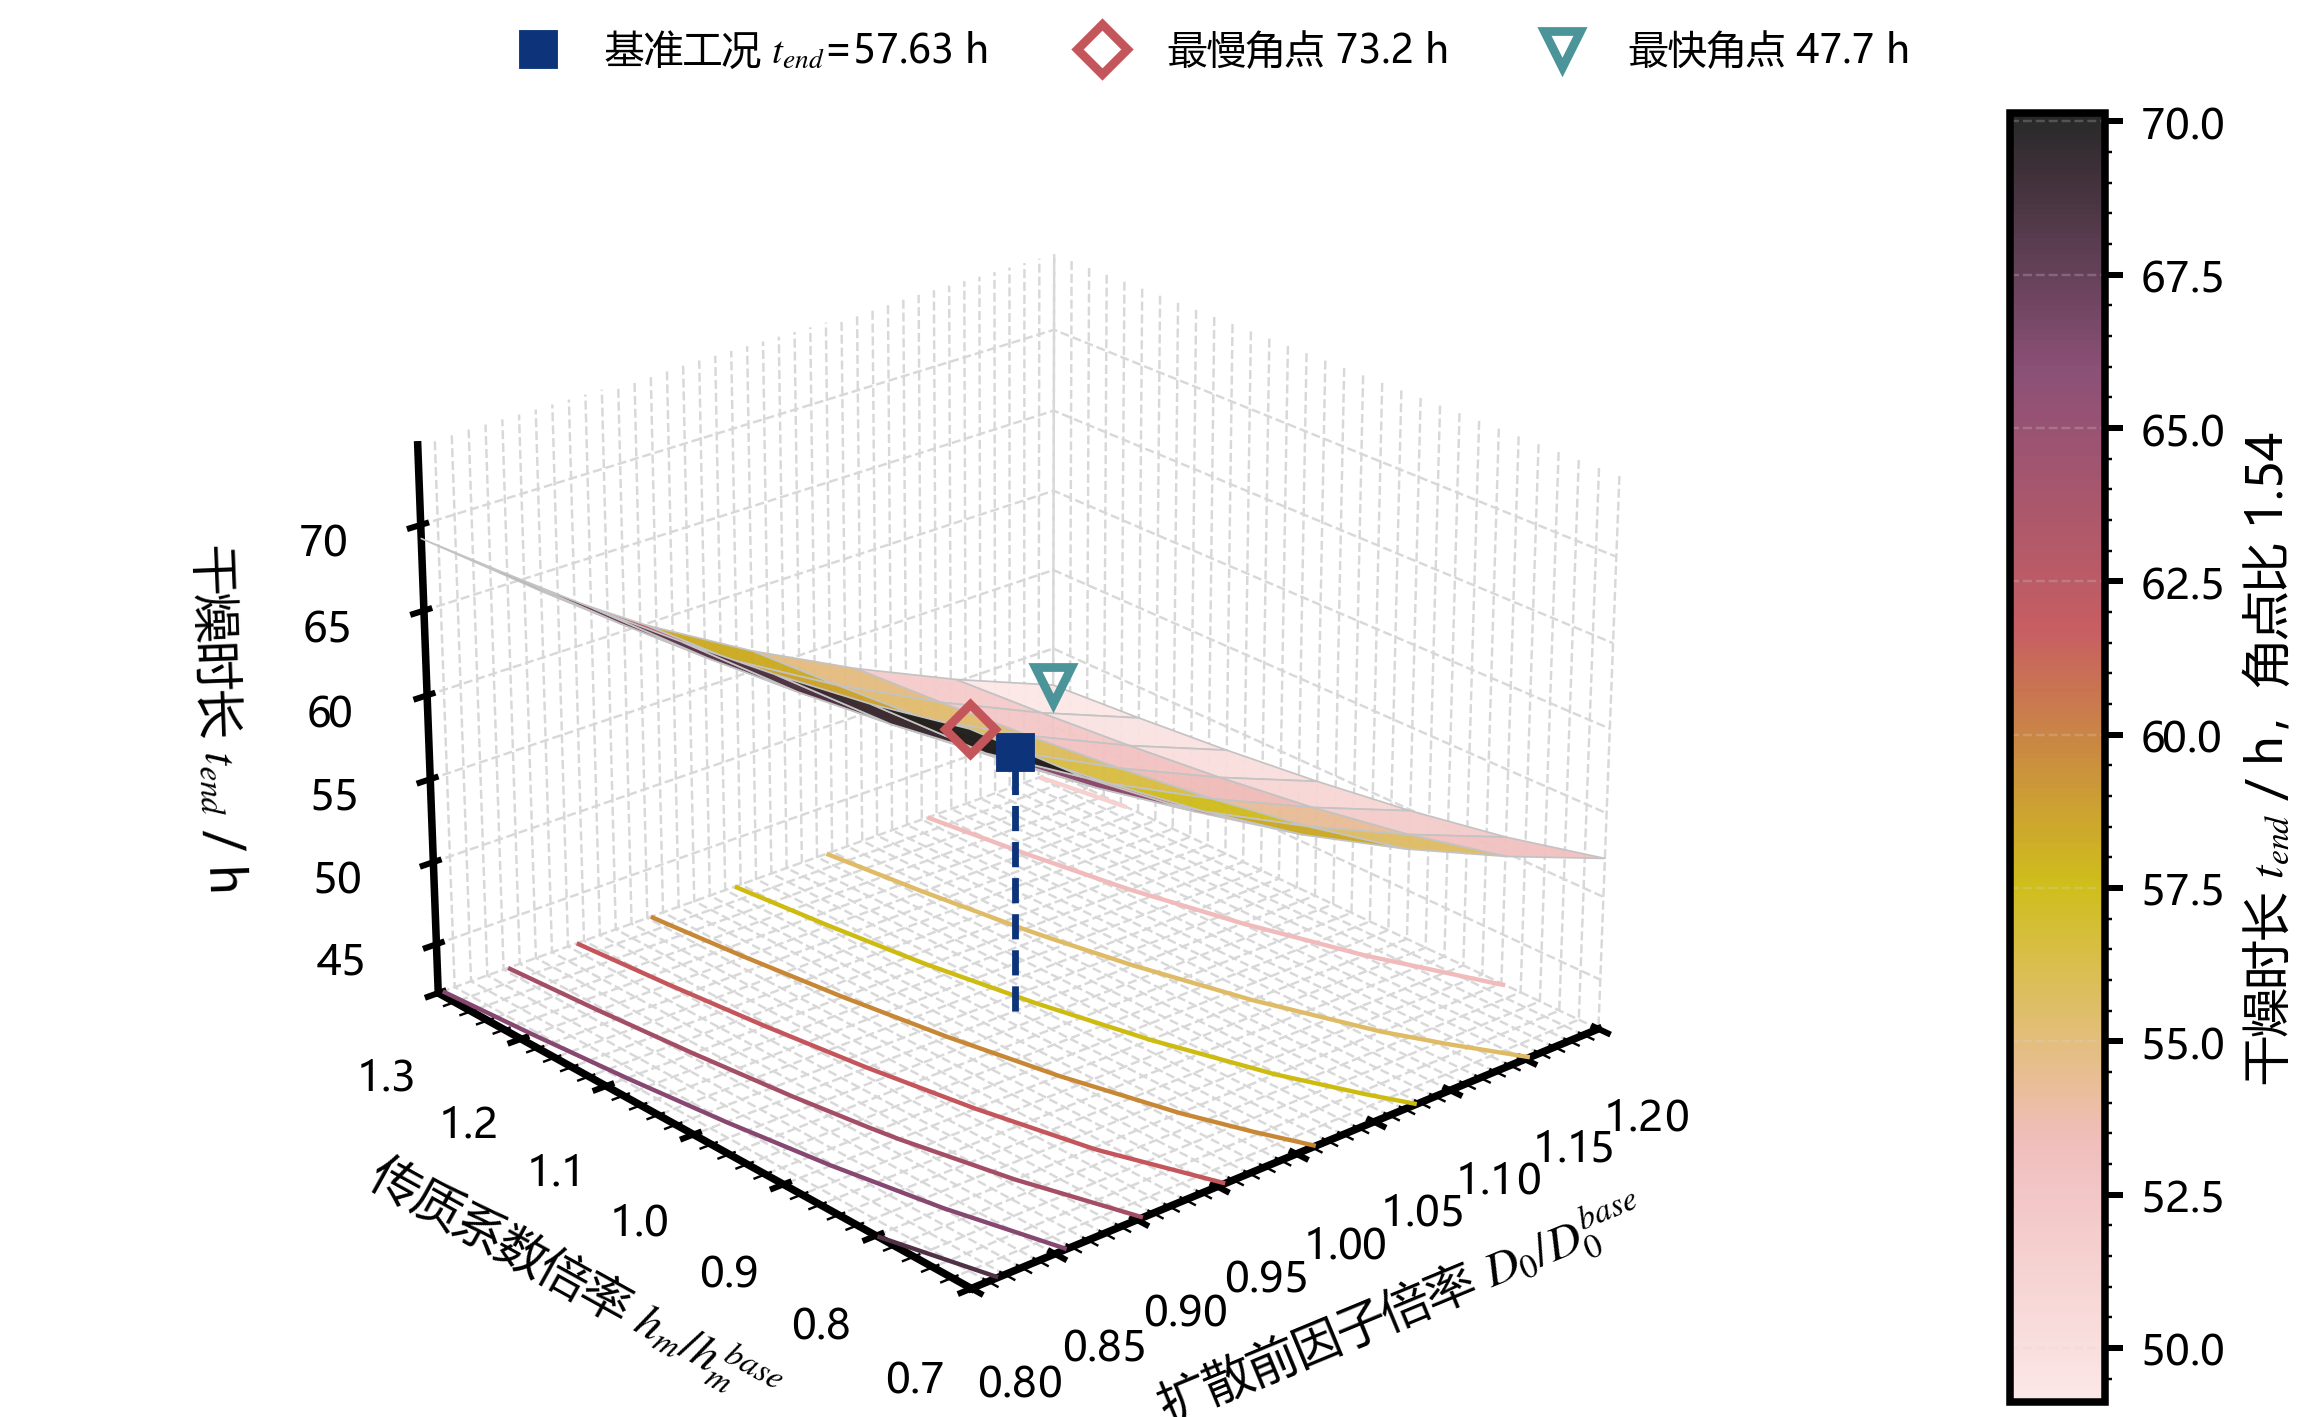
\includegraphics[width=0.92\textwidth]{figures/fig_q3_sensitivity_surface.png}
  \caption[$(h_m, D_0)$ 双因子响应面]{对流传质系数 $h_m$ 与扩散前因子 $D_0$ 双因子对 $t_{end}$ 的三维响应面，底面为等值线投影。两因子各取 7 档倍率（$D_0$：0.80--1.20，$h_m$：0.70--1.30），共 49 次真实求解；最慢角点 73.16\,h、最快角点 47.65\,h、基准 57.63\,h，角点比 1.535。曲面沿 $D_0$ 与 $h_m$ 两个方向均单调，无鞍点或折叠。}
  \label{fig:q3_sensitivity_surface}
\end{figure}

\begin{figure}[H]
  \centering
  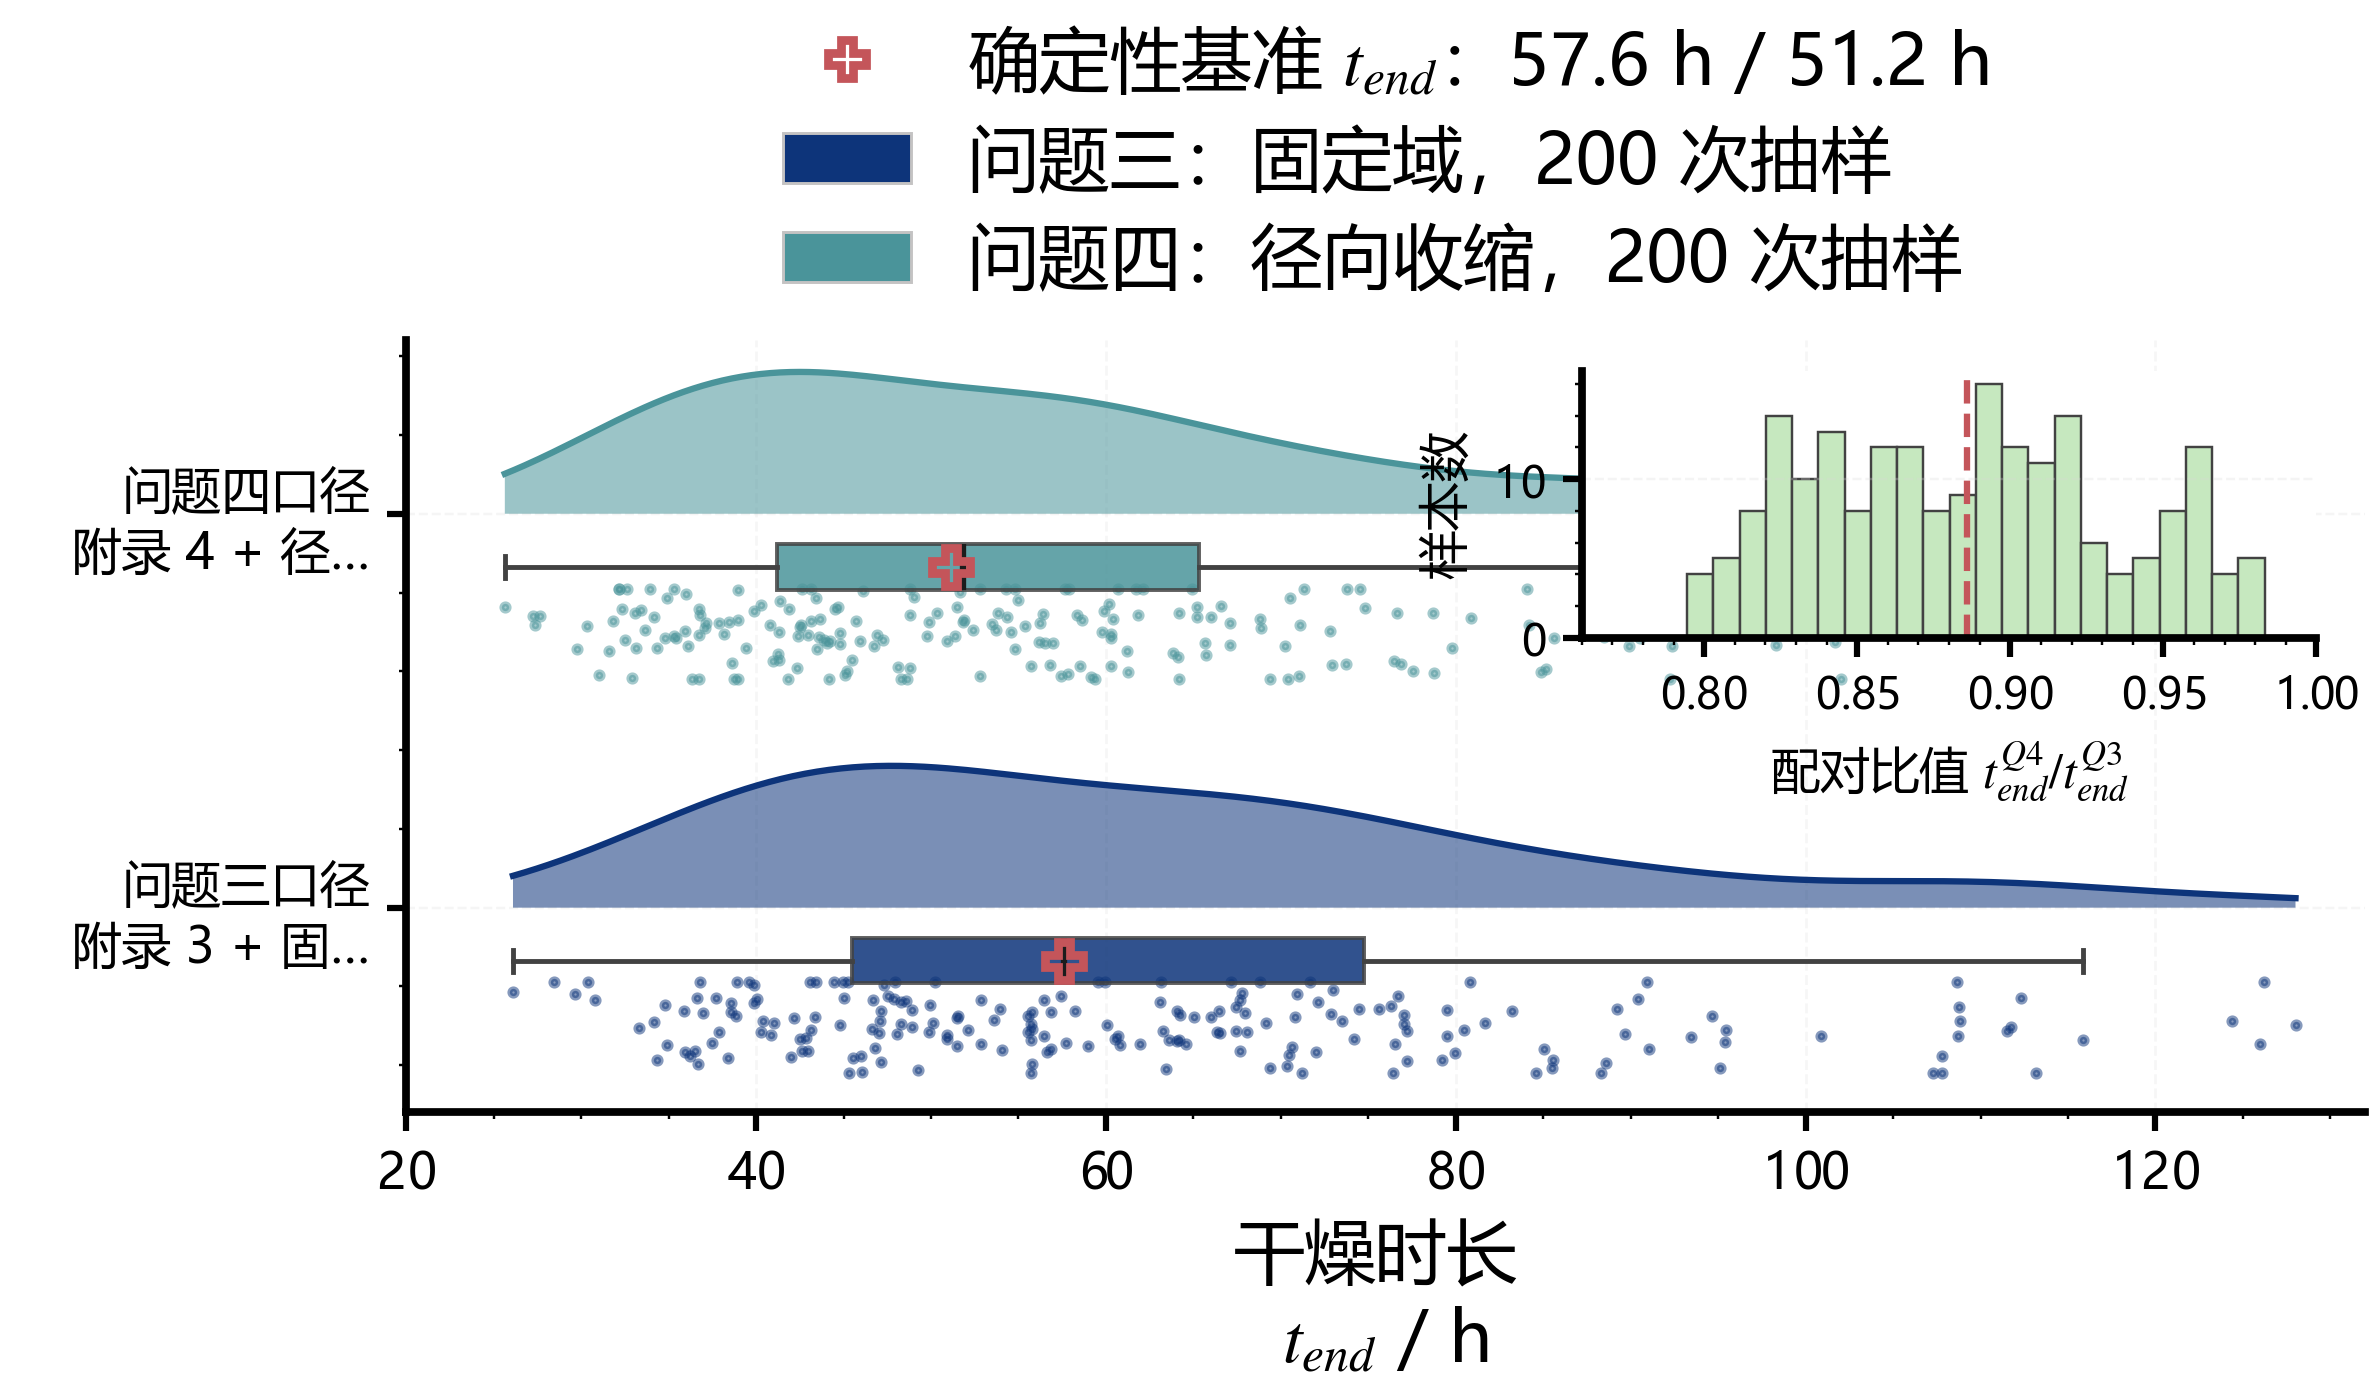
\includegraphics[width=0.94\textwidth]{figures/fig_q34_robustness.png}
  \caption[问题三/四干燥时长配对雨云图]{同一 200 组 LHS 矩阵驱动下两种口径干燥时长的雨云图（半小提琴 + 箱线 + 抖动散点）。下行问题三口径（附录 3 + 固定域）：$t_{end}$ 中位数 57.588\,h、90\% 区间 35.845--108.744\,h、变异系数 0.358；上行问题四口径（附录 4 + 径向收缩）：中位数 51.847\,h、90\% 区间 32.191--91.574\,h、变异系数 0.334。插图为逐样本配对比值的分布：收缩口径 100\% 短于固定口径，比值中位数 0.886、范围 0.794--0.983，故\emph{收缩加快干燥}不依赖单组参数取值。}
  \label{fig:q34_robustness}
\end{figure}

\begin{figure}[H]
  \centering
  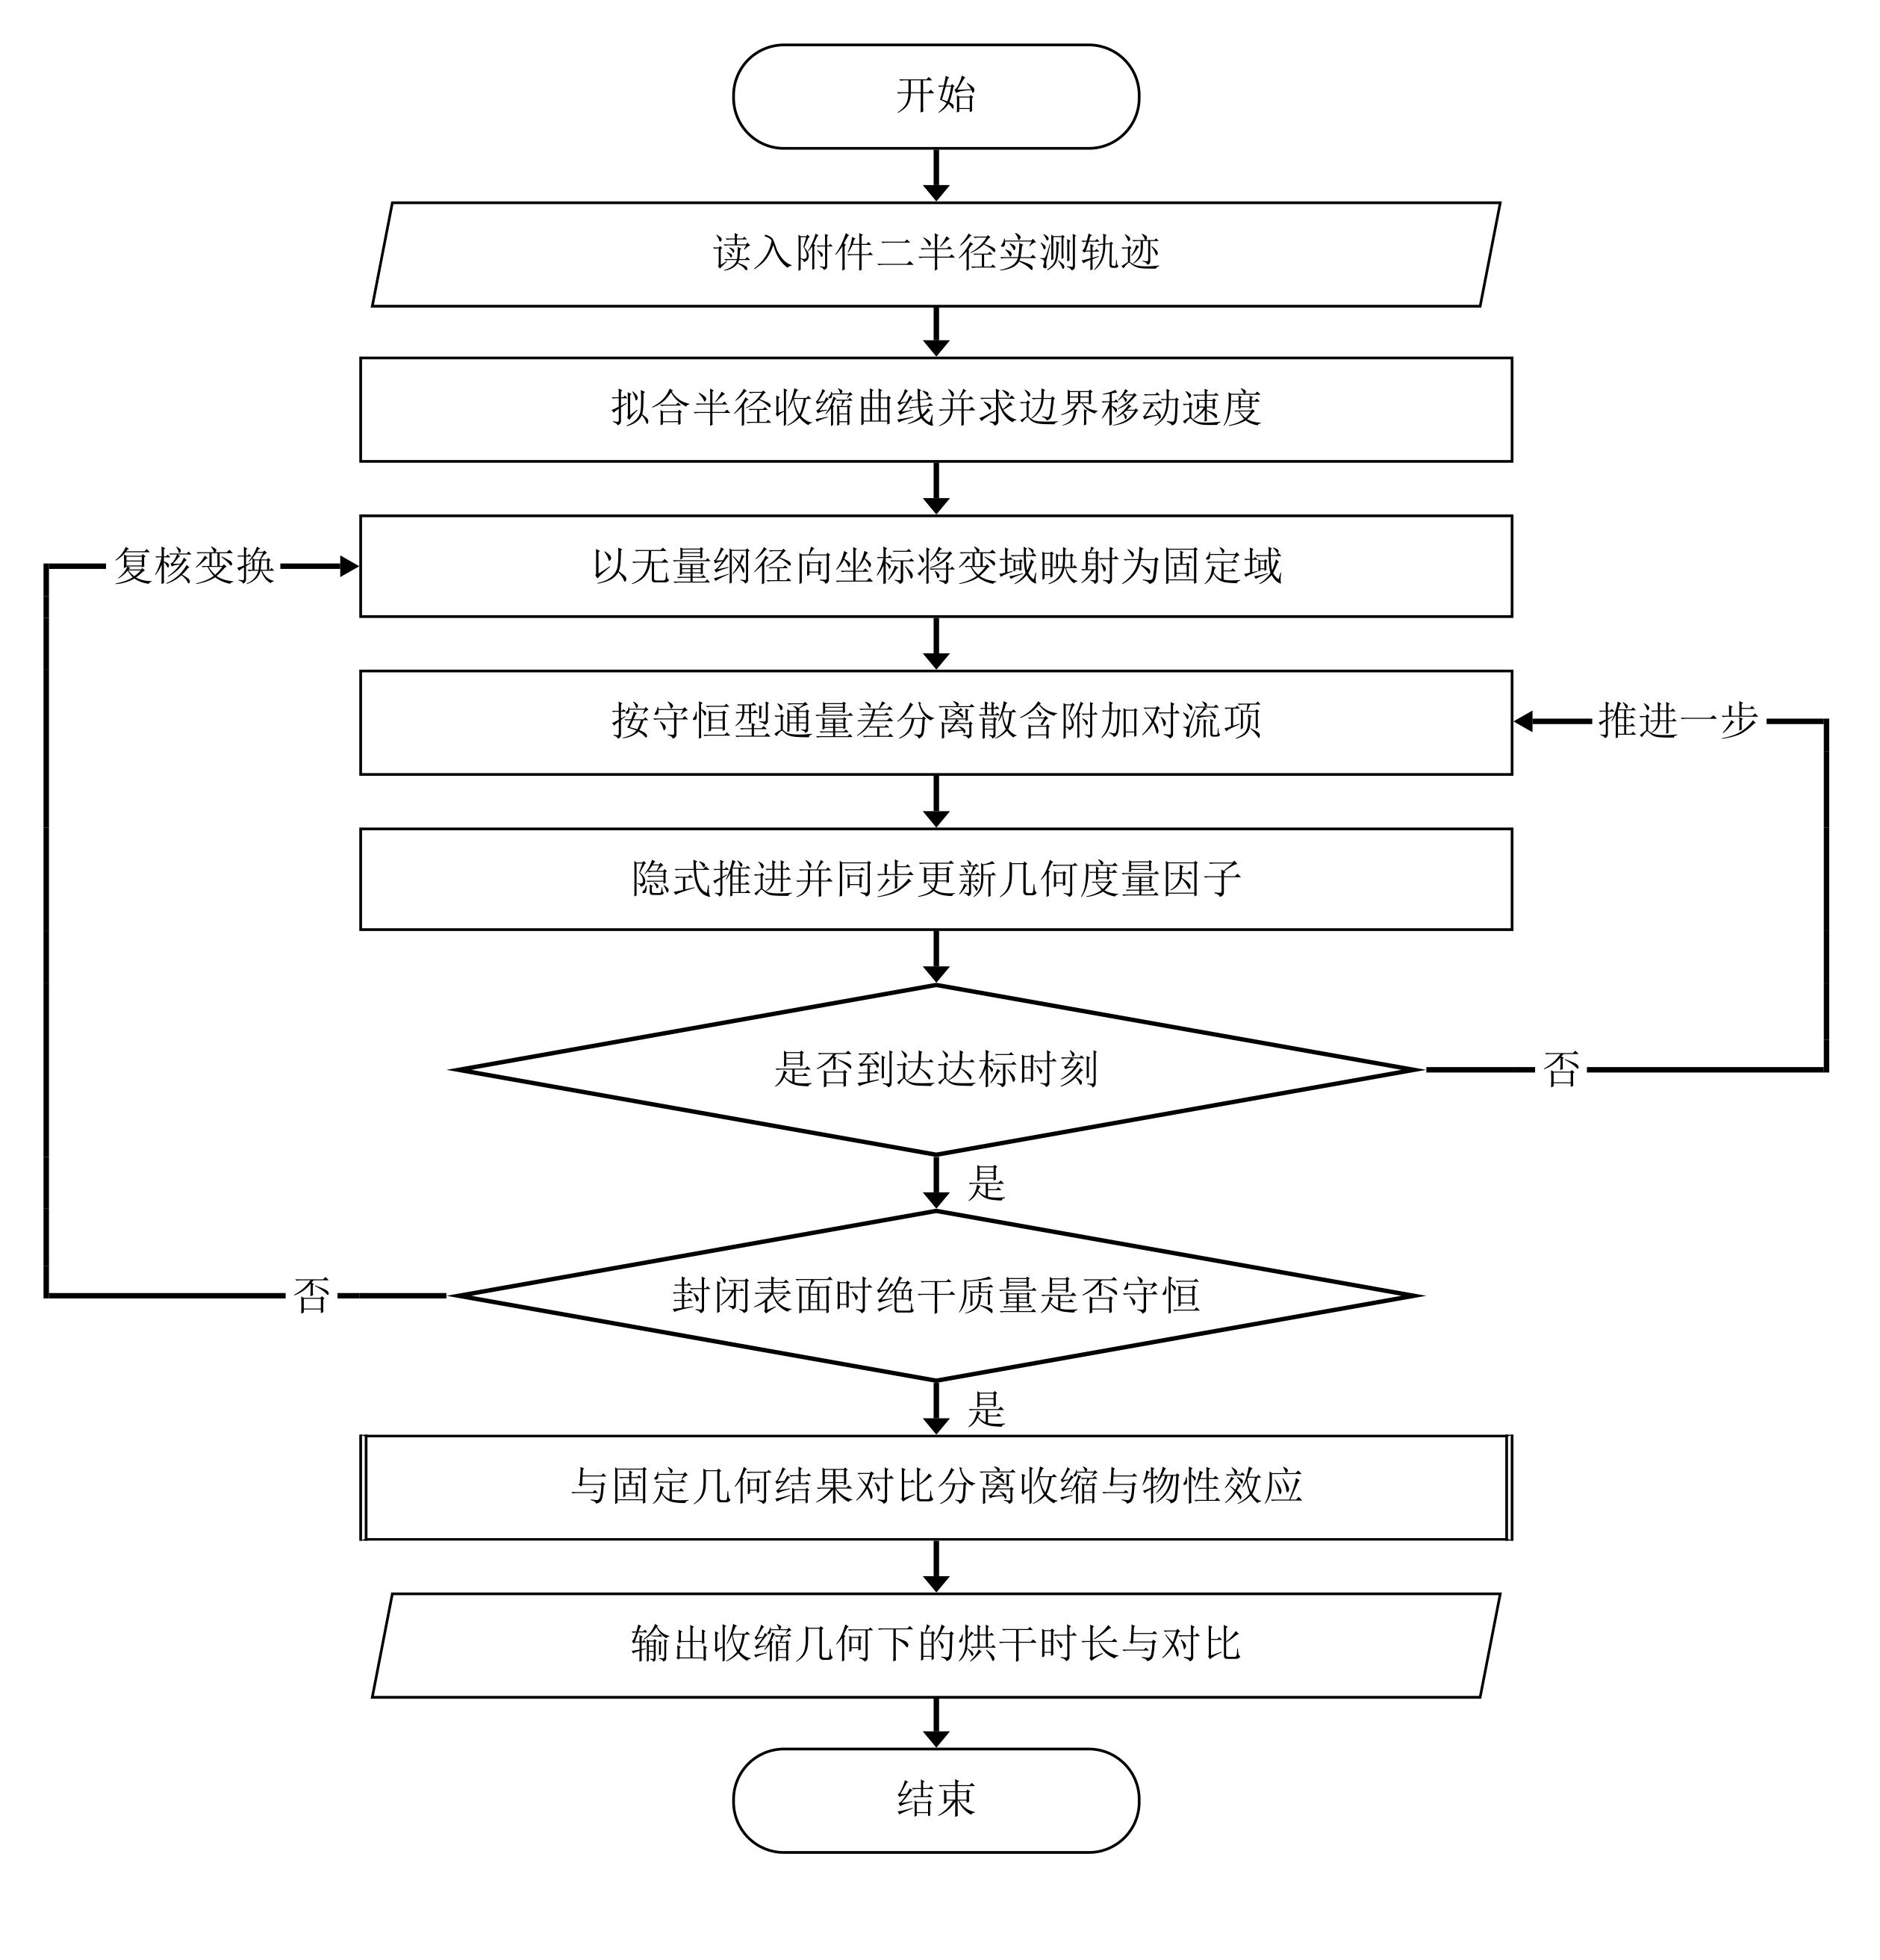
\includegraphics[width=0.95\textwidth]{figures/fig_flow_q4.png}
  \caption[问题四求解流程]{问题四求解流程。在问题三基础上引入附件 2 的半径轨迹 $R(t)$，经无量纲坐标 $\eta=r/R(t)$ 映射到固定计算域后仍用同一套离散，代价是方程多出一个几何放大因子与一项由动边界产生的对流项；干基质量守恒作为独立校核，不满足即回到收缩速率的标定。末端与问题三同判据对照，得到收缩对烘干时长的净影响。}
  \label{fig:flow_q4}
\end{figure}

\begin{figure}[H]
  \centering
  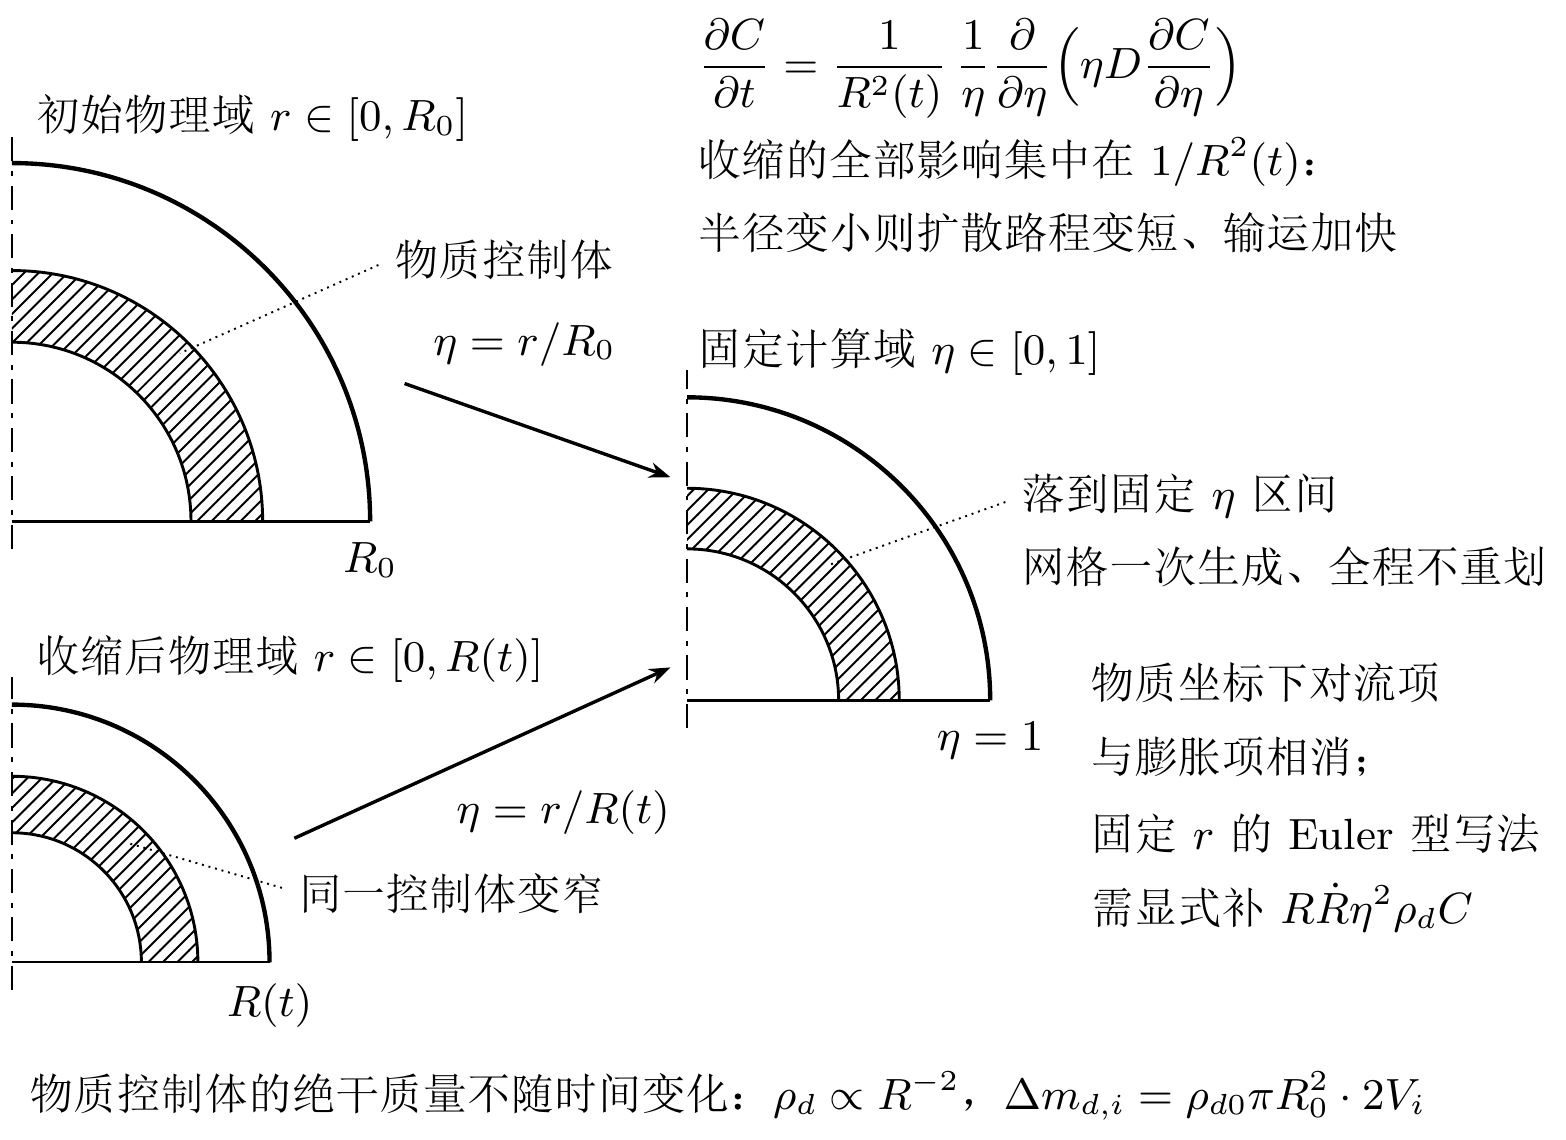
\includegraphics[width=1.00\textwidth]{figures/tikz_q4_moving_boundary.png}
  \caption[收缩域到固定域的坐标变换]{收缩域到固定计算域的坐标变换。左侧物理域半径随时间由 2.00\,cm 收缩到 1.20\,cm，网格若随边界移动则每步都要重新生成；经 $\eta=r/R(t)$ 映射后计算域恒为 $\eta\in[0,1]$，网格一次生成、全程复用。代价写在右侧：方程多出几何放大因子 $1/R^{2}(t)$，且物质坐标下的 Euler 型写法需显式补入由边界运动产生的对流项。干基密度按 $\rho_d\propto R^{-2}$ 同步更新，使收缩不虚增或虚减干物质。}
  \label{fig:tikz_q4_moving_boundary}
\end{figure}

\begin{figure}[H]
  \centering
  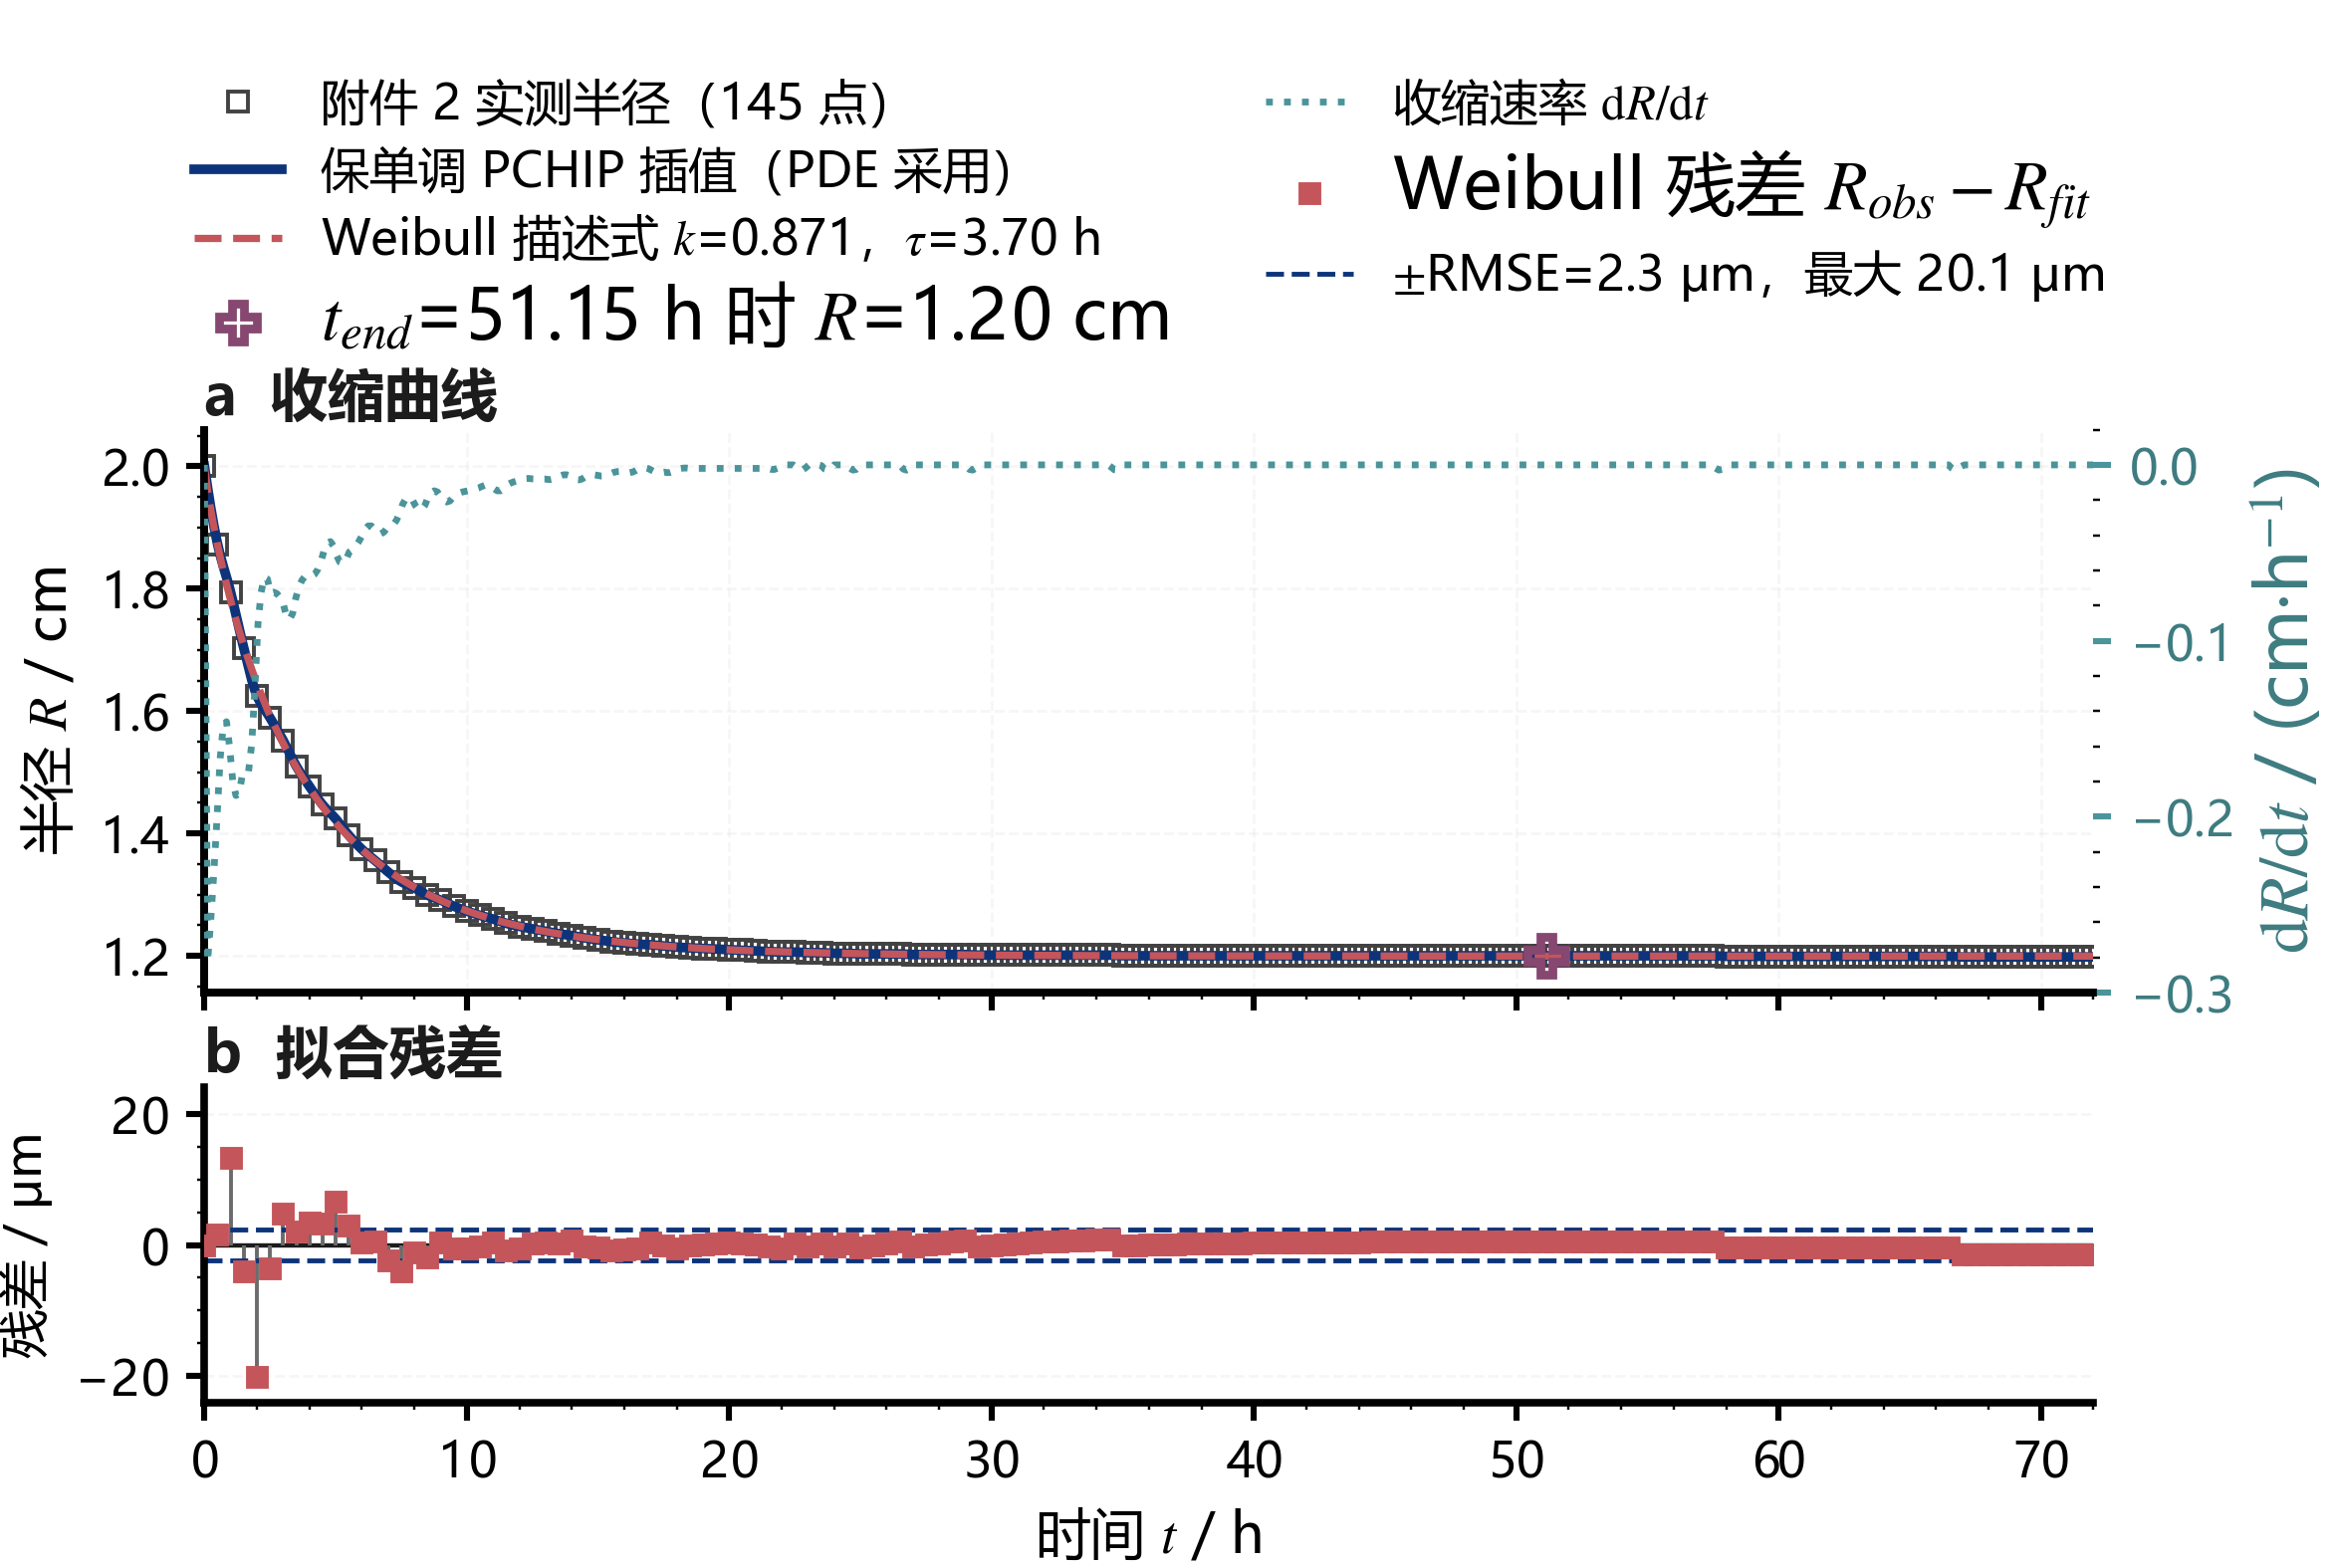
\includegraphics[width=0.94\textwidth]{figures/fig_q4_radius_fit.png}
  \caption[附件 2 半径轨迹与收缩模型]{附件 2 半径实测轨迹与收缩模型。面板 a 叠合 145 个实测点、保单调 PCHIP 插值（PDE 实际采用）与 Weibull 描述式（$R_\infty$=1.1994\,cm，$\tau$=3.70\,h，$k$=0.8713），右轴为收缩速率 $\mathrm{d}R/\mathrm{d}t$；面板 b 为 Weibull 残差。半径自 2.00\,cm 单调降至 1.198\,cm（累计收缩 40.1\%），10000 点扫描下 $\mathrm{d}R/\mathrm{d}t\leq0$ 恒成立，最快收缩 $8.359\times10^{-5}$\,cm/s；插值复现实测点的最大绝对偏差 $2.2\times10^{-16}$\,cm。Weibull 仅作描述性参考（RMSE 23.3\,$\mu$m，最大 201.5\,$\mu$m），不进入 PDE 求解。}
  \label{fig:q4_radius_fit}
\end{figure}

\begin{figure}[H]
  \centering
  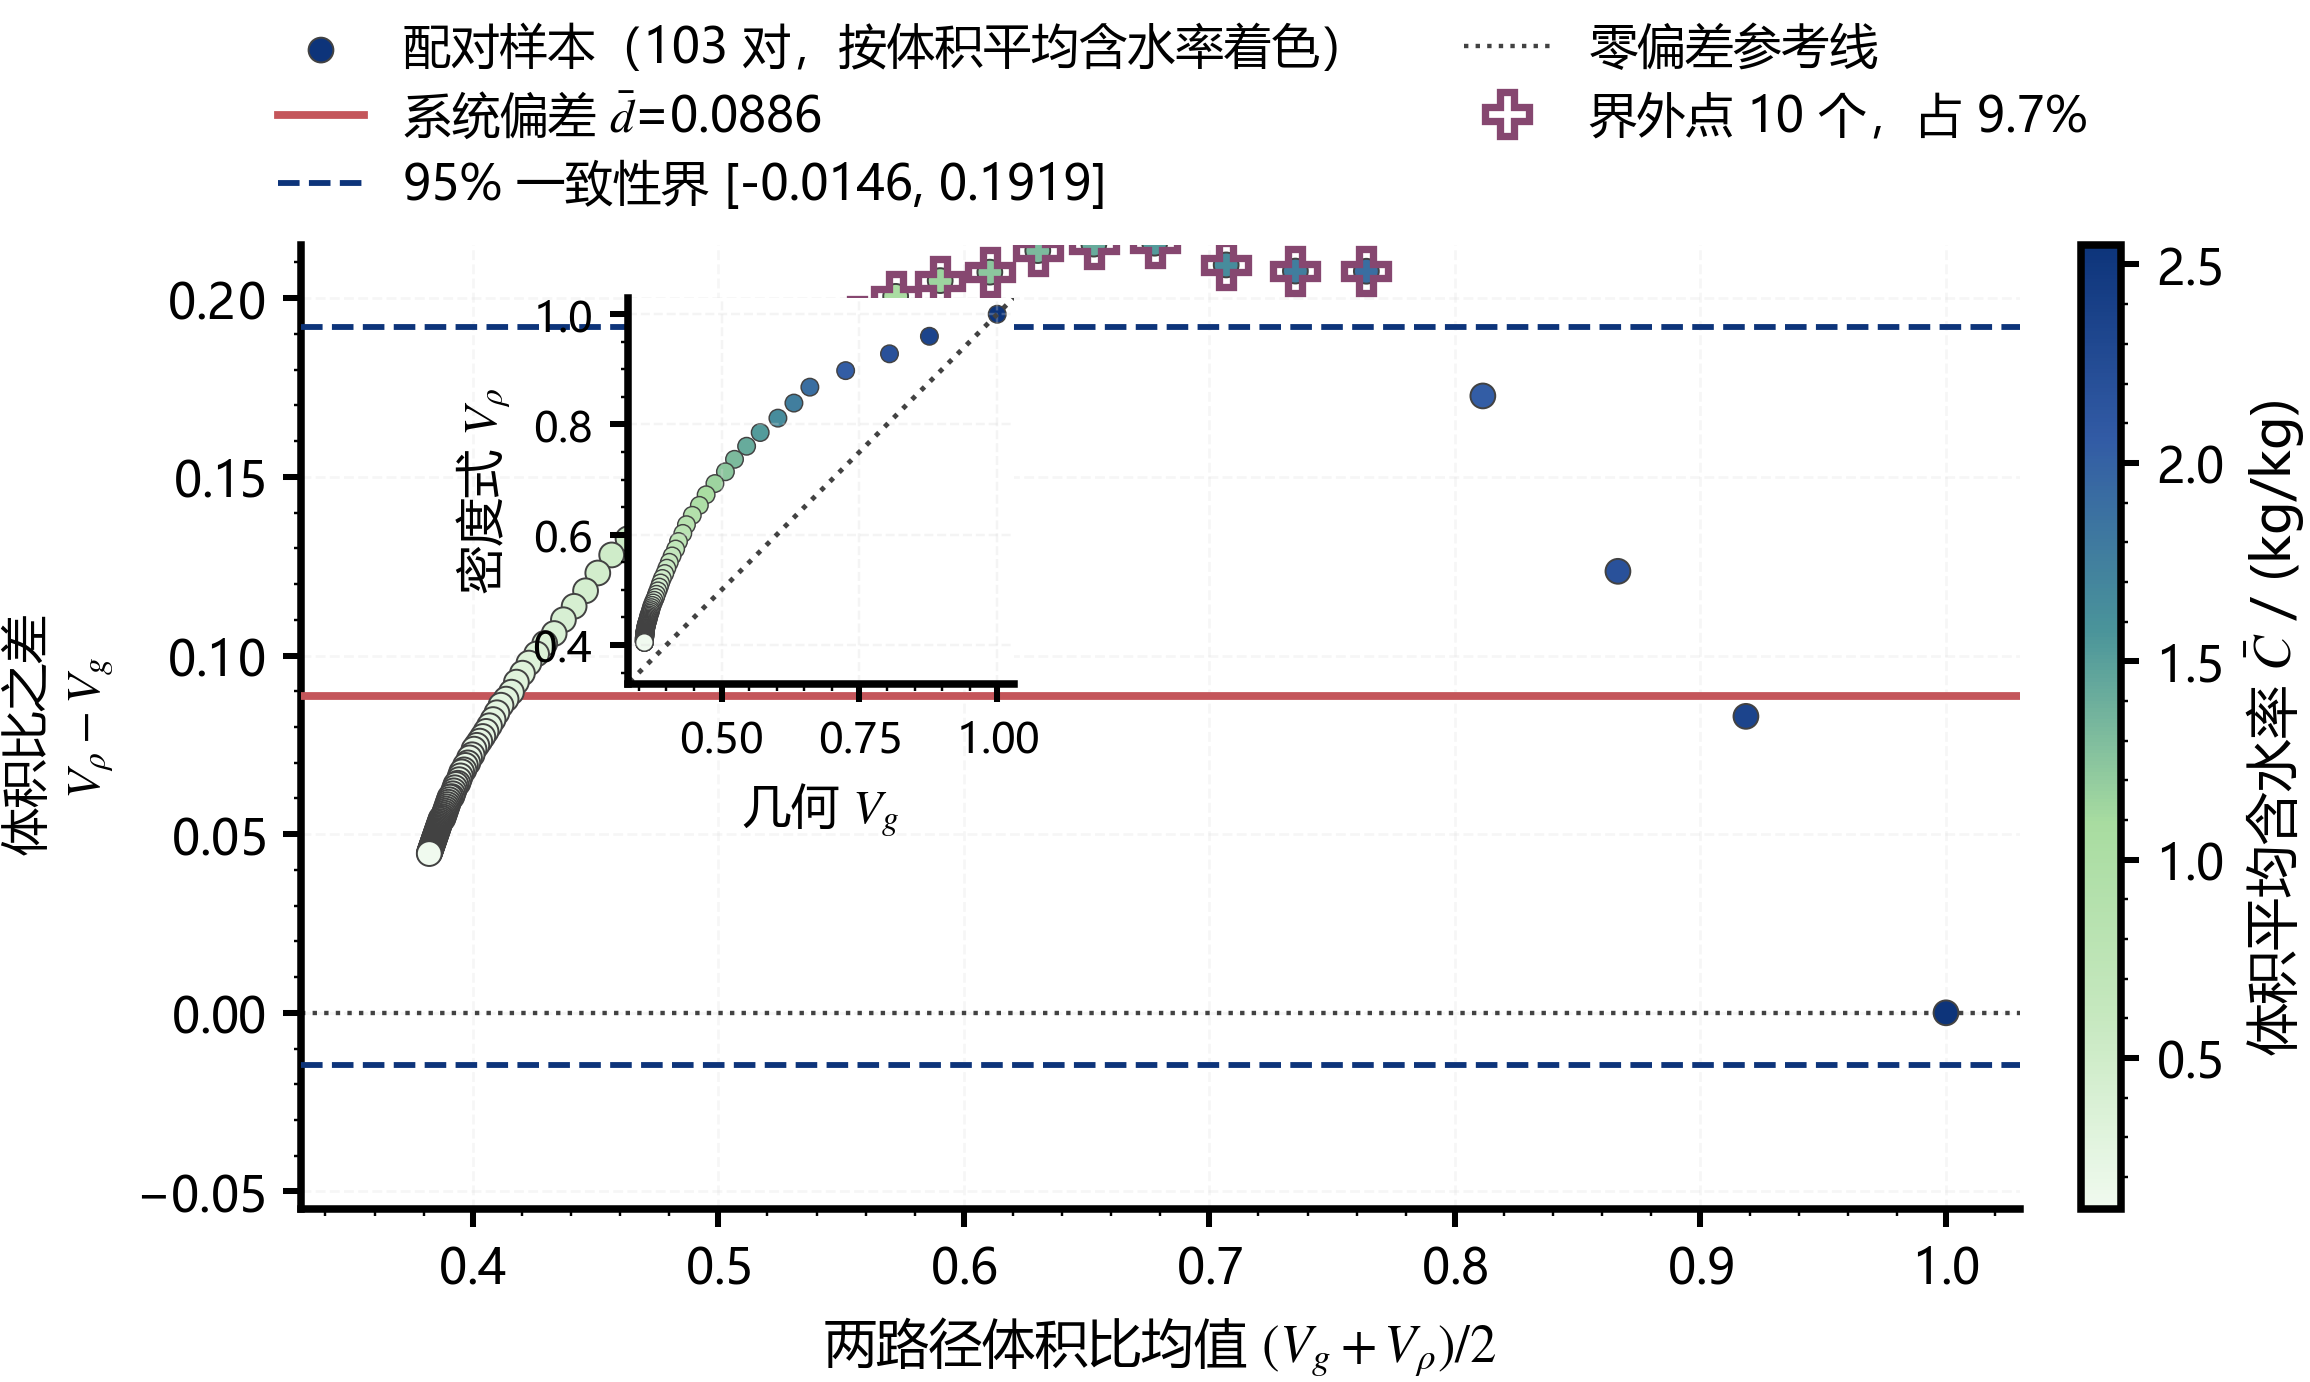
\includegraphics[width=0.92\textwidth]{figures/fig_q4_shrink_consistency.png}
  \caption[收缩量自洽性 Bland--Altman 检验]{几何体积比与密度式反推体积比的 Bland--Altman 一致性检验，散点按体积平均含水率着色，插图为两路径的直接对照（虚线为 $y=x$）。103 对样本的系统偏差 $\bar{d}$=0.0886，95\% 一致性界 [-0.0146, 0.1919]，界外 10 点（9.7\%）。终态两路径给出 0.3588 与 0.4144，相对差 13.42\%（判据 $<$20\%）：同阶但不完全自洽，故本文以附件 2 实测轨迹为准，未据密度式反向调参。}
  \label{fig:q4_shrink_consistency}
\end{figure}

\begin{figure}[H]
  \centering
  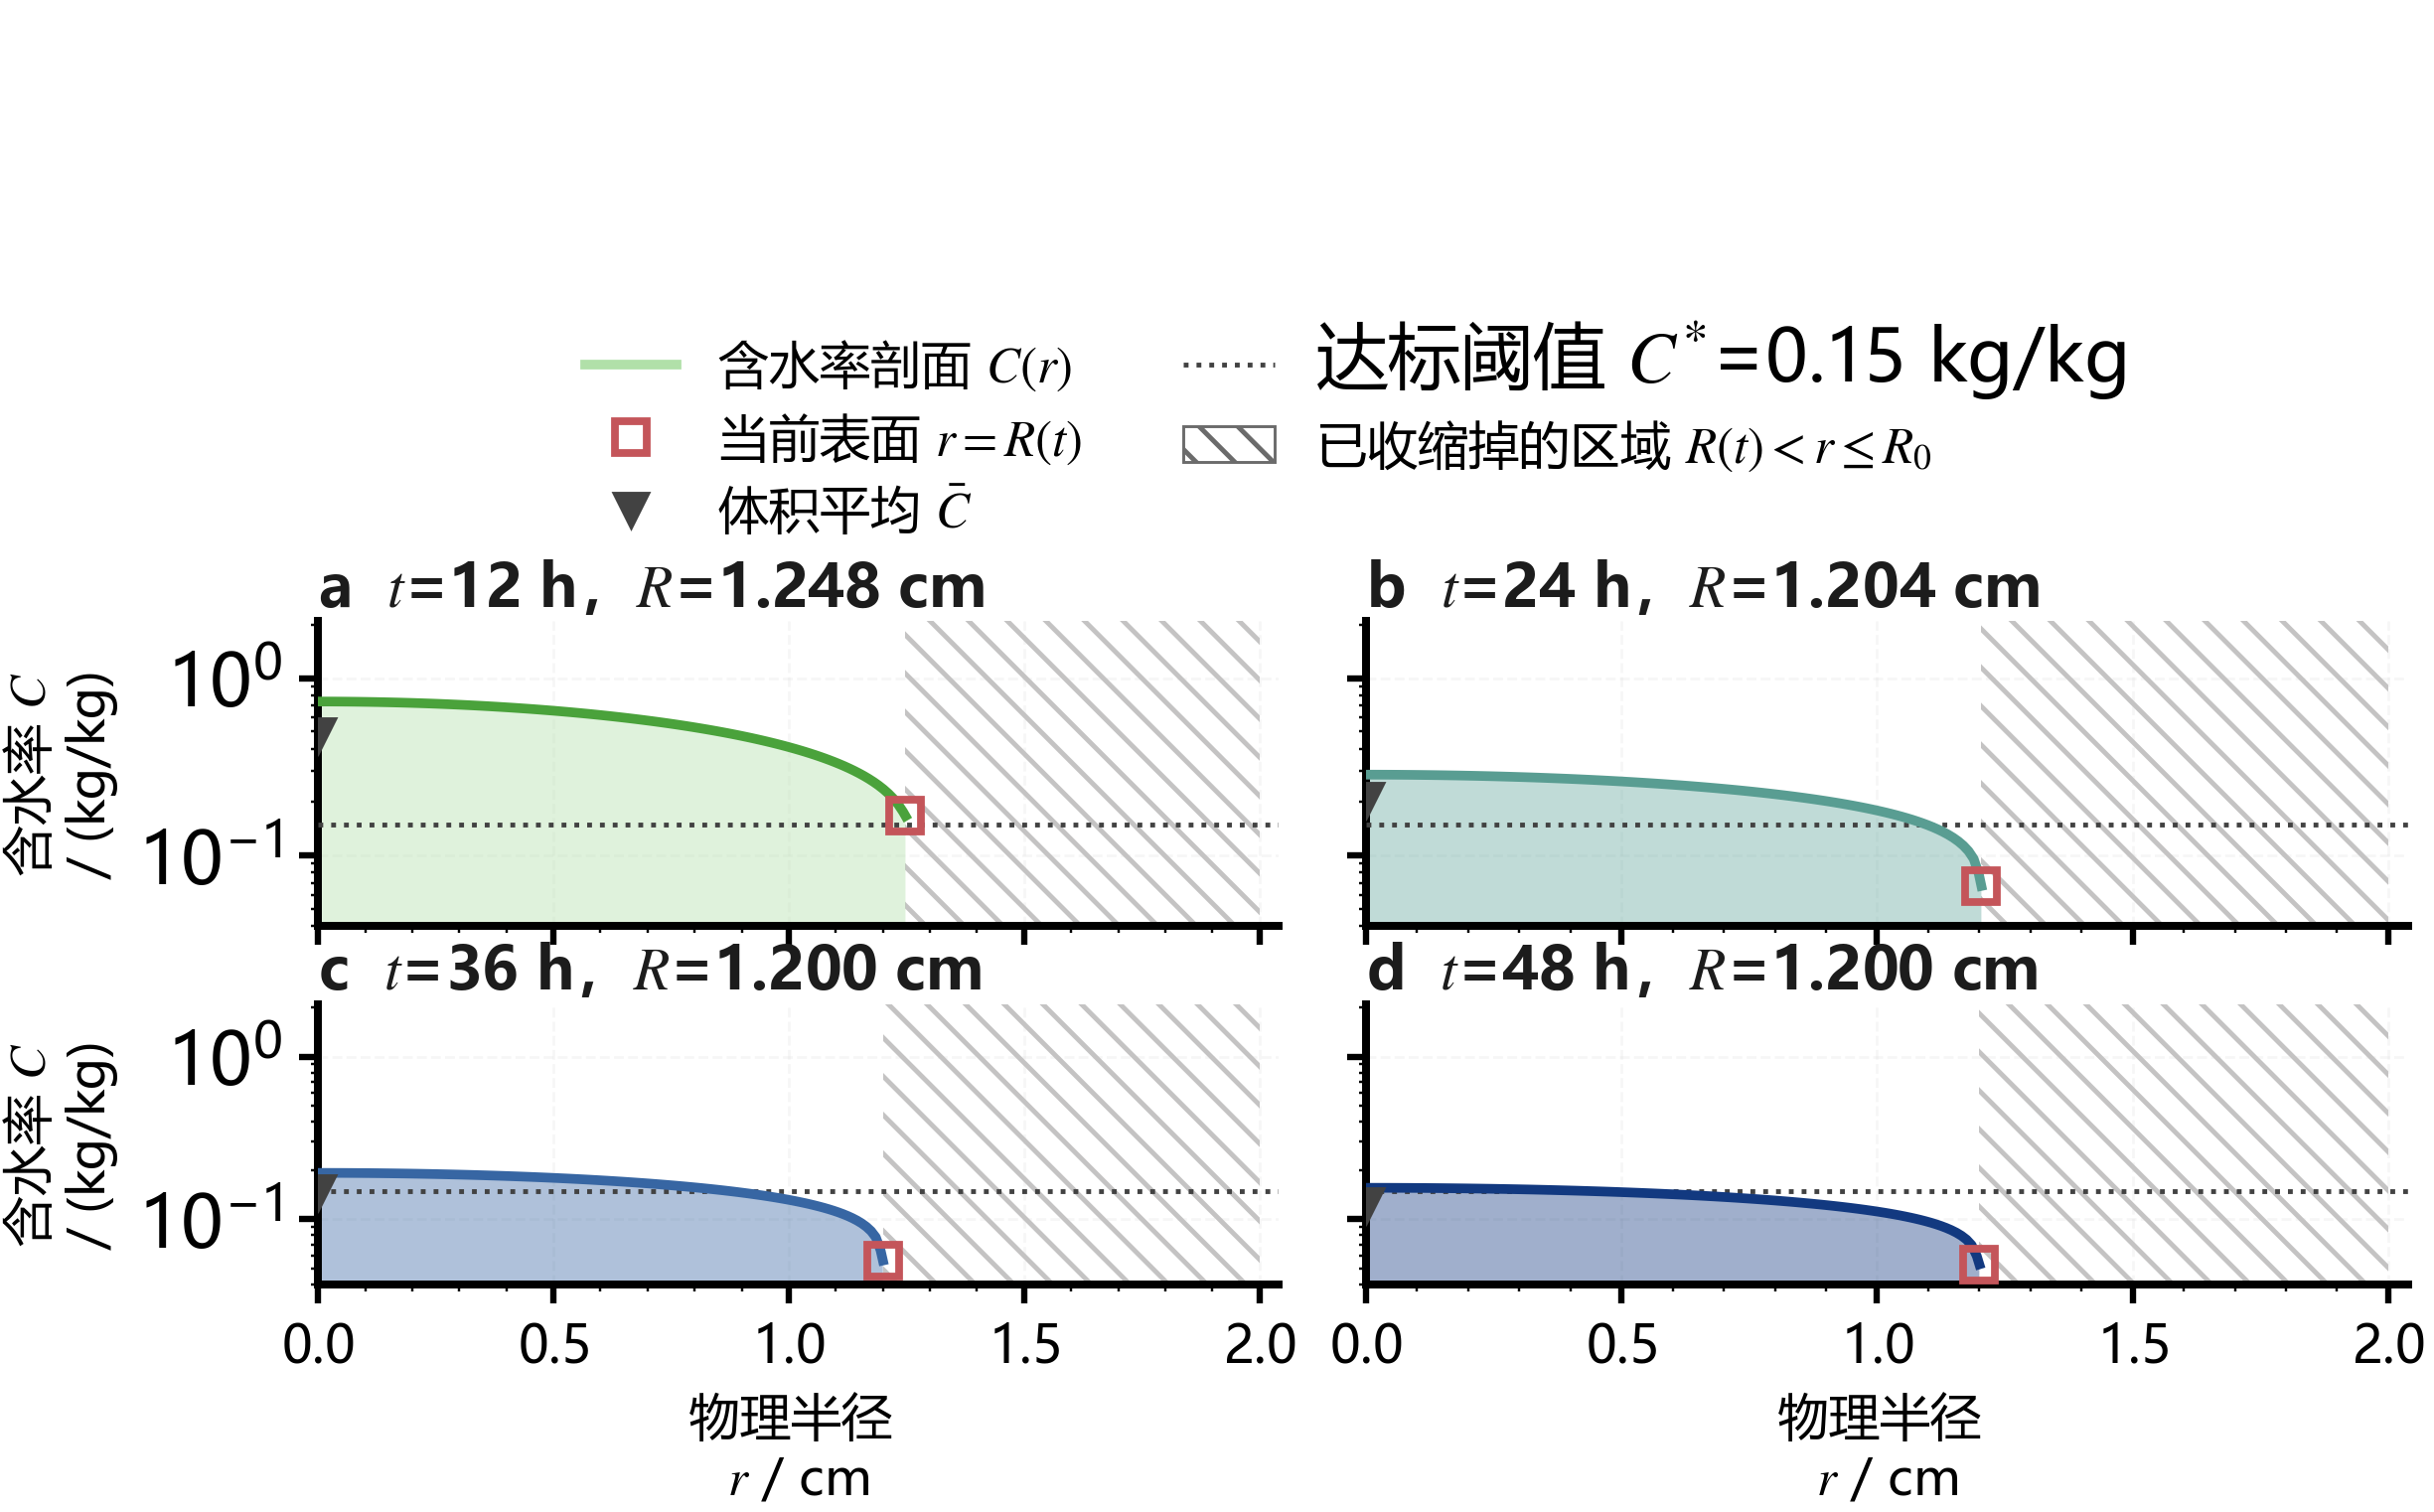
\includegraphics[width=0.96\textwidth]{figures/fig_q4_moving_boundary_frames.png}
  \caption[问题四真实几何含水率四帧]{问题四四帧真实几何下的含水率分布，横轴为物理半径，斜纹区为已收缩掉的 $R(t)<r\leq R_0$，纵轴取对数以同时容纳中心与表面两个量级。四帧 $t$=12/24/36/48\,h 对应 $R$=1.248/1.204/1.200/1.200\,cm。域在收缩的同时剖面整体下移，表面始终最先达标、中心最后达标；点线为 $C^{*}$=0.15\,kg/kg。}
  \label{fig:q4_moving_boundary_frames}
\end{figure}

\begin{figure}[H]
  \centering
  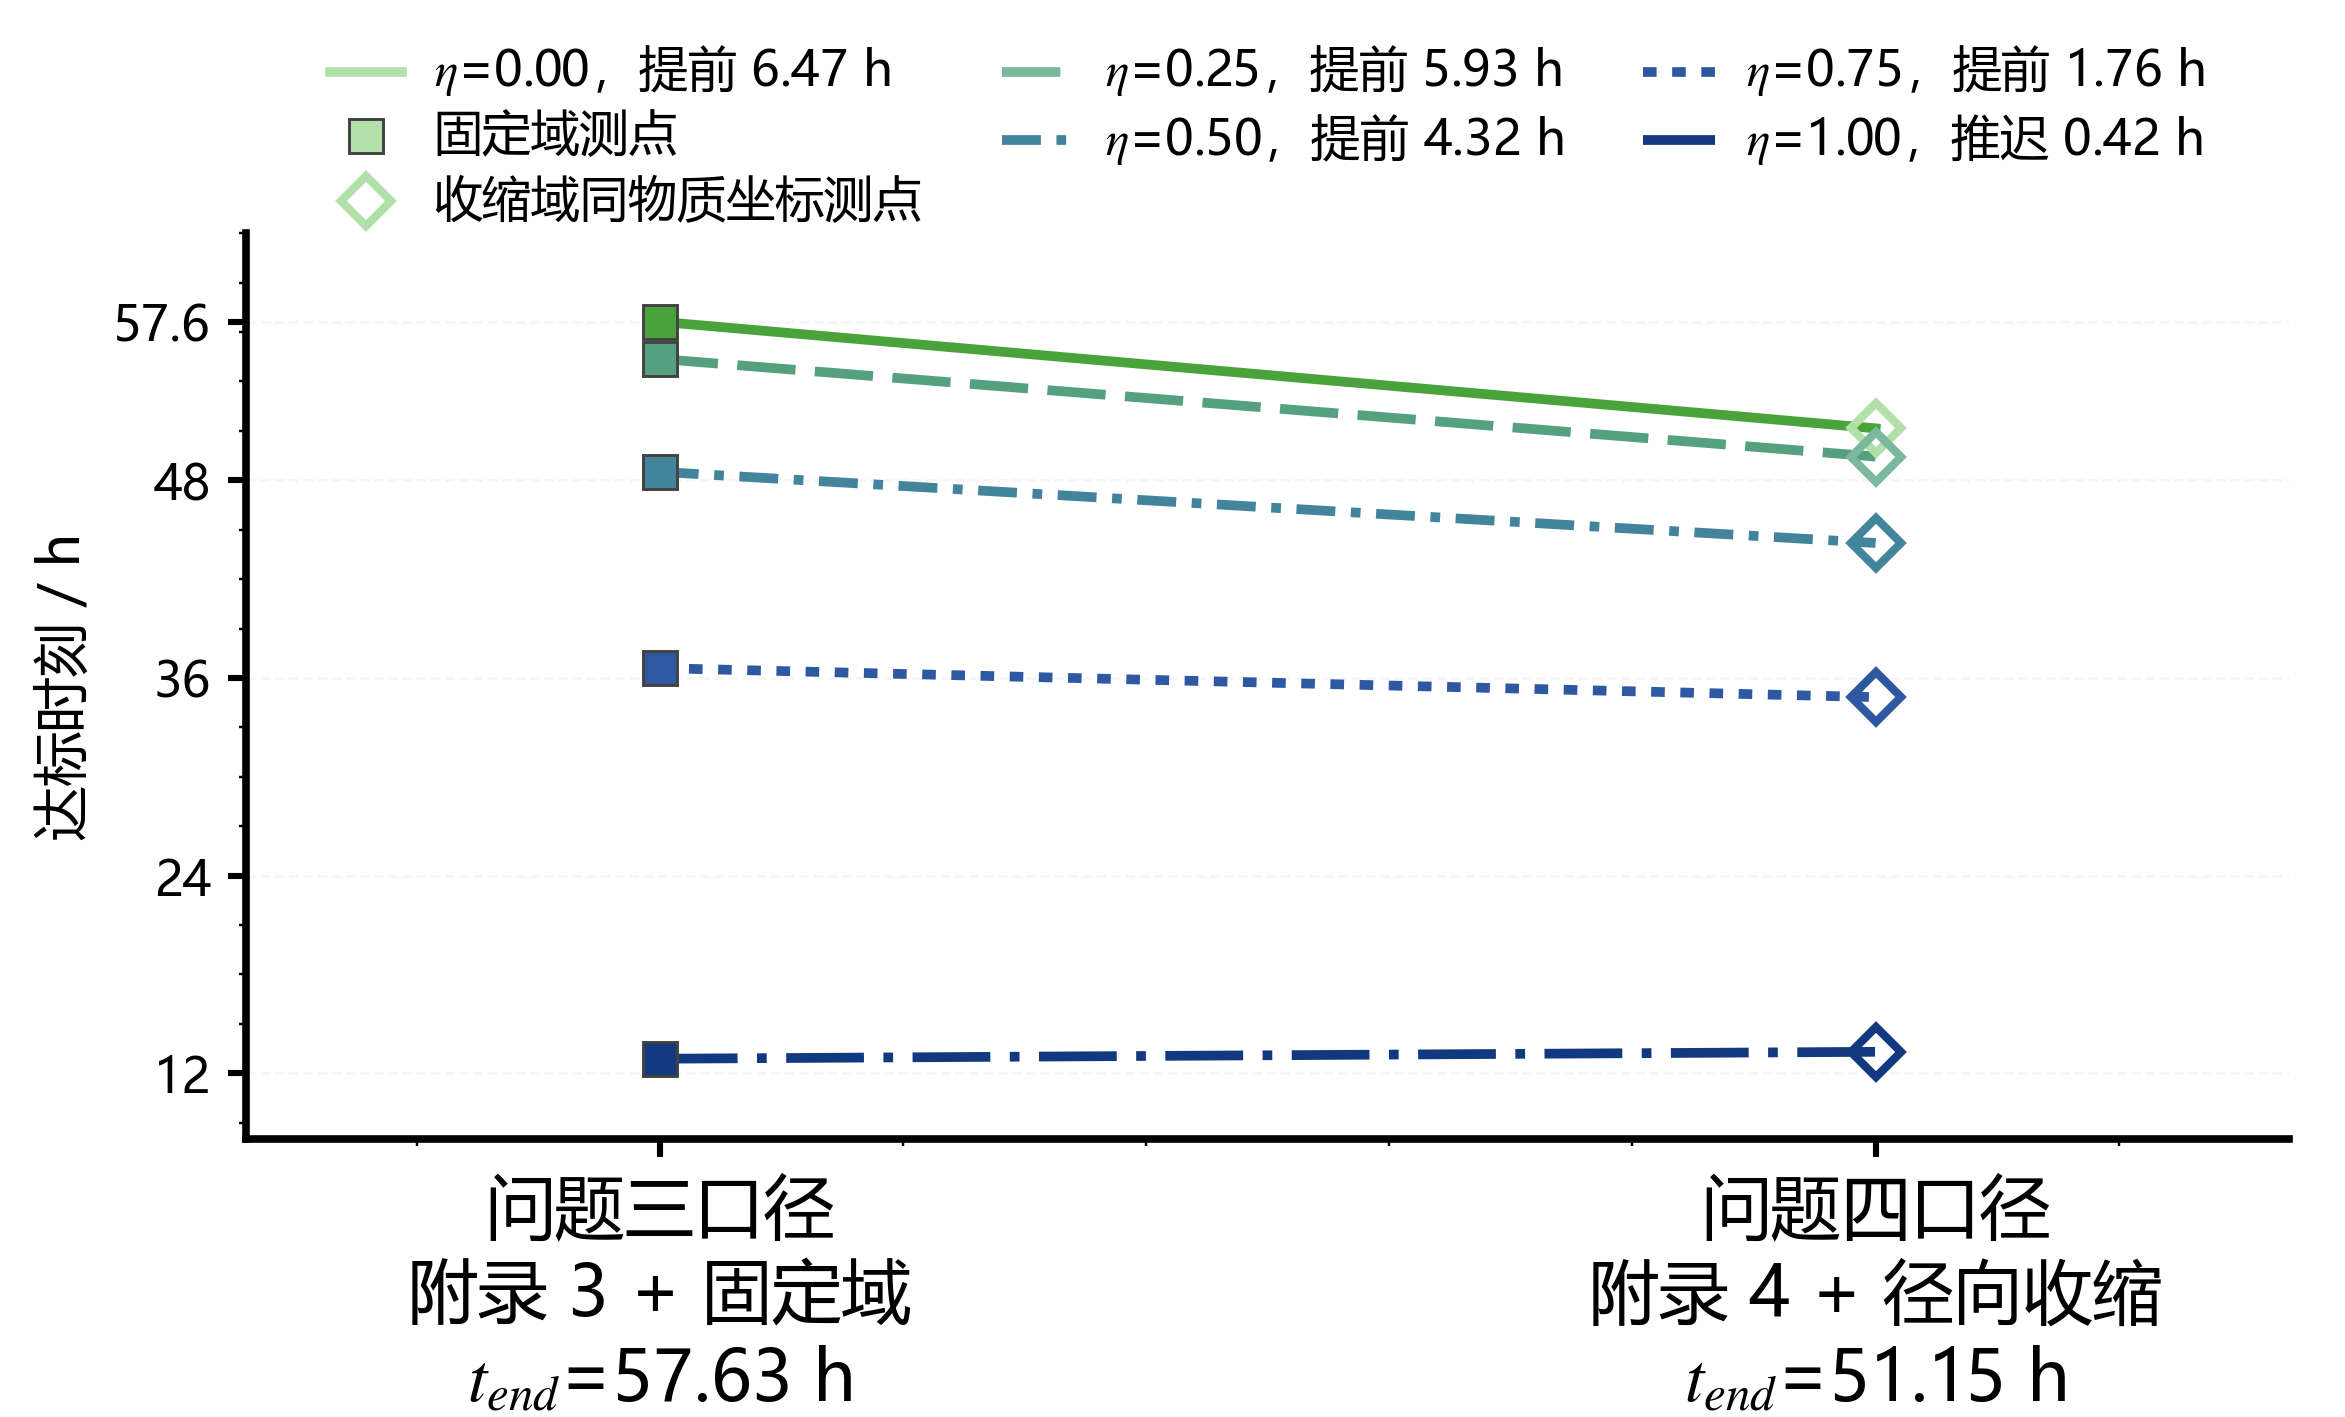
\includegraphics[width=0.92\textwidth]{figures/fig_q4_compare_q3.png}
  \caption[固定域与收缩域达标时刻对照]{固定几何与收缩几何在 5 个物质坐标测点 $\eta=r/R(t)$ 上的达标时刻斜率图。问题三 $R$ 恒为 2\,cm，故 $\eta$ 与固定物理半径一一对应。中心（$\eta$=0）即全域达标时刻，由 57.625\,h 提前至 51.151\,h（缩短 6.474\,h，11.23\%）；表面（$\eta$=1）反而由 12.886\,h 推迟至 13.306\,h。收缩缩短了扩散路径却抬高了表层含水率，两种效应的净结果由中心测点决定。}
  \label{fig:q4_compare_q3}
\end{figure}

\begin{figure}[H]
  \centering
  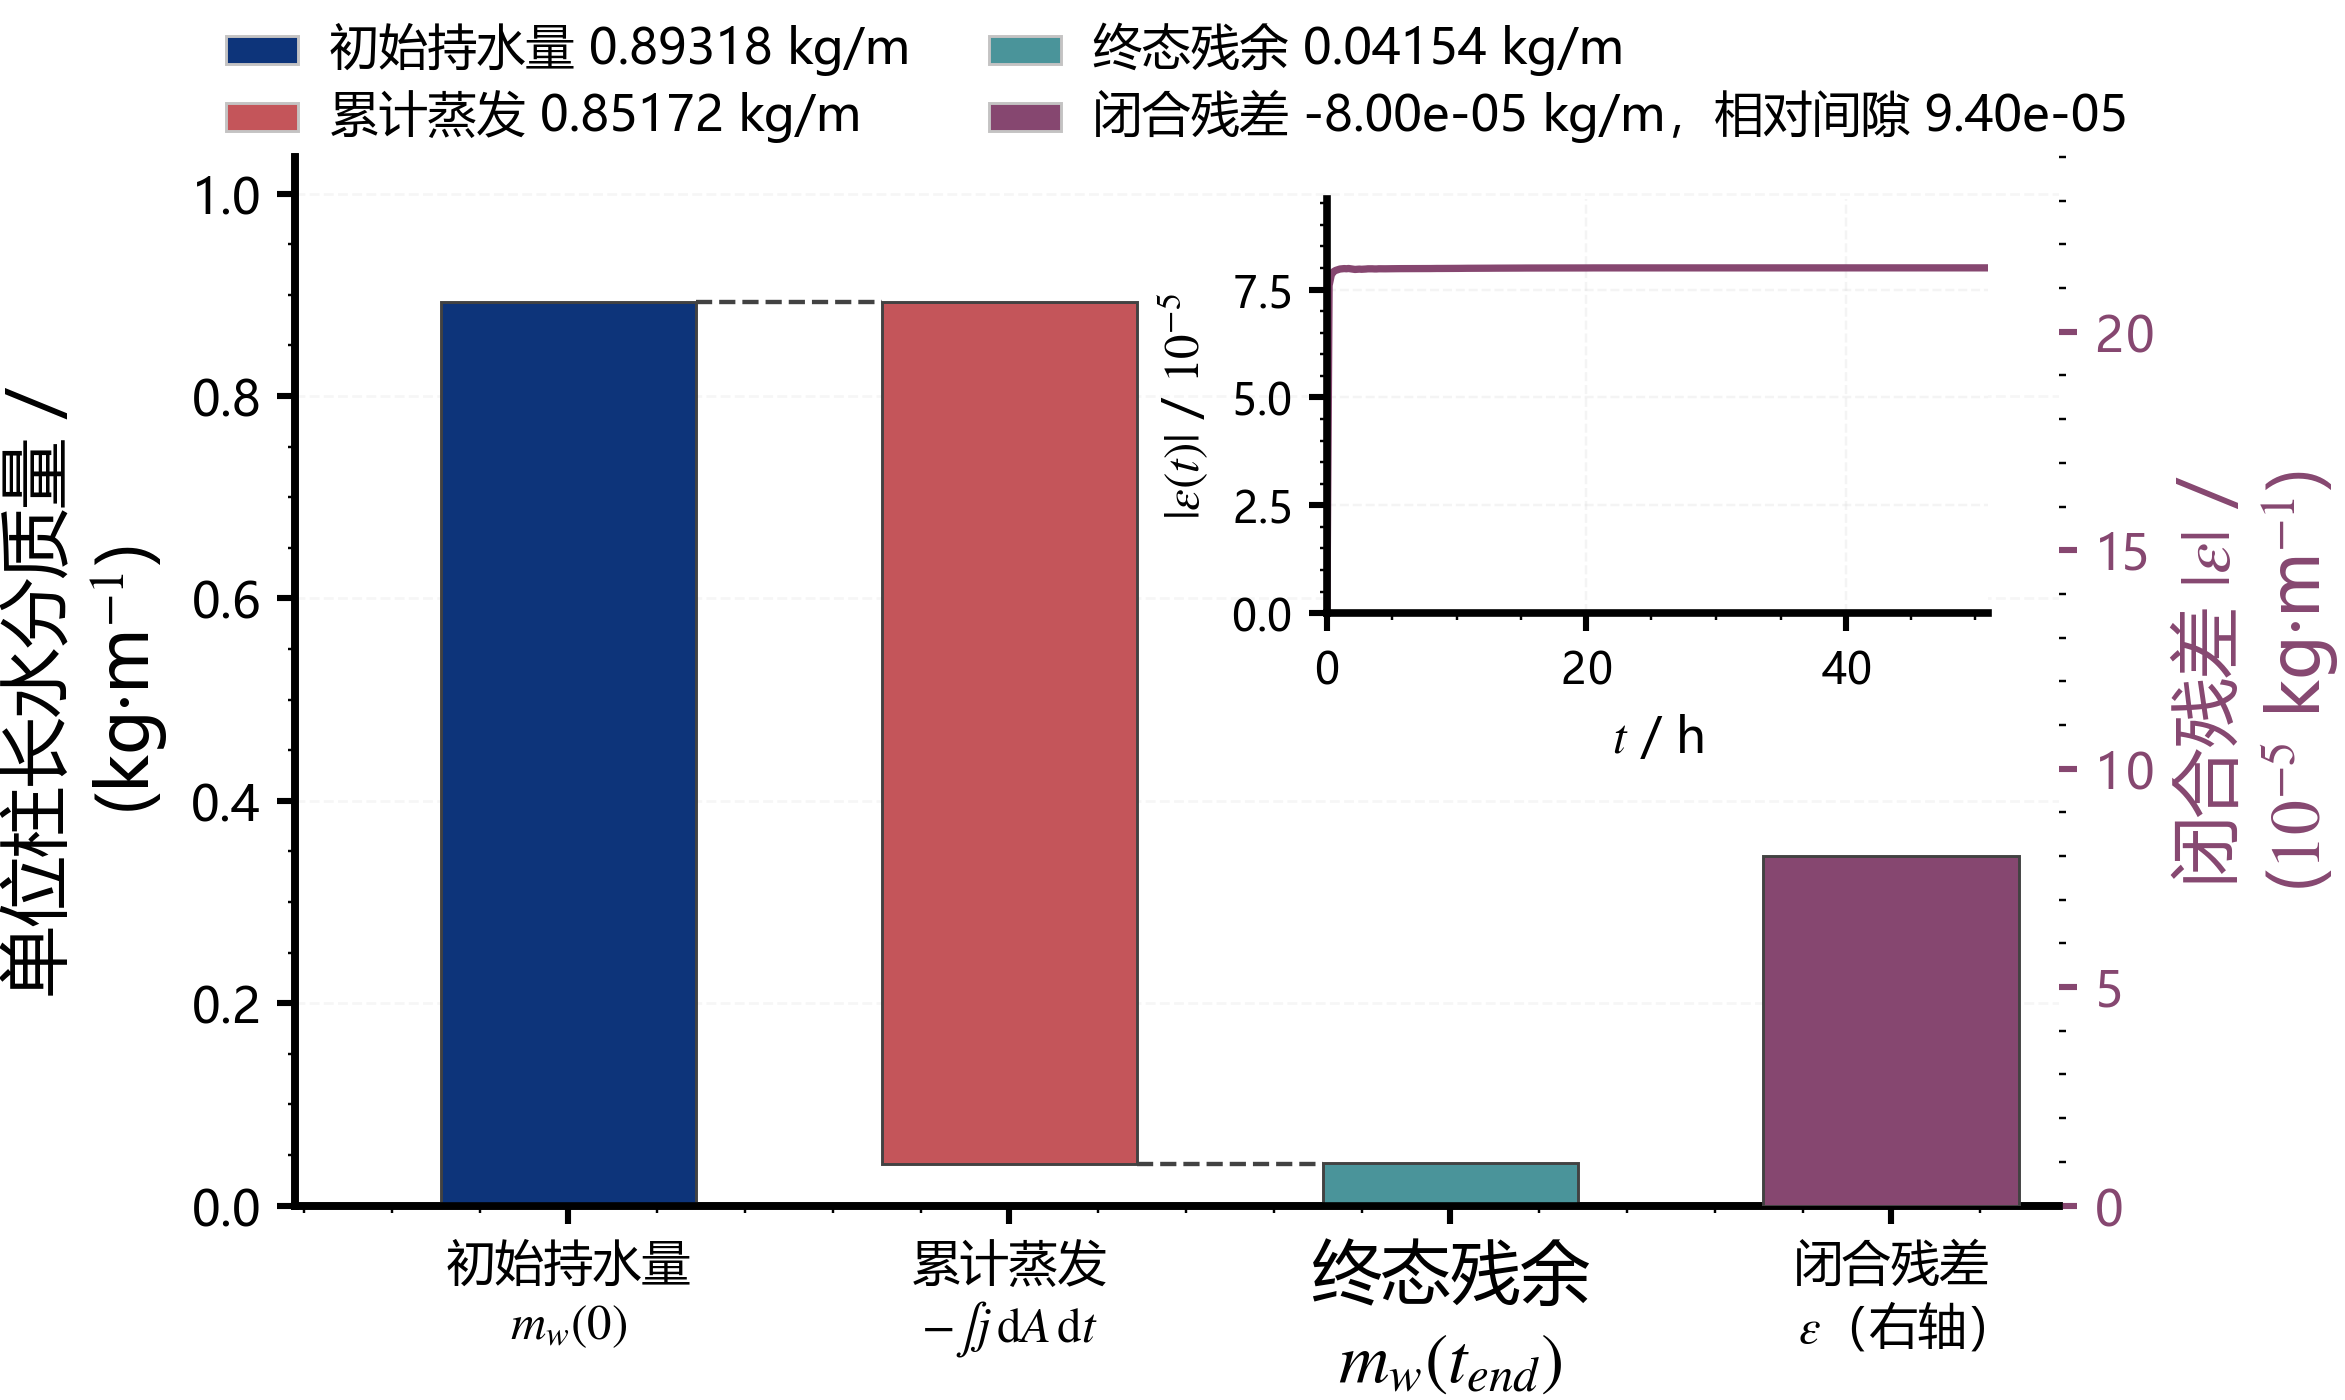
\includegraphics[width=0.92\textwidth]{figures/fig_q4_mass_balance.png}
  \caption[问题四水分质量平衡瀑布图]{问题四水分质量平衡瀑布图：单位柱长初始持水量 0.89318\,kg/m 减去累计蒸发 0.85172\,kg/m 应等于终态残余 0.04154\,kg/m。闭合残差 $8.00\times10^{-5}$\,kg/m 比前三项小四个量级，须用右轴（$10^{-5}$\,kg/m）方能显示；相对间隙 $9.40\times10^{-5}$，低于 $10^{-3}$ 判据。插图给出残差的时间过程，说明闭合性并非只在终点成立。全程脱水率 95.36\%，残差量级与 60\,s 网格上的梯形求积误差相符。}
  \label{fig:q4_mass_balance}
\end{figure}

\begin{figure}[H]
  \centering
  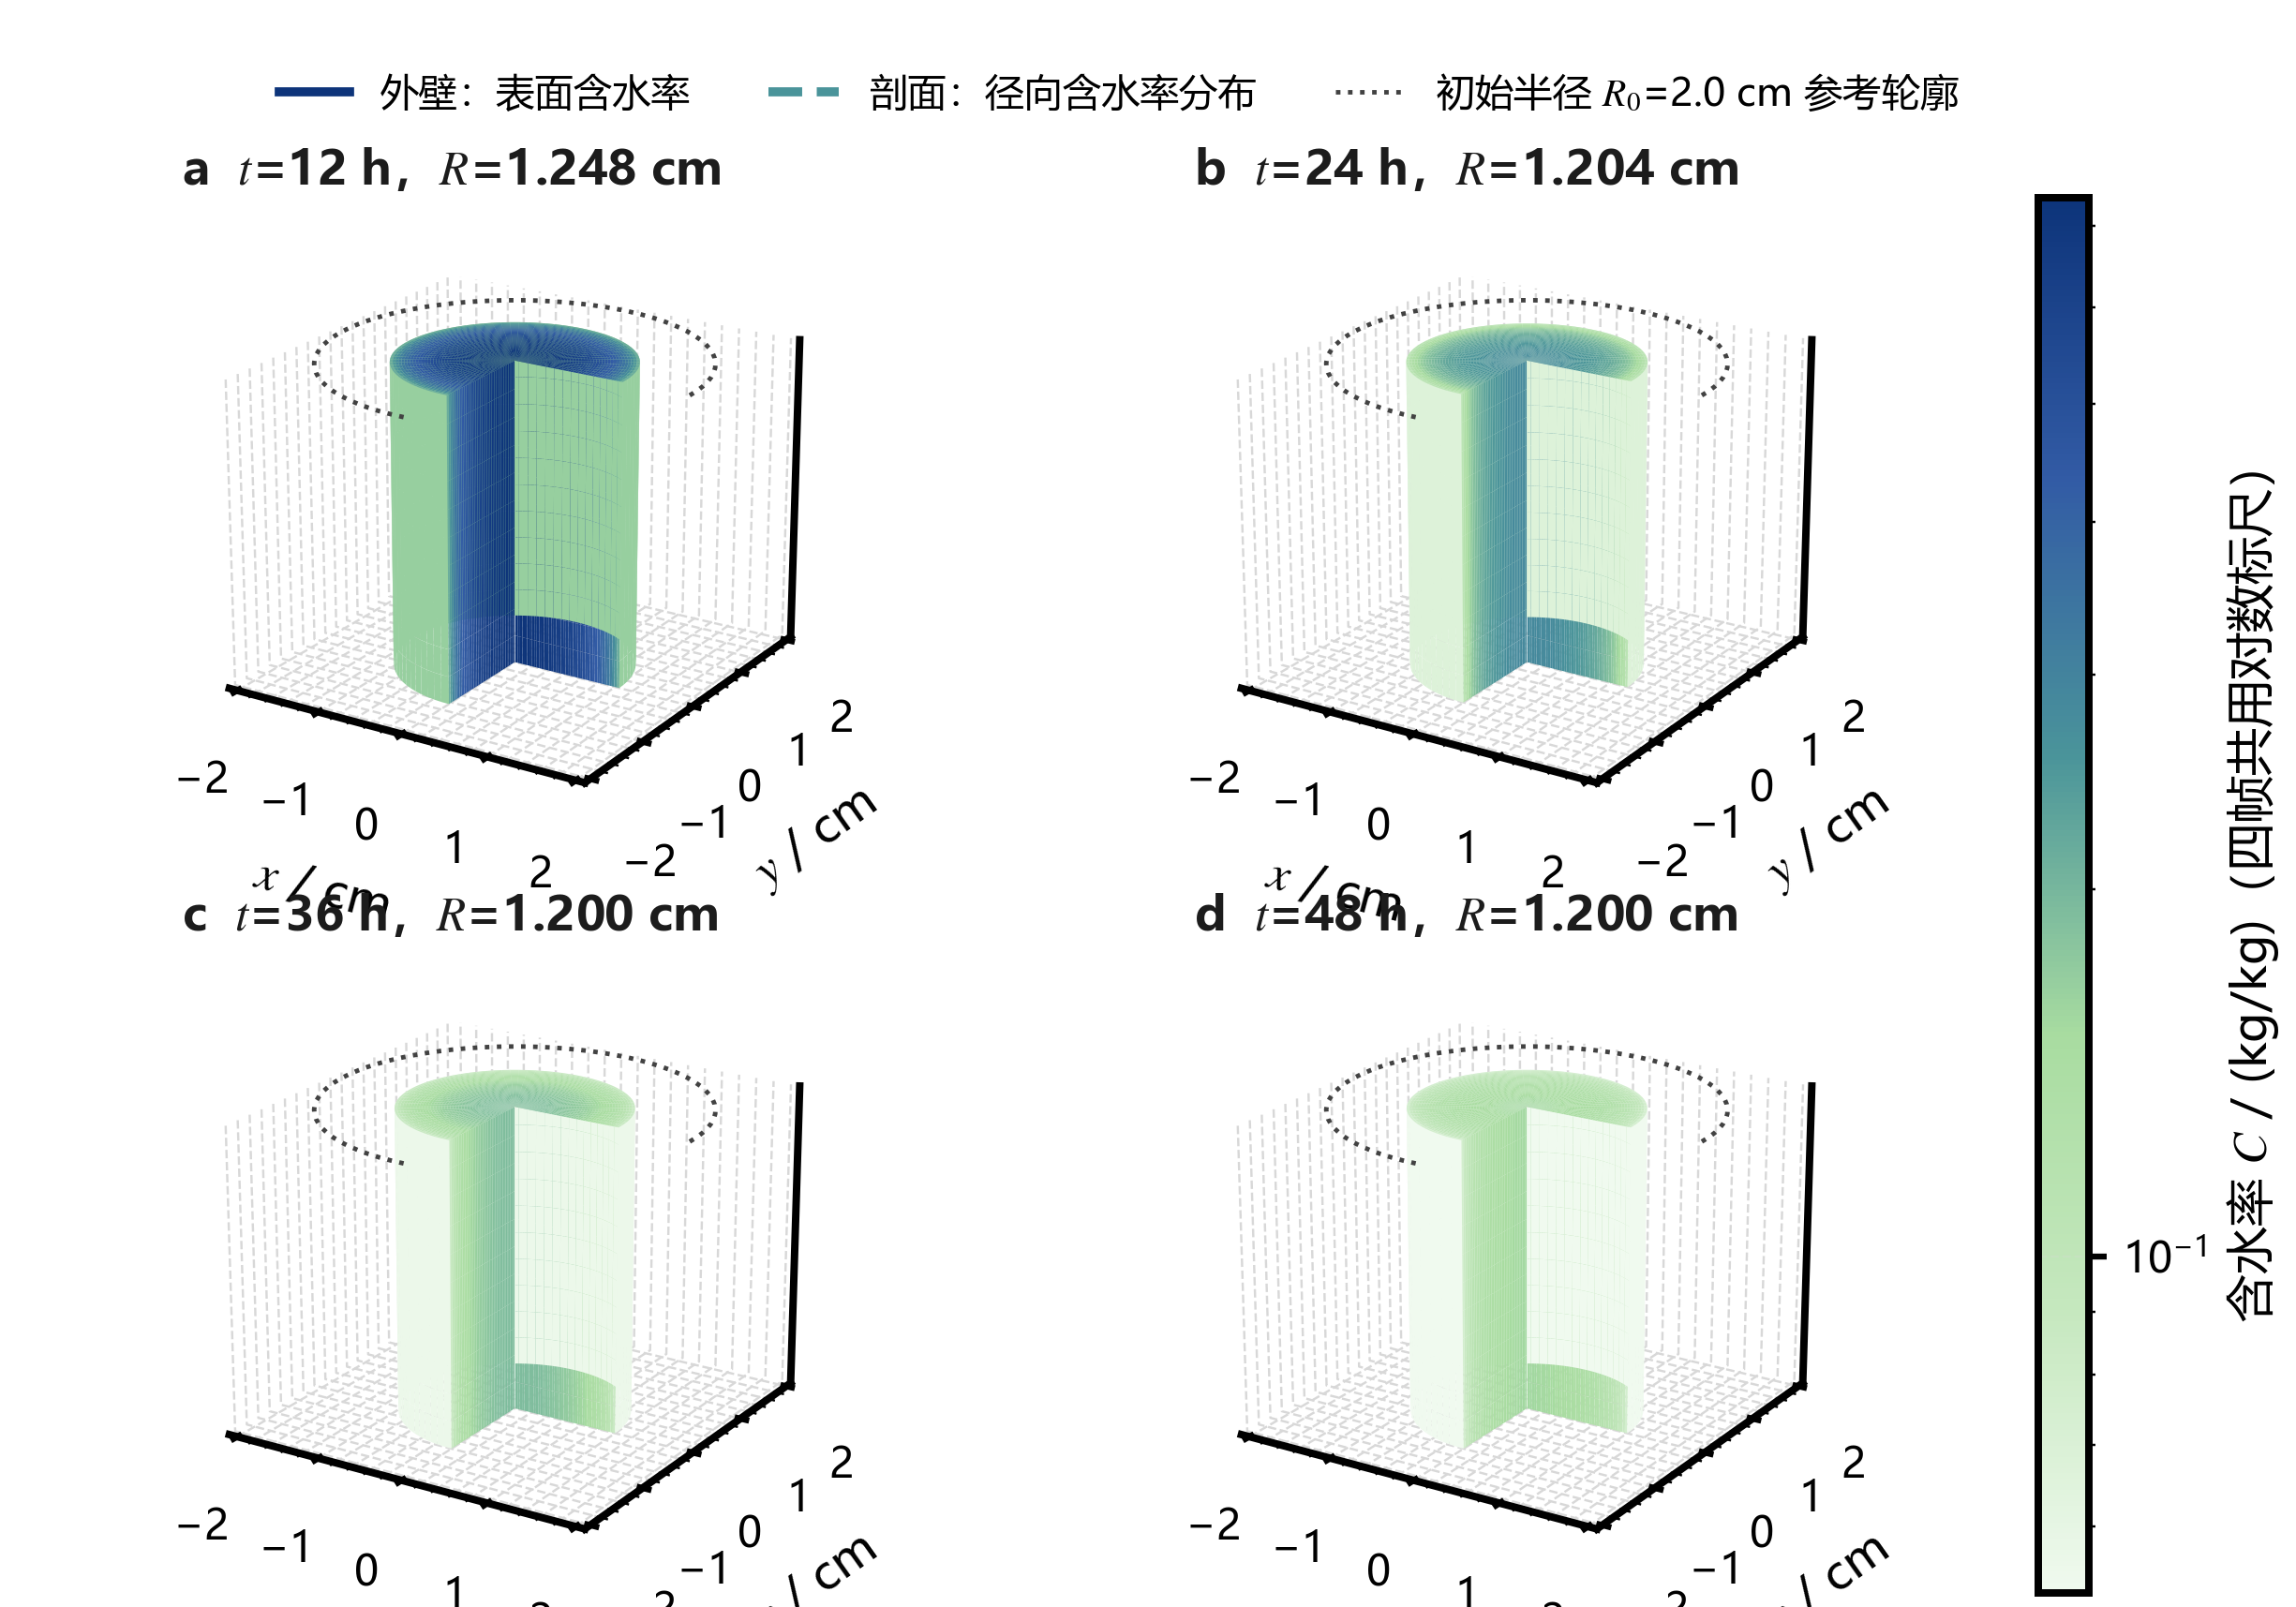
\includegraphics[width=0.96\textwidth]{figures/fig_q4_3d_cylinder.png}
  \caption[问题四圆柱三维剖切渲染四帧]{问题四四帧圆柱三维剖切渲染，剖去 $90^{\circ}$ 楔形以露出内部，外壁与剖面按含水率着色（对数色标），半径按 $R(t)$ 真实值缩放，点线圆为初始外径 $R_0$=2\,cm。四帧 $t$=12/24/36/48\,h 对应 $R$=1.248/1.204/1.200/1.200\,cm。$t_{end}$=51.151\,h 时 $R$=1.2\,cm、绝干密度由 278.7 升至 776.8\,kg/m$^3$，与附录 4 零含水率密度 760\,kg/m$^3$ 相差 2.22\%，故收缩方向判定为径向而非各向同性（后者相差 70.64\%）。}
  \label{fig:q4_3d_cylinder}
\end{figure}
